\documentclass[twoside]{book}

% Packages required by doxygen
\usepackage{fixltx2e}
\usepackage{calc}
\usepackage{doxygen}
\usepackage[export]{adjustbox} % also loads graphicx
\usepackage{graphicx}
\usepackage[utf8]{inputenc}
\usepackage{makeidx}
\usepackage{multicol}
\usepackage{multirow}
\PassOptionsToPackage{warn}{textcomp}
\usepackage{textcomp}
\usepackage[nointegrals]{wasysym}
\usepackage[table]{xcolor}

% Font selection
\usepackage[T1]{fontenc}
\usepackage[scaled=.90]{helvet}
\usepackage{courier}
\usepackage{amssymb}
\usepackage{sectsty}
\renewcommand{\familydefault}{\sfdefault}
\allsectionsfont{%
  \fontseries{bc}\selectfont%
  \color{darkgray}%
}
\renewcommand{\DoxyLabelFont}{%
  \fontseries{bc}\selectfont%
  \color{darkgray}%
}
\newcommand{\+}{\discretionary{\mbox{\scriptsize$\hookleftarrow$}}{}{}}

% Page & text layout
\usepackage{geometry}
\geometry{%
  a4paper,%
  top=2.5cm,%
  bottom=2.5cm,%
  left=2.5cm,%
  right=2.5cm%
}
\tolerance=750
\hfuzz=15pt
\hbadness=750
\setlength{\emergencystretch}{15pt}
\setlength{\parindent}{0cm}
\setlength{\parskip}{0.2cm}
\makeatletter
\renewcommand{\paragraph}{%
  \@startsection{paragraph}{4}{0ex}{-1.0ex}{1.0ex}{%
    \normalfont\normalsize\bfseries\SS@parafont%
  }%
}
\renewcommand{\subparagraph}{%
  \@startsection{subparagraph}{5}{0ex}{-1.0ex}{1.0ex}{%
    \normalfont\normalsize\bfseries\SS@subparafont%
  }%
}
\makeatother

% Headers & footers
\usepackage{fancyhdr}
\pagestyle{fancyplain}
\fancyhead[LE]{\fancyplain{}{\bfseries\thepage}}
\fancyhead[CE]{\fancyplain{}{}}
\fancyhead[RE]{\fancyplain{}{\bfseries\leftmark}}
\fancyhead[LO]{\fancyplain{}{\bfseries\rightmark}}
\fancyhead[CO]{\fancyplain{}{}}
\fancyhead[RO]{\fancyplain{}{\bfseries\thepage}}
\fancyfoot[LE]{\fancyplain{}{}}
\fancyfoot[CE]{\fancyplain{}{}}
\fancyfoot[RE]{\fancyplain{}{\bfseries\scriptsize Generated on Mon Aug 1 2016 18\+:03\+:20 for M\+T\+Gos by Doxygen }}
\fancyfoot[LO]{\fancyplain{}{\bfseries\scriptsize Generated on Mon Aug 1 2016 18\+:03\+:20 for M\+T\+Gos by Doxygen }}
\fancyfoot[CO]{\fancyplain{}{}}
\fancyfoot[RO]{\fancyplain{}{}}
\renewcommand{\footrulewidth}{0.4pt}
\renewcommand{\chaptermark}[1]{%
  \markboth{#1}{}%
}
\renewcommand{\sectionmark}[1]{%
  \markright{\thesection\ #1}%
}

% Indices & bibliography
\usepackage{natbib}
\usepackage[titles]{tocloft}
\setcounter{tocdepth}{3}
\setcounter{secnumdepth}{5}
\makeindex

% Hyperlinks (required, but should be loaded last)
\usepackage{ifpdf}
\ifpdf
  \usepackage[pdftex,pagebackref=true]{hyperref}
\else
  \usepackage[ps2pdf,pagebackref=true]{hyperref}
\fi
\hypersetup{%
  colorlinks=true,%
  linkcolor=blue,%
  citecolor=blue,%
  unicode%
}

% Custom commands
\newcommand{\clearemptydoublepage}{%
  \newpage{\pagestyle{empty}\cleardoublepage}%
}


%===== C O N T E N T S =====

\begin{document}

% Titlepage & ToC
\hypersetup{pageanchor=false,
             bookmarks=true,
             bookmarksnumbered=true,
             pdfencoding=unicode
            }
\pagenumbering{roman}
\begin{titlepage}
\vspace*{7cm}
\begin{center}%
{\Large M\+T\+Gos \\[1ex]\large 0.\+0.\+0 }\\
\vspace*{1cm}
{\large Generated by Doxygen 1.8.10}\\
\vspace*{0.5cm}
{\small Mon Aug 1 2016 18:03:20}\\
\end{center}
\end{titlepage}
\clearemptydoublepage
\tableofcontents
\clearemptydoublepage
\pagenumbering{arabic}
\hypersetup{pageanchor=true}

%--- Begin generated contents ---
\chapter{Namespace Index}
\section{Namespace List}
Here is a list of all namespaces with brief descriptions\+:\begin{DoxyCompactList}
\item\contentsline{section}{\hyperlink{namespace_m_t_gos}{M\+T\+Gos} }{\pageref{namespace_m_t_gos}}{}
\item\contentsline{section}{\hyperlink{namespace_m_t_gos_1_1_base}{M\+T\+Gos\+::\+Base} }{\pageref{namespace_m_t_gos_1_1_base}}{}
\end{DoxyCompactList}

\chapter{Class Index}
\section{Class List}
Here are the classes, structs, unions and interfaces with brief descriptions\+:\begin{DoxyCompactList}
\item\contentsline{section}{\hyperlink{struct_f_i_r_m__header}{F\+I\+R\+M\+\_\+header} \\*Contains the first sector of every F\+I\+R\+M file }{\pageref{struct_f_i_r_m__header}}{}
\item\contentsline{section}{\hyperlink{struct_f_i_r_m__sect}{F\+I\+R\+M\+\_\+sect} \\*Contains one section of the F\+I\+R\+M format }{\pageref{struct_f_i_r_m__sect}}{}
\item\contentsline{section}{\hyperlink{struct_m_o_d_e___i_n_f_o}{M\+O\+D\+E\+\_\+\+I\+N\+F\+O} }{\pageref{struct_m_o_d_e___i_n_f_o}}{}
\item\contentsline{section}{\hyperlink{structmultiboot__aout__symbol__table}{multiboot\+\_\+aout\+\_\+symbol\+\_\+table} }{\pageref{structmultiboot__aout__symbol__table}}{}
\item\contentsline{section}{\hyperlink{structmultiboot__apm__info}{multiboot\+\_\+apm\+\_\+info} }{\pageref{structmultiboot__apm__info}}{}
\item\contentsline{section}{\hyperlink{structmultiboot__color}{multiboot\+\_\+color} }{\pageref{structmultiboot__color}}{}
\item\contentsline{section}{\hyperlink{structmultiboot__elf__section__header__table}{multiboot\+\_\+elf\+\_\+section\+\_\+header\+\_\+table} }{\pageref{structmultiboot__elf__section__header__table}}{}
\item\contentsline{section}{\hyperlink{structmultiboot__header}{multiboot\+\_\+header} }{\pageref{structmultiboot__header}}{}
\item\contentsline{section}{\hyperlink{structmultiboot__info}{multiboot\+\_\+info} }{\pageref{structmultiboot__info}}{}
\item\contentsline{section}{\hyperlink{structmultiboot__mmap__entry}{multiboot\+\_\+mmap\+\_\+entry} }{\pageref{structmultiboot__mmap__entry}}{}
\item\contentsline{section}{\hyperlink{structmultiboot__mod__list}{multiboot\+\_\+mod\+\_\+list} }{\pageref{structmultiboot__mod__list}}{}
\item\contentsline{section}{\hyperlink{class_m_t_gos_1_1_base_1_1_output}{M\+T\+Gos\+::\+Base\+::\+Output} \\*\hyperlink{namespace_m_t_gos_1_1_base}{Base} class for output classes }{\pageref{class_m_t_gos_1_1_base_1_1_output}}{}
\end{DoxyCompactList}

\chapter{File Index}
\section{File List}
Here is a list of all files with brief descriptions\+:\begin{DoxyCompactList}
\item\contentsline{section}{boot/x86/\hyperlink{init_8c}{init.\+c} }{\pageref{init_8c}}{}
\item\contentsline{section}{boot/x86/\hyperlink{multiboot_8h}{multiboot.\+h} }{\pageref{multiboot_8h}}{}
\item\contentsline{section}{c\+\_\+include/\hyperlink{stdint_8h}{stdint.\+h} }{\pageref{stdint_8h}}{}
\item\contentsline{section}{include/base/\hyperlink{output_8hpp}{output.\+hpp} }{\pageref{output_8hpp}}{}
\item\contentsline{section}{kernel/\hyperlink{init_8cpp}{init.\+cpp} }{\pageref{init_8cpp}}{}
\end{DoxyCompactList}

\chapter{Namespace Documentation}
\hypertarget{namespace_m_t_gos}{}\section{M\+T\+Gos Namespace Reference}
\label{namespace_m_t_gos}\index{M\+T\+Gos@{M\+T\+Gos}}
\subsection*{Namespaces}
\begin{DoxyCompactItemize}
\item 
 \hyperlink{namespace_m_t_gos_1_1_base}{Base}
\end{DoxyCompactItemize}

\hypertarget{namespace_m_t_gos_1_1_base}{}\section{M\+T\+Gos\+:\+:Base Namespace Reference}
\label{namespace_m_t_gos_1_1_base}\index{M\+T\+Gos\+::\+Base@{M\+T\+Gos\+::\+Base}}
\subsection*{Classes}
\begin{DoxyCompactItemize}
\item 
class \hyperlink{class_m_t_gos_1_1_base_1_1_output}{Output}
\begin{DoxyCompactList}\small\item\em \hyperlink{namespace_m_t_gos_1_1_base}{Base} class for output classes. \end{DoxyCompactList}\end{DoxyCompactItemize}
\subsection*{Enumerations}
\begin{DoxyCompactItemize}
\item 
enum \hyperlink{namespace_m_t_gos_1_1_base_a985066b1d1e61799ead33462c57496a1}{Base} \+: int \{ \\*
\hyperlink{namespace_m_t_gos_1_1_base_a985066b1d1e61799ead33462c57496a1a98ad0e8750ae10ad556ed7a62affb452}{Base\+::\+B\+I\+N\+A\+R\+Y} =2, 
\hyperlink{namespace_m_t_gos_1_1_base_a985066b1d1e61799ead33462c57496a1a8343ca237665c0d9e59cb1b668462f70}{Base\+::\+T\+E\+R\+N\+A\+R\+Y}, 
\hyperlink{namespace_m_t_gos_1_1_base_a985066b1d1e61799ead33462c57496a1a318b856f74594843844042bf9ab09ec1}{Base\+::\+B\+A\+S\+E4}, 
\hyperlink{namespace_m_t_gos_1_1_base_a985066b1d1e61799ead33462c57496a1a55197e0b604bcd695580d3195dee8bda}{Base\+::\+B\+A\+S\+E5}, 
\\*
\hyperlink{namespace_m_t_gos_1_1_base_a985066b1d1e61799ead33462c57496a1ab32f9567b422b1314a04fb70e46eefc3}{Base\+::\+B\+A\+S\+E6}, 
\hyperlink{namespace_m_t_gos_1_1_base_a985066b1d1e61799ead33462c57496a1aa6e517afa675ea5e7475f2ec0b5d1ea5}{Base\+::\+B\+A\+S\+E7}, 
\hyperlink{namespace_m_t_gos_1_1_base_a985066b1d1e61799ead33462c57496a1a62bfcf2abd9e92ff5e7cc7f6aa552d14}{Base\+::\+O\+C\+T\+A\+L}, 
\hyperlink{namespace_m_t_gos_1_1_base_a985066b1d1e61799ead33462c57496a1ae010292b0e1e622ba25a7e74a057703d}{Base\+::\+B\+A\+S\+E9}, 
\\*
\hyperlink{namespace_m_t_gos_1_1_base_a985066b1d1e61799ead33462c57496a1a13d992d671957e9a2b3e936ca0cf14a4}{Base\+::\+D\+E\+C\+I\+M\+A\+L}, 
\hyperlink{namespace_m_t_gos_1_1_base_a985066b1d1e61799ead33462c57496a1af2a8c7e523d8164420af80aa37725e61}{Base\+::\+B\+A\+S\+E11}, 
\hyperlink{namespace_m_t_gos_1_1_base_a985066b1d1e61799ead33462c57496a1a019b38414fbc79cd8a902243389392f9}{Base\+::\+B\+A\+S\+E12}, 
\hyperlink{namespace_m_t_gos_1_1_base_a985066b1d1e61799ead33462c57496a1a3b11e53a4cc9342c948976ff40488cbf}{Base\+::\+B\+A\+S\+E13}, 
\\*
\hyperlink{namespace_m_t_gos_1_1_base_a985066b1d1e61799ead33462c57496a1a8ffa2305b0c97880be705d0b1144e26a}{Base\+::\+B\+A\+S\+E14}, 
\hyperlink{namespace_m_t_gos_1_1_base_a985066b1d1e61799ead33462c57496a1ae0e888f5dc8a328cc1281a61b5b7352d}{Base\+::\+B\+A\+S\+E15}, 
\hyperlink{namespace_m_t_gos_1_1_base_a985066b1d1e61799ead33462c57496a1a99f7a3f3b35d3a43505b79198b698b84}{Base\+::\+H\+E\+X\+A\+D\+E\+C\+I\+M\+A\+L}
 \}\begin{DoxyCompactList}\small\item\em Contains the useable bases in the number-\/printing routine. \end{DoxyCompactList}
\end{DoxyCompactItemize}


\subsection{Enumeration Type Documentation}
\hypertarget{namespace_m_t_gos_1_1_base_a985066b1d1e61799ead33462c57496a1}{}\index{M\+T\+Gos\+::\+Base@{M\+T\+Gos\+::\+Base}!Base@{Base}}
\index{Base@{Base}!M\+T\+Gos\+::\+Base@{M\+T\+Gos\+::\+Base}}
\subsubsection[{Base}]{\setlength{\rightskip}{0pt plus 5cm}enum {\bf M\+T\+Gos\+::\+Base\+::\+Base} \+: int\hspace{0.3cm}{\ttfamily [strong]}}\label{namespace_m_t_gos_1_1_base_a985066b1d1e61799ead33462c57496a1}


Contains the useable bases in the number-\/printing routine. 

\begin{Desc}
\item[Enumerator]\par
\begin{description}
\index{B\+I\+N\+A\+R\+Y@{B\+I\+N\+A\+R\+Y}!M\+T\+Gos\+::\+Base@{M\+T\+Gos\+::\+Base}}\index{M\+T\+Gos\+::\+Base@{M\+T\+Gos\+::\+Base}!B\+I\+N\+A\+R\+Y@{B\+I\+N\+A\+R\+Y}}\item[{\em 
\hypertarget{namespace_m_t_gos_1_1_base_a985066b1d1e61799ead33462c57496a1a98ad0e8750ae10ad556ed7a62affb452}{}B\+I\+N\+A\+R\+Y\label{namespace_m_t_gos_1_1_base_a985066b1d1e61799ead33462c57496a1a98ad0e8750ae10ad556ed7a62affb452}
}]\index{T\+E\+R\+N\+A\+R\+Y@{T\+E\+R\+N\+A\+R\+Y}!M\+T\+Gos\+::\+Base@{M\+T\+Gos\+::\+Base}}\index{M\+T\+Gos\+::\+Base@{M\+T\+Gos\+::\+Base}!T\+E\+R\+N\+A\+R\+Y@{T\+E\+R\+N\+A\+R\+Y}}\item[{\em 
\hypertarget{namespace_m_t_gos_1_1_base_a985066b1d1e61799ead33462c57496a1a8343ca237665c0d9e59cb1b668462f70}{}T\+E\+R\+N\+A\+R\+Y\label{namespace_m_t_gos_1_1_base_a985066b1d1e61799ead33462c57496a1a8343ca237665c0d9e59cb1b668462f70}
}]\index{B\+A\+S\+E4@{B\+A\+S\+E4}!M\+T\+Gos\+::\+Base@{M\+T\+Gos\+::\+Base}}\index{M\+T\+Gos\+::\+Base@{M\+T\+Gos\+::\+Base}!B\+A\+S\+E4@{B\+A\+S\+E4}}\item[{\em 
\hypertarget{namespace_m_t_gos_1_1_base_a985066b1d1e61799ead33462c57496a1a318b856f74594843844042bf9ab09ec1}{}B\+A\+S\+E4\label{namespace_m_t_gos_1_1_base_a985066b1d1e61799ead33462c57496a1a318b856f74594843844042bf9ab09ec1}
}]\index{B\+A\+S\+E5@{B\+A\+S\+E5}!M\+T\+Gos\+::\+Base@{M\+T\+Gos\+::\+Base}}\index{M\+T\+Gos\+::\+Base@{M\+T\+Gos\+::\+Base}!B\+A\+S\+E5@{B\+A\+S\+E5}}\item[{\em 
\hypertarget{namespace_m_t_gos_1_1_base_a985066b1d1e61799ead33462c57496a1a55197e0b604bcd695580d3195dee8bda}{}B\+A\+S\+E5\label{namespace_m_t_gos_1_1_base_a985066b1d1e61799ead33462c57496a1a55197e0b604bcd695580d3195dee8bda}
}]\index{B\+A\+S\+E6@{B\+A\+S\+E6}!M\+T\+Gos\+::\+Base@{M\+T\+Gos\+::\+Base}}\index{M\+T\+Gos\+::\+Base@{M\+T\+Gos\+::\+Base}!B\+A\+S\+E6@{B\+A\+S\+E6}}\item[{\em 
\hypertarget{namespace_m_t_gos_1_1_base_a985066b1d1e61799ead33462c57496a1ab32f9567b422b1314a04fb70e46eefc3}{}B\+A\+S\+E6\label{namespace_m_t_gos_1_1_base_a985066b1d1e61799ead33462c57496a1ab32f9567b422b1314a04fb70e46eefc3}
}]\index{B\+A\+S\+E7@{B\+A\+S\+E7}!M\+T\+Gos\+::\+Base@{M\+T\+Gos\+::\+Base}}\index{M\+T\+Gos\+::\+Base@{M\+T\+Gos\+::\+Base}!B\+A\+S\+E7@{B\+A\+S\+E7}}\item[{\em 
\hypertarget{namespace_m_t_gos_1_1_base_a985066b1d1e61799ead33462c57496a1aa6e517afa675ea5e7475f2ec0b5d1ea5}{}B\+A\+S\+E7\label{namespace_m_t_gos_1_1_base_a985066b1d1e61799ead33462c57496a1aa6e517afa675ea5e7475f2ec0b5d1ea5}
}]\index{O\+C\+T\+A\+L@{O\+C\+T\+A\+L}!M\+T\+Gos\+::\+Base@{M\+T\+Gos\+::\+Base}}\index{M\+T\+Gos\+::\+Base@{M\+T\+Gos\+::\+Base}!O\+C\+T\+A\+L@{O\+C\+T\+A\+L}}\item[{\em 
\hypertarget{namespace_m_t_gos_1_1_base_a985066b1d1e61799ead33462c57496a1a62bfcf2abd9e92ff5e7cc7f6aa552d14}{}O\+C\+T\+A\+L\label{namespace_m_t_gos_1_1_base_a985066b1d1e61799ead33462c57496a1a62bfcf2abd9e92ff5e7cc7f6aa552d14}
}]\index{B\+A\+S\+E9@{B\+A\+S\+E9}!M\+T\+Gos\+::\+Base@{M\+T\+Gos\+::\+Base}}\index{M\+T\+Gos\+::\+Base@{M\+T\+Gos\+::\+Base}!B\+A\+S\+E9@{B\+A\+S\+E9}}\item[{\em 
\hypertarget{namespace_m_t_gos_1_1_base_a985066b1d1e61799ead33462c57496a1ae010292b0e1e622ba25a7e74a057703d}{}B\+A\+S\+E9\label{namespace_m_t_gos_1_1_base_a985066b1d1e61799ead33462c57496a1ae010292b0e1e622ba25a7e74a057703d}
}]\index{D\+E\+C\+I\+M\+A\+L@{D\+E\+C\+I\+M\+A\+L}!M\+T\+Gos\+::\+Base@{M\+T\+Gos\+::\+Base}}\index{M\+T\+Gos\+::\+Base@{M\+T\+Gos\+::\+Base}!D\+E\+C\+I\+M\+A\+L@{D\+E\+C\+I\+M\+A\+L}}\item[{\em 
\hypertarget{namespace_m_t_gos_1_1_base_a985066b1d1e61799ead33462c57496a1a13d992d671957e9a2b3e936ca0cf14a4}{}D\+E\+C\+I\+M\+A\+L\label{namespace_m_t_gos_1_1_base_a985066b1d1e61799ead33462c57496a1a13d992d671957e9a2b3e936ca0cf14a4}
}]\index{B\+A\+S\+E11@{B\+A\+S\+E11}!M\+T\+Gos\+::\+Base@{M\+T\+Gos\+::\+Base}}\index{M\+T\+Gos\+::\+Base@{M\+T\+Gos\+::\+Base}!B\+A\+S\+E11@{B\+A\+S\+E11}}\item[{\em 
\hypertarget{namespace_m_t_gos_1_1_base_a985066b1d1e61799ead33462c57496a1af2a8c7e523d8164420af80aa37725e61}{}B\+A\+S\+E11\label{namespace_m_t_gos_1_1_base_a985066b1d1e61799ead33462c57496a1af2a8c7e523d8164420af80aa37725e61}
}]\index{B\+A\+S\+E12@{B\+A\+S\+E12}!M\+T\+Gos\+::\+Base@{M\+T\+Gos\+::\+Base}}\index{M\+T\+Gos\+::\+Base@{M\+T\+Gos\+::\+Base}!B\+A\+S\+E12@{B\+A\+S\+E12}}\item[{\em 
\hypertarget{namespace_m_t_gos_1_1_base_a985066b1d1e61799ead33462c57496a1a019b38414fbc79cd8a902243389392f9}{}B\+A\+S\+E12\label{namespace_m_t_gos_1_1_base_a985066b1d1e61799ead33462c57496a1a019b38414fbc79cd8a902243389392f9}
}]\index{B\+A\+S\+E13@{B\+A\+S\+E13}!M\+T\+Gos\+::\+Base@{M\+T\+Gos\+::\+Base}}\index{M\+T\+Gos\+::\+Base@{M\+T\+Gos\+::\+Base}!B\+A\+S\+E13@{B\+A\+S\+E13}}\item[{\em 
\hypertarget{namespace_m_t_gos_1_1_base_a985066b1d1e61799ead33462c57496a1a3b11e53a4cc9342c948976ff40488cbf}{}B\+A\+S\+E13\label{namespace_m_t_gos_1_1_base_a985066b1d1e61799ead33462c57496a1a3b11e53a4cc9342c948976ff40488cbf}
}]\index{B\+A\+S\+E14@{B\+A\+S\+E14}!M\+T\+Gos\+::\+Base@{M\+T\+Gos\+::\+Base}}\index{M\+T\+Gos\+::\+Base@{M\+T\+Gos\+::\+Base}!B\+A\+S\+E14@{B\+A\+S\+E14}}\item[{\em 
\hypertarget{namespace_m_t_gos_1_1_base_a985066b1d1e61799ead33462c57496a1a8ffa2305b0c97880be705d0b1144e26a}{}B\+A\+S\+E14\label{namespace_m_t_gos_1_1_base_a985066b1d1e61799ead33462c57496a1a8ffa2305b0c97880be705d0b1144e26a}
}]\index{B\+A\+S\+E15@{B\+A\+S\+E15}!M\+T\+Gos\+::\+Base@{M\+T\+Gos\+::\+Base}}\index{M\+T\+Gos\+::\+Base@{M\+T\+Gos\+::\+Base}!B\+A\+S\+E15@{B\+A\+S\+E15}}\item[{\em 
\hypertarget{namespace_m_t_gos_1_1_base_a985066b1d1e61799ead33462c57496a1ae0e888f5dc8a328cc1281a61b5b7352d}{}B\+A\+S\+E15\label{namespace_m_t_gos_1_1_base_a985066b1d1e61799ead33462c57496a1ae0e888f5dc8a328cc1281a61b5b7352d}
}]\index{H\+E\+X\+A\+D\+E\+C\+I\+M\+A\+L@{H\+E\+X\+A\+D\+E\+C\+I\+M\+A\+L}!M\+T\+Gos\+::\+Base@{M\+T\+Gos\+::\+Base}}\index{M\+T\+Gos\+::\+Base@{M\+T\+Gos\+::\+Base}!H\+E\+X\+A\+D\+E\+C\+I\+M\+A\+L@{H\+E\+X\+A\+D\+E\+C\+I\+M\+A\+L}}\item[{\em 
\hypertarget{namespace_m_t_gos_1_1_base_a985066b1d1e61799ead33462c57496a1a99f7a3f3b35d3a43505b79198b698b84}{}H\+E\+X\+A\+D\+E\+C\+I\+M\+A\+L\label{namespace_m_t_gos_1_1_base_a985066b1d1e61799ead33462c57496a1a99f7a3f3b35d3a43505b79198b698b84}
}]\end{description}
\end{Desc}

\chapter{Class Documentation}
\hypertarget{struct_f_i_r_m__header}{}\section{F\+I\+R\+M\+\_\+header Struct Reference}
\label{struct_f_i_r_m__header}\index{F\+I\+R\+M\+\_\+header@{F\+I\+R\+M\+\_\+header}}


Contains the first sector of every F\+I\+R\+M file.  




Collaboration diagram for F\+I\+R\+M\+\_\+header\+:\nopagebreak
\begin{figure}[H]
\begin{center}
\leavevmode
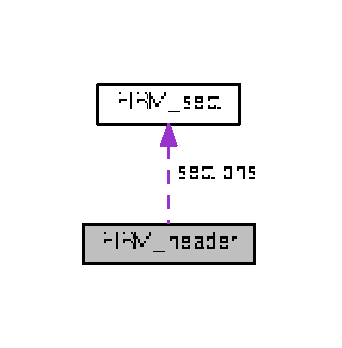
\includegraphics[width=164pt]{struct_f_i_r_m__header__coll__graph}
\end{center}
\end{figure}
\subsection*{Public Attributes}
\begin{DoxyCompactItemize}
\item 
char \hyperlink{struct_f_i_r_m__header_a2d27c5c398bee211d2410fbdbaa5a05e}{magic} \mbox{[}4\mbox{]}
\item 
int \hyperlink{struct_f_i_r_m__header_a3a3ccecb2f6348d0071ce98d102e8a22}{version}
\begin{DoxyCompactList}\small\item\em Magic \char`\"{}\+F\+I\+R\+M\char`\"{} string (not-\/null terminated) \end{DoxyCompactList}\item 
void($\ast$ \hyperlink{struct_f_i_r_m__header_ad1612a664851fdd7f9ca671af2bfc431}{entrypoint} )()
\begin{DoxyCompactList}\small\item\em Version. Currently 1. \end{DoxyCompactList}\item 
unsigned int \hyperlink{struct_f_i_r_m__header_adc471470dba61f85b71e72ee4d84d73e}{reserved} \mbox{[}0x\+D\mbox{]}
\begin{DoxyCompactList}\small\item\em Address where the processor jumps to after loading. \end{DoxyCompactList}\item 
struct \hyperlink{struct_f_i_r_m__sect}{F\+I\+R\+M\+\_\+sect} \hyperlink{struct_f_i_r_m__header_a685b6a1c1a0cfb8fb0f1dfcba06b9741}{sections} \mbox{[}4\mbox{]}
\item 
unsigned char \hyperlink{struct_f_i_r_m__header_a7be52a7b7994c1013d02e2e9e523316b}{R\+S\+A2048} \mbox{[}0x100\mbox{]}
\begin{DoxyCompactList}\small\item\em The four internal sections. \end{DoxyCompactList}\end{DoxyCompactItemize}


\subsection{Detailed Description}
Contains the first sector of every F\+I\+R\+M file. 

\subsection{Member Data Documentation}
\hypertarget{struct_f_i_r_m__header_ad1612a664851fdd7f9ca671af2bfc431}{}\index{F\+I\+R\+M\+\_\+header@{F\+I\+R\+M\+\_\+header}!entrypoint@{entrypoint}}
\index{entrypoint@{entrypoint}!F\+I\+R\+M\+\_\+header@{F\+I\+R\+M\+\_\+header}}
\subsubsection[{entrypoint}]{\setlength{\rightskip}{0pt plus 5cm}void($\ast$ F\+I\+R\+M\+\_\+header\+::entrypoint) ()}\label{struct_f_i_r_m__header_ad1612a664851fdd7f9ca671af2bfc431}


Version. Currently 1. 

\hypertarget{struct_f_i_r_m__header_a2d27c5c398bee211d2410fbdbaa5a05e}{}\index{F\+I\+R\+M\+\_\+header@{F\+I\+R\+M\+\_\+header}!magic@{magic}}
\index{magic@{magic}!F\+I\+R\+M\+\_\+header@{F\+I\+R\+M\+\_\+header}}
\subsubsection[{magic}]{\setlength{\rightskip}{0pt plus 5cm}char F\+I\+R\+M\+\_\+header\+::magic\mbox{[}4\mbox{]}}\label{struct_f_i_r_m__header_a2d27c5c398bee211d2410fbdbaa5a05e}
\hypertarget{struct_f_i_r_m__header_adc471470dba61f85b71e72ee4d84d73e}{}\index{F\+I\+R\+M\+\_\+header@{F\+I\+R\+M\+\_\+header}!reserved@{reserved}}
\index{reserved@{reserved}!F\+I\+R\+M\+\_\+header@{F\+I\+R\+M\+\_\+header}}
\subsubsection[{reserved}]{\setlength{\rightskip}{0pt plus 5cm}unsigned int F\+I\+R\+M\+\_\+header\+::reserved\mbox{[}0x\+D\mbox{]}}\label{struct_f_i_r_m__header_adc471470dba61f85b71e72ee4d84d73e}


Address where the processor jumps to after loading. 

\hypertarget{struct_f_i_r_m__header_a7be52a7b7994c1013d02e2e9e523316b}{}\index{F\+I\+R\+M\+\_\+header@{F\+I\+R\+M\+\_\+header}!R\+S\+A2048@{R\+S\+A2048}}
\index{R\+S\+A2048@{R\+S\+A2048}!F\+I\+R\+M\+\_\+header@{F\+I\+R\+M\+\_\+header}}
\subsubsection[{R\+S\+A2048}]{\setlength{\rightskip}{0pt plus 5cm}unsigned char F\+I\+R\+M\+\_\+header\+::\+R\+S\+A2048\mbox{[}0x100\mbox{]}}\label{struct_f_i_r_m__header_a7be52a7b7994c1013d02e2e9e523316b}


The four internal sections. 

\hypertarget{struct_f_i_r_m__header_a685b6a1c1a0cfb8fb0f1dfcba06b9741}{}\index{F\+I\+R\+M\+\_\+header@{F\+I\+R\+M\+\_\+header}!sections@{sections}}
\index{sections@{sections}!F\+I\+R\+M\+\_\+header@{F\+I\+R\+M\+\_\+header}}
\subsubsection[{sections}]{\setlength{\rightskip}{0pt plus 5cm}struct {\bf F\+I\+R\+M\+\_\+sect} F\+I\+R\+M\+\_\+header\+::sections\mbox{[}4\mbox{]}}\label{struct_f_i_r_m__header_a685b6a1c1a0cfb8fb0f1dfcba06b9741}
\hypertarget{struct_f_i_r_m__header_a3a3ccecb2f6348d0071ce98d102e8a22}{}\index{F\+I\+R\+M\+\_\+header@{F\+I\+R\+M\+\_\+header}!version@{version}}
\index{version@{version}!F\+I\+R\+M\+\_\+header@{F\+I\+R\+M\+\_\+header}}
\subsubsection[{version}]{\setlength{\rightskip}{0pt plus 5cm}int F\+I\+R\+M\+\_\+header\+::version}\label{struct_f_i_r_m__header_a3a3ccecb2f6348d0071ce98d102e8a22}


Magic \char`\"{}\+F\+I\+R\+M\char`\"{} string (not-\/null terminated) 



The documentation for this struct was generated from the following file\+:\begin{DoxyCompactItemize}
\item 
boot/x86/\hyperlink{init_8c}{init.\+c}\end{DoxyCompactItemize}

\hypertarget{struct_f_i_r_m__sect}{}\section{F\+I\+R\+M\+\_\+sect Struct Reference}
\label{struct_f_i_r_m__sect}\index{F\+I\+R\+M\+\_\+sect@{F\+I\+R\+M\+\_\+sect}}


Contains one section of the F\+I\+R\+M format.  


\subsection*{Public Attributes}
\begin{DoxyCompactItemize}
\item 
unsigned int \hyperlink{struct_f_i_r_m__sect_a38377a781b05475fb3f23bb4c3044f6f}{offset}
\item 
unsigned int \hyperlink{struct_f_i_r_m__sect_a8a89063765a471aa8e823d2d673a549e}{physical}
\begin{DoxyCompactList}\small\item\em Offset in file (bytes) \end{DoxyCompactList}\item 
unsigned int \hyperlink{struct_f_i_r_m__sect_a9e91b2a4f35d02c240ff8fed515ca4f4}{size}
\begin{DoxyCompactList}\small\item\em Physical address, where the section is copied to. \end{DoxyCompactList}\item 
unsigned int \hyperlink{struct_f_i_r_m__sect_a1adcbe3a44c9e970460544dcf183a00d}{arm11}
\begin{DoxyCompactList}\small\item\em Size of section. \end{DoxyCompactList}\item 
unsigned char \hyperlink{struct_f_i_r_m__sect_a1fe1f999e70cc68c0435bf48ab66c895}{S\+H\+A256} \mbox{[}0x20\mbox{]}
\begin{DoxyCompactList}\small\item\em currently unused \end{DoxyCompactList}\end{DoxyCompactItemize}


\subsection{Detailed Description}
Contains one section of the F\+I\+R\+M format. 

\subsection{Member Data Documentation}
\hypertarget{struct_f_i_r_m__sect_a1adcbe3a44c9e970460544dcf183a00d}{}\index{F\+I\+R\+M\+\_\+sect@{F\+I\+R\+M\+\_\+sect}!arm11@{arm11}}
\index{arm11@{arm11}!F\+I\+R\+M\+\_\+sect@{F\+I\+R\+M\+\_\+sect}}
\subsubsection[{arm11}]{\setlength{\rightskip}{0pt plus 5cm}unsigned int F\+I\+R\+M\+\_\+sect\+::arm11}\label{struct_f_i_r_m__sect_a1adcbe3a44c9e970460544dcf183a00d}


Size of section. 

\hypertarget{struct_f_i_r_m__sect_a38377a781b05475fb3f23bb4c3044f6f}{}\index{F\+I\+R\+M\+\_\+sect@{F\+I\+R\+M\+\_\+sect}!offset@{offset}}
\index{offset@{offset}!F\+I\+R\+M\+\_\+sect@{F\+I\+R\+M\+\_\+sect}}
\subsubsection[{offset}]{\setlength{\rightskip}{0pt plus 5cm}unsigned int F\+I\+R\+M\+\_\+sect\+::offset}\label{struct_f_i_r_m__sect_a38377a781b05475fb3f23bb4c3044f6f}
\hypertarget{struct_f_i_r_m__sect_a8a89063765a471aa8e823d2d673a549e}{}\index{F\+I\+R\+M\+\_\+sect@{F\+I\+R\+M\+\_\+sect}!physical@{physical}}
\index{physical@{physical}!F\+I\+R\+M\+\_\+sect@{F\+I\+R\+M\+\_\+sect}}
\subsubsection[{physical}]{\setlength{\rightskip}{0pt plus 5cm}unsigned int F\+I\+R\+M\+\_\+sect\+::physical}\label{struct_f_i_r_m__sect_a8a89063765a471aa8e823d2d673a549e}


Offset in file (bytes) 

\hypertarget{struct_f_i_r_m__sect_a1fe1f999e70cc68c0435bf48ab66c895}{}\index{F\+I\+R\+M\+\_\+sect@{F\+I\+R\+M\+\_\+sect}!S\+H\+A256@{S\+H\+A256}}
\index{S\+H\+A256@{S\+H\+A256}!F\+I\+R\+M\+\_\+sect@{F\+I\+R\+M\+\_\+sect}}
\subsubsection[{S\+H\+A256}]{\setlength{\rightskip}{0pt plus 5cm}unsigned char F\+I\+R\+M\+\_\+sect\+::\+S\+H\+A256\mbox{[}0x20\mbox{]}}\label{struct_f_i_r_m__sect_a1fe1f999e70cc68c0435bf48ab66c895}


currently unused 

\hypertarget{struct_f_i_r_m__sect_a9e91b2a4f35d02c240ff8fed515ca4f4}{}\index{F\+I\+R\+M\+\_\+sect@{F\+I\+R\+M\+\_\+sect}!size@{size}}
\index{size@{size}!F\+I\+R\+M\+\_\+sect@{F\+I\+R\+M\+\_\+sect}}
\subsubsection[{size}]{\setlength{\rightskip}{0pt plus 5cm}unsigned int F\+I\+R\+M\+\_\+sect\+::size}\label{struct_f_i_r_m__sect_a9e91b2a4f35d02c240ff8fed515ca4f4}


Physical address, where the section is copied to. 



The documentation for this struct was generated from the following file\+:\begin{DoxyCompactItemize}
\item 
boot/x86/\hyperlink{init_8c}{init.\+c}\end{DoxyCompactItemize}

\hypertarget{struct_m_o_d_e___i_n_f_o}{}\section{M\+O\+D\+E\+\_\+\+I\+N\+F\+O Struct Reference}
\label{struct_m_o_d_e___i_n_f_o}\index{M\+O\+D\+E\+\_\+\+I\+N\+F\+O@{M\+O\+D\+E\+\_\+\+I\+N\+F\+O}}


{\ttfamily \#include $<$multiboot.\+h$>$}

\subsection*{Public Attributes}
\begin{DoxyCompactItemize}
\item 
unsigned short \hyperlink{struct_m_o_d_e___i_n_f_o_a8f384f7b253e7fba04691c9a7bf61869}{Mode\+Attributes}
\item 
unsigned char \hyperlink{struct_m_o_d_e___i_n_f_o_a13c07e34a389abb77442dc491768dac1}{Win\+A\+Attributes}
\item 
unsigned char \hyperlink{struct_m_o_d_e___i_n_f_o_aecd320d96b1d3c1a7d8f09bf53e58412}{Win\+B\+Attributes}
\item 
unsigned short \hyperlink{struct_m_o_d_e___i_n_f_o_a6658a56578f86970dbf739f9fe1bf350}{Win\+Granularity}
\item 
unsigned short \hyperlink{struct_m_o_d_e___i_n_f_o_ae04eca479fd10cabd9f46edd60763582}{Win\+Size}
\item 
unsigned short \hyperlink{struct_m_o_d_e___i_n_f_o_aaa187340991109b3d2b58ae161256b28}{Win\+A\+Segment}
\item 
unsigned short \hyperlink{struct_m_o_d_e___i_n_f_o_a38a1ba42efca8285b9134f4f47c89dc4}{Win\+B\+Segment}
\item 
unsigned int \hyperlink{struct_m_o_d_e___i_n_f_o_abe7570330397aef1564cd471329582fc}{Win\+Func\+Ptr}
\item 
unsigned short \hyperlink{struct_m_o_d_e___i_n_f_o_a7e836227c5d2ff4dc3bd7b90bdf1fb7b}{Bytes\+Per\+Scan\+Line}
\item 
unsigned short \hyperlink{struct_m_o_d_e___i_n_f_o_abb1600e71614364d0a752798da65a1d6}{X\+Resolution}
\item 
unsigned short \hyperlink{struct_m_o_d_e___i_n_f_o_aaa07c2ee372621e82b06376c83e718e0}{Y\+Resolution}
\item 
unsigned char \hyperlink{struct_m_o_d_e___i_n_f_o_ace02de2544b40e5c83f7e9fbebd418cc}{X\+Char\+Size}
\item 
unsigned char \hyperlink{struct_m_o_d_e___i_n_f_o_a818ddf6ff3ca5e5b45f76478f5813ac2}{Y\+Char\+Size}
\item 
unsigned char \hyperlink{struct_m_o_d_e___i_n_f_o_af2cab2389902deca91d2410ee8fbd067}{Number\+Of\+Planes}
\item 
unsigned char \hyperlink{struct_m_o_d_e___i_n_f_o_a880652ae9c52f6a83e1fbf38f2799de9}{Bits\+Per\+Pixel}
\item 
unsigned char \hyperlink{struct_m_o_d_e___i_n_f_o_af47ccee3ea2d7b618128f3ea97880f86}{Number\+Of\+Banks}
\item 
unsigned char \hyperlink{struct_m_o_d_e___i_n_f_o_a8a72ec6a9d9dcf889d05447372f6b8ed}{Memory\+Model}
\item 
unsigned char \hyperlink{struct_m_o_d_e___i_n_f_o_a14d876ec0e1f5bcaa21e69086c200b50}{Bank\+Size}
\item 
unsigned char \hyperlink{struct_m_o_d_e___i_n_f_o_a5c82ed2c8587e816e139e64fc82e3a97}{Number\+Of\+Image\+Pages}
\item 
unsigned char \hyperlink{struct_m_o_d_e___i_n_f_o_ae271e35fb165aea98b15a79ea692c237}{Reserved\+\_\+page}
\item 
unsigned char \hyperlink{struct_m_o_d_e___i_n_f_o_a913ed780543a2466489f9d2b54761c5d}{Red\+Mask\+Size}
\item 
unsigned char \hyperlink{struct_m_o_d_e___i_n_f_o_a69b9f065c3877b921e1e28ae74d51029}{Red\+Mask\+Pos}
\item 
unsigned char \hyperlink{struct_m_o_d_e___i_n_f_o_a4727bb6ac8a21b55a26cd70afdf07b93}{Green\+Mask\+Size}
\item 
unsigned char \hyperlink{struct_m_o_d_e___i_n_f_o_a812caaff15468cef3ea4207ceb2c16c4}{Green\+Mask\+Pos}
\item 
unsigned char \hyperlink{struct_m_o_d_e___i_n_f_o_a3f3aae9079285d788424ddf9c0ab4da9}{Blue\+Mask\+Size}
\item 
unsigned char \hyperlink{struct_m_o_d_e___i_n_f_o_ae2adf5427d1c133490ef54268d409bde}{Blue\+Mask\+Pos}
\item 
unsigned char \hyperlink{struct_m_o_d_e___i_n_f_o_a476c52eecf02936bc170809f375bde05}{Reserved\+Mask\+Size}
\item 
unsigned char \hyperlink{struct_m_o_d_e___i_n_f_o_adaa96a124ba7fecf2c5930779e289183}{Reserved\+Mask\+Pos}
\item 
unsigned char \hyperlink{struct_m_o_d_e___i_n_f_o_a2ed2e0b7027fd0394545e4967e59d9bf}{Direct\+Color\+Mode\+Info}
\item 
unsigned int \hyperlink{struct_m_o_d_e___i_n_f_o_ab2680bfa18eb9cf5112bba5fb0c6622a}{Phys\+Base\+Ptr}
\item 
unsigned int \hyperlink{struct_m_o_d_e___i_n_f_o_a2f550578827e82fdea72691553d9dceb}{Off\+Screen\+Mem\+Offset}
\item 
unsigned short \hyperlink{struct_m_o_d_e___i_n_f_o_a0e9c84a1dda1268b6225df5b7d832f0c}{Off\+Screen\+Mem\+Size}
\item 
unsigned char \hyperlink{struct_m_o_d_e___i_n_f_o_afed368ddd295ce1d5f6ee6c7f0e745a5}{Reserved} \mbox{[}206\mbox{]}
\end{DoxyCompactItemize}


\subsection{Member Data Documentation}
\hypertarget{struct_m_o_d_e___i_n_f_o_a14d876ec0e1f5bcaa21e69086c200b50}{}\index{M\+O\+D\+E\+\_\+\+I\+N\+F\+O@{M\+O\+D\+E\+\_\+\+I\+N\+F\+O}!Bank\+Size@{Bank\+Size}}
\index{Bank\+Size@{Bank\+Size}!M\+O\+D\+E\+\_\+\+I\+N\+F\+O@{M\+O\+D\+E\+\_\+\+I\+N\+F\+O}}
\subsubsection[{Bank\+Size}]{\setlength{\rightskip}{0pt plus 5cm}unsigned char M\+O\+D\+E\+\_\+\+I\+N\+F\+O\+::\+Bank\+Size}\label{struct_m_o_d_e___i_n_f_o_a14d876ec0e1f5bcaa21e69086c200b50}
\hypertarget{struct_m_o_d_e___i_n_f_o_a880652ae9c52f6a83e1fbf38f2799de9}{}\index{M\+O\+D\+E\+\_\+\+I\+N\+F\+O@{M\+O\+D\+E\+\_\+\+I\+N\+F\+O}!Bits\+Per\+Pixel@{Bits\+Per\+Pixel}}
\index{Bits\+Per\+Pixel@{Bits\+Per\+Pixel}!M\+O\+D\+E\+\_\+\+I\+N\+F\+O@{M\+O\+D\+E\+\_\+\+I\+N\+F\+O}}
\subsubsection[{Bits\+Per\+Pixel}]{\setlength{\rightskip}{0pt plus 5cm}unsigned char M\+O\+D\+E\+\_\+\+I\+N\+F\+O\+::\+Bits\+Per\+Pixel}\label{struct_m_o_d_e___i_n_f_o_a880652ae9c52f6a83e1fbf38f2799de9}
\hypertarget{struct_m_o_d_e___i_n_f_o_ae2adf5427d1c133490ef54268d409bde}{}\index{M\+O\+D\+E\+\_\+\+I\+N\+F\+O@{M\+O\+D\+E\+\_\+\+I\+N\+F\+O}!Blue\+Mask\+Pos@{Blue\+Mask\+Pos}}
\index{Blue\+Mask\+Pos@{Blue\+Mask\+Pos}!M\+O\+D\+E\+\_\+\+I\+N\+F\+O@{M\+O\+D\+E\+\_\+\+I\+N\+F\+O}}
\subsubsection[{Blue\+Mask\+Pos}]{\setlength{\rightskip}{0pt plus 5cm}unsigned char M\+O\+D\+E\+\_\+\+I\+N\+F\+O\+::\+Blue\+Mask\+Pos}\label{struct_m_o_d_e___i_n_f_o_ae2adf5427d1c133490ef54268d409bde}
\hypertarget{struct_m_o_d_e___i_n_f_o_a3f3aae9079285d788424ddf9c0ab4da9}{}\index{M\+O\+D\+E\+\_\+\+I\+N\+F\+O@{M\+O\+D\+E\+\_\+\+I\+N\+F\+O}!Blue\+Mask\+Size@{Blue\+Mask\+Size}}
\index{Blue\+Mask\+Size@{Blue\+Mask\+Size}!M\+O\+D\+E\+\_\+\+I\+N\+F\+O@{M\+O\+D\+E\+\_\+\+I\+N\+F\+O}}
\subsubsection[{Blue\+Mask\+Size}]{\setlength{\rightskip}{0pt plus 5cm}unsigned char M\+O\+D\+E\+\_\+\+I\+N\+F\+O\+::\+Blue\+Mask\+Size}\label{struct_m_o_d_e___i_n_f_o_a3f3aae9079285d788424ddf9c0ab4da9}
\hypertarget{struct_m_o_d_e___i_n_f_o_a7e836227c5d2ff4dc3bd7b90bdf1fb7b}{}\index{M\+O\+D\+E\+\_\+\+I\+N\+F\+O@{M\+O\+D\+E\+\_\+\+I\+N\+F\+O}!Bytes\+Per\+Scan\+Line@{Bytes\+Per\+Scan\+Line}}
\index{Bytes\+Per\+Scan\+Line@{Bytes\+Per\+Scan\+Line}!M\+O\+D\+E\+\_\+\+I\+N\+F\+O@{M\+O\+D\+E\+\_\+\+I\+N\+F\+O}}
\subsubsection[{Bytes\+Per\+Scan\+Line}]{\setlength{\rightskip}{0pt plus 5cm}unsigned short M\+O\+D\+E\+\_\+\+I\+N\+F\+O\+::\+Bytes\+Per\+Scan\+Line}\label{struct_m_o_d_e___i_n_f_o_a7e836227c5d2ff4dc3bd7b90bdf1fb7b}
\hypertarget{struct_m_o_d_e___i_n_f_o_a2ed2e0b7027fd0394545e4967e59d9bf}{}\index{M\+O\+D\+E\+\_\+\+I\+N\+F\+O@{M\+O\+D\+E\+\_\+\+I\+N\+F\+O}!Direct\+Color\+Mode\+Info@{Direct\+Color\+Mode\+Info}}
\index{Direct\+Color\+Mode\+Info@{Direct\+Color\+Mode\+Info}!M\+O\+D\+E\+\_\+\+I\+N\+F\+O@{M\+O\+D\+E\+\_\+\+I\+N\+F\+O}}
\subsubsection[{Direct\+Color\+Mode\+Info}]{\setlength{\rightskip}{0pt plus 5cm}unsigned char M\+O\+D\+E\+\_\+\+I\+N\+F\+O\+::\+Direct\+Color\+Mode\+Info}\label{struct_m_o_d_e___i_n_f_o_a2ed2e0b7027fd0394545e4967e59d9bf}
\hypertarget{struct_m_o_d_e___i_n_f_o_a812caaff15468cef3ea4207ceb2c16c4}{}\index{M\+O\+D\+E\+\_\+\+I\+N\+F\+O@{M\+O\+D\+E\+\_\+\+I\+N\+F\+O}!Green\+Mask\+Pos@{Green\+Mask\+Pos}}
\index{Green\+Mask\+Pos@{Green\+Mask\+Pos}!M\+O\+D\+E\+\_\+\+I\+N\+F\+O@{M\+O\+D\+E\+\_\+\+I\+N\+F\+O}}
\subsubsection[{Green\+Mask\+Pos}]{\setlength{\rightskip}{0pt plus 5cm}unsigned char M\+O\+D\+E\+\_\+\+I\+N\+F\+O\+::\+Green\+Mask\+Pos}\label{struct_m_o_d_e___i_n_f_o_a812caaff15468cef3ea4207ceb2c16c4}
\hypertarget{struct_m_o_d_e___i_n_f_o_a4727bb6ac8a21b55a26cd70afdf07b93}{}\index{M\+O\+D\+E\+\_\+\+I\+N\+F\+O@{M\+O\+D\+E\+\_\+\+I\+N\+F\+O}!Green\+Mask\+Size@{Green\+Mask\+Size}}
\index{Green\+Mask\+Size@{Green\+Mask\+Size}!M\+O\+D\+E\+\_\+\+I\+N\+F\+O@{M\+O\+D\+E\+\_\+\+I\+N\+F\+O}}
\subsubsection[{Green\+Mask\+Size}]{\setlength{\rightskip}{0pt plus 5cm}unsigned char M\+O\+D\+E\+\_\+\+I\+N\+F\+O\+::\+Green\+Mask\+Size}\label{struct_m_o_d_e___i_n_f_o_a4727bb6ac8a21b55a26cd70afdf07b93}
\hypertarget{struct_m_o_d_e___i_n_f_o_a8a72ec6a9d9dcf889d05447372f6b8ed}{}\index{M\+O\+D\+E\+\_\+\+I\+N\+F\+O@{M\+O\+D\+E\+\_\+\+I\+N\+F\+O}!Memory\+Model@{Memory\+Model}}
\index{Memory\+Model@{Memory\+Model}!M\+O\+D\+E\+\_\+\+I\+N\+F\+O@{M\+O\+D\+E\+\_\+\+I\+N\+F\+O}}
\subsubsection[{Memory\+Model}]{\setlength{\rightskip}{0pt plus 5cm}unsigned char M\+O\+D\+E\+\_\+\+I\+N\+F\+O\+::\+Memory\+Model}\label{struct_m_o_d_e___i_n_f_o_a8a72ec6a9d9dcf889d05447372f6b8ed}
\hypertarget{struct_m_o_d_e___i_n_f_o_a8f384f7b253e7fba04691c9a7bf61869}{}\index{M\+O\+D\+E\+\_\+\+I\+N\+F\+O@{M\+O\+D\+E\+\_\+\+I\+N\+F\+O}!Mode\+Attributes@{Mode\+Attributes}}
\index{Mode\+Attributes@{Mode\+Attributes}!M\+O\+D\+E\+\_\+\+I\+N\+F\+O@{M\+O\+D\+E\+\_\+\+I\+N\+F\+O}}
\subsubsection[{Mode\+Attributes}]{\setlength{\rightskip}{0pt plus 5cm}unsigned short M\+O\+D\+E\+\_\+\+I\+N\+F\+O\+::\+Mode\+Attributes}\label{struct_m_o_d_e___i_n_f_o_a8f384f7b253e7fba04691c9a7bf61869}
\hypertarget{struct_m_o_d_e___i_n_f_o_af47ccee3ea2d7b618128f3ea97880f86}{}\index{M\+O\+D\+E\+\_\+\+I\+N\+F\+O@{M\+O\+D\+E\+\_\+\+I\+N\+F\+O}!Number\+Of\+Banks@{Number\+Of\+Banks}}
\index{Number\+Of\+Banks@{Number\+Of\+Banks}!M\+O\+D\+E\+\_\+\+I\+N\+F\+O@{M\+O\+D\+E\+\_\+\+I\+N\+F\+O}}
\subsubsection[{Number\+Of\+Banks}]{\setlength{\rightskip}{0pt plus 5cm}unsigned char M\+O\+D\+E\+\_\+\+I\+N\+F\+O\+::\+Number\+Of\+Banks}\label{struct_m_o_d_e___i_n_f_o_af47ccee3ea2d7b618128f3ea97880f86}
\hypertarget{struct_m_o_d_e___i_n_f_o_a5c82ed2c8587e816e139e64fc82e3a97}{}\index{M\+O\+D\+E\+\_\+\+I\+N\+F\+O@{M\+O\+D\+E\+\_\+\+I\+N\+F\+O}!Number\+Of\+Image\+Pages@{Number\+Of\+Image\+Pages}}
\index{Number\+Of\+Image\+Pages@{Number\+Of\+Image\+Pages}!M\+O\+D\+E\+\_\+\+I\+N\+F\+O@{M\+O\+D\+E\+\_\+\+I\+N\+F\+O}}
\subsubsection[{Number\+Of\+Image\+Pages}]{\setlength{\rightskip}{0pt plus 5cm}unsigned char M\+O\+D\+E\+\_\+\+I\+N\+F\+O\+::\+Number\+Of\+Image\+Pages}\label{struct_m_o_d_e___i_n_f_o_a5c82ed2c8587e816e139e64fc82e3a97}
\hypertarget{struct_m_o_d_e___i_n_f_o_af2cab2389902deca91d2410ee8fbd067}{}\index{M\+O\+D\+E\+\_\+\+I\+N\+F\+O@{M\+O\+D\+E\+\_\+\+I\+N\+F\+O}!Number\+Of\+Planes@{Number\+Of\+Planes}}
\index{Number\+Of\+Planes@{Number\+Of\+Planes}!M\+O\+D\+E\+\_\+\+I\+N\+F\+O@{M\+O\+D\+E\+\_\+\+I\+N\+F\+O}}
\subsubsection[{Number\+Of\+Planes}]{\setlength{\rightskip}{0pt plus 5cm}unsigned char M\+O\+D\+E\+\_\+\+I\+N\+F\+O\+::\+Number\+Of\+Planes}\label{struct_m_o_d_e___i_n_f_o_af2cab2389902deca91d2410ee8fbd067}
\hypertarget{struct_m_o_d_e___i_n_f_o_a2f550578827e82fdea72691553d9dceb}{}\index{M\+O\+D\+E\+\_\+\+I\+N\+F\+O@{M\+O\+D\+E\+\_\+\+I\+N\+F\+O}!Off\+Screen\+Mem\+Offset@{Off\+Screen\+Mem\+Offset}}
\index{Off\+Screen\+Mem\+Offset@{Off\+Screen\+Mem\+Offset}!M\+O\+D\+E\+\_\+\+I\+N\+F\+O@{M\+O\+D\+E\+\_\+\+I\+N\+F\+O}}
\subsubsection[{Off\+Screen\+Mem\+Offset}]{\setlength{\rightskip}{0pt plus 5cm}unsigned int M\+O\+D\+E\+\_\+\+I\+N\+F\+O\+::\+Off\+Screen\+Mem\+Offset}\label{struct_m_o_d_e___i_n_f_o_a2f550578827e82fdea72691553d9dceb}
\hypertarget{struct_m_o_d_e___i_n_f_o_a0e9c84a1dda1268b6225df5b7d832f0c}{}\index{M\+O\+D\+E\+\_\+\+I\+N\+F\+O@{M\+O\+D\+E\+\_\+\+I\+N\+F\+O}!Off\+Screen\+Mem\+Size@{Off\+Screen\+Mem\+Size}}
\index{Off\+Screen\+Mem\+Size@{Off\+Screen\+Mem\+Size}!M\+O\+D\+E\+\_\+\+I\+N\+F\+O@{M\+O\+D\+E\+\_\+\+I\+N\+F\+O}}
\subsubsection[{Off\+Screen\+Mem\+Size}]{\setlength{\rightskip}{0pt plus 5cm}unsigned short M\+O\+D\+E\+\_\+\+I\+N\+F\+O\+::\+Off\+Screen\+Mem\+Size}\label{struct_m_o_d_e___i_n_f_o_a0e9c84a1dda1268b6225df5b7d832f0c}
\hypertarget{struct_m_o_d_e___i_n_f_o_ab2680bfa18eb9cf5112bba5fb0c6622a}{}\index{M\+O\+D\+E\+\_\+\+I\+N\+F\+O@{M\+O\+D\+E\+\_\+\+I\+N\+F\+O}!Phys\+Base\+Ptr@{Phys\+Base\+Ptr}}
\index{Phys\+Base\+Ptr@{Phys\+Base\+Ptr}!M\+O\+D\+E\+\_\+\+I\+N\+F\+O@{M\+O\+D\+E\+\_\+\+I\+N\+F\+O}}
\subsubsection[{Phys\+Base\+Ptr}]{\setlength{\rightskip}{0pt plus 5cm}unsigned int M\+O\+D\+E\+\_\+\+I\+N\+F\+O\+::\+Phys\+Base\+Ptr}\label{struct_m_o_d_e___i_n_f_o_ab2680bfa18eb9cf5112bba5fb0c6622a}
\hypertarget{struct_m_o_d_e___i_n_f_o_a69b9f065c3877b921e1e28ae74d51029}{}\index{M\+O\+D\+E\+\_\+\+I\+N\+F\+O@{M\+O\+D\+E\+\_\+\+I\+N\+F\+O}!Red\+Mask\+Pos@{Red\+Mask\+Pos}}
\index{Red\+Mask\+Pos@{Red\+Mask\+Pos}!M\+O\+D\+E\+\_\+\+I\+N\+F\+O@{M\+O\+D\+E\+\_\+\+I\+N\+F\+O}}
\subsubsection[{Red\+Mask\+Pos}]{\setlength{\rightskip}{0pt plus 5cm}unsigned char M\+O\+D\+E\+\_\+\+I\+N\+F\+O\+::\+Red\+Mask\+Pos}\label{struct_m_o_d_e___i_n_f_o_a69b9f065c3877b921e1e28ae74d51029}
\hypertarget{struct_m_o_d_e___i_n_f_o_a913ed780543a2466489f9d2b54761c5d}{}\index{M\+O\+D\+E\+\_\+\+I\+N\+F\+O@{M\+O\+D\+E\+\_\+\+I\+N\+F\+O}!Red\+Mask\+Size@{Red\+Mask\+Size}}
\index{Red\+Mask\+Size@{Red\+Mask\+Size}!M\+O\+D\+E\+\_\+\+I\+N\+F\+O@{M\+O\+D\+E\+\_\+\+I\+N\+F\+O}}
\subsubsection[{Red\+Mask\+Size}]{\setlength{\rightskip}{0pt plus 5cm}unsigned char M\+O\+D\+E\+\_\+\+I\+N\+F\+O\+::\+Red\+Mask\+Size}\label{struct_m_o_d_e___i_n_f_o_a913ed780543a2466489f9d2b54761c5d}
\hypertarget{struct_m_o_d_e___i_n_f_o_afed368ddd295ce1d5f6ee6c7f0e745a5}{}\index{M\+O\+D\+E\+\_\+\+I\+N\+F\+O@{M\+O\+D\+E\+\_\+\+I\+N\+F\+O}!Reserved@{Reserved}}
\index{Reserved@{Reserved}!M\+O\+D\+E\+\_\+\+I\+N\+F\+O@{M\+O\+D\+E\+\_\+\+I\+N\+F\+O}}
\subsubsection[{Reserved}]{\setlength{\rightskip}{0pt plus 5cm}unsigned char M\+O\+D\+E\+\_\+\+I\+N\+F\+O\+::\+Reserved\mbox{[}206\mbox{]}}\label{struct_m_o_d_e___i_n_f_o_afed368ddd295ce1d5f6ee6c7f0e745a5}
\hypertarget{struct_m_o_d_e___i_n_f_o_ae271e35fb165aea98b15a79ea692c237}{}\index{M\+O\+D\+E\+\_\+\+I\+N\+F\+O@{M\+O\+D\+E\+\_\+\+I\+N\+F\+O}!Reserved\+\_\+page@{Reserved\+\_\+page}}
\index{Reserved\+\_\+page@{Reserved\+\_\+page}!M\+O\+D\+E\+\_\+\+I\+N\+F\+O@{M\+O\+D\+E\+\_\+\+I\+N\+F\+O}}
\subsubsection[{Reserved\+\_\+page}]{\setlength{\rightskip}{0pt plus 5cm}unsigned char M\+O\+D\+E\+\_\+\+I\+N\+F\+O\+::\+Reserved\+\_\+page}\label{struct_m_o_d_e___i_n_f_o_ae271e35fb165aea98b15a79ea692c237}
\hypertarget{struct_m_o_d_e___i_n_f_o_adaa96a124ba7fecf2c5930779e289183}{}\index{M\+O\+D\+E\+\_\+\+I\+N\+F\+O@{M\+O\+D\+E\+\_\+\+I\+N\+F\+O}!Reserved\+Mask\+Pos@{Reserved\+Mask\+Pos}}
\index{Reserved\+Mask\+Pos@{Reserved\+Mask\+Pos}!M\+O\+D\+E\+\_\+\+I\+N\+F\+O@{M\+O\+D\+E\+\_\+\+I\+N\+F\+O}}
\subsubsection[{Reserved\+Mask\+Pos}]{\setlength{\rightskip}{0pt plus 5cm}unsigned char M\+O\+D\+E\+\_\+\+I\+N\+F\+O\+::\+Reserved\+Mask\+Pos}\label{struct_m_o_d_e___i_n_f_o_adaa96a124ba7fecf2c5930779e289183}
\hypertarget{struct_m_o_d_e___i_n_f_o_a476c52eecf02936bc170809f375bde05}{}\index{M\+O\+D\+E\+\_\+\+I\+N\+F\+O@{M\+O\+D\+E\+\_\+\+I\+N\+F\+O}!Reserved\+Mask\+Size@{Reserved\+Mask\+Size}}
\index{Reserved\+Mask\+Size@{Reserved\+Mask\+Size}!M\+O\+D\+E\+\_\+\+I\+N\+F\+O@{M\+O\+D\+E\+\_\+\+I\+N\+F\+O}}
\subsubsection[{Reserved\+Mask\+Size}]{\setlength{\rightskip}{0pt plus 5cm}unsigned char M\+O\+D\+E\+\_\+\+I\+N\+F\+O\+::\+Reserved\+Mask\+Size}\label{struct_m_o_d_e___i_n_f_o_a476c52eecf02936bc170809f375bde05}
\hypertarget{struct_m_o_d_e___i_n_f_o_a13c07e34a389abb77442dc491768dac1}{}\index{M\+O\+D\+E\+\_\+\+I\+N\+F\+O@{M\+O\+D\+E\+\_\+\+I\+N\+F\+O}!Win\+A\+Attributes@{Win\+A\+Attributes}}
\index{Win\+A\+Attributes@{Win\+A\+Attributes}!M\+O\+D\+E\+\_\+\+I\+N\+F\+O@{M\+O\+D\+E\+\_\+\+I\+N\+F\+O}}
\subsubsection[{Win\+A\+Attributes}]{\setlength{\rightskip}{0pt plus 5cm}unsigned char M\+O\+D\+E\+\_\+\+I\+N\+F\+O\+::\+Win\+A\+Attributes}\label{struct_m_o_d_e___i_n_f_o_a13c07e34a389abb77442dc491768dac1}
\hypertarget{struct_m_o_d_e___i_n_f_o_aaa187340991109b3d2b58ae161256b28}{}\index{M\+O\+D\+E\+\_\+\+I\+N\+F\+O@{M\+O\+D\+E\+\_\+\+I\+N\+F\+O}!Win\+A\+Segment@{Win\+A\+Segment}}
\index{Win\+A\+Segment@{Win\+A\+Segment}!M\+O\+D\+E\+\_\+\+I\+N\+F\+O@{M\+O\+D\+E\+\_\+\+I\+N\+F\+O}}
\subsubsection[{Win\+A\+Segment}]{\setlength{\rightskip}{0pt plus 5cm}unsigned short M\+O\+D\+E\+\_\+\+I\+N\+F\+O\+::\+Win\+A\+Segment}\label{struct_m_o_d_e___i_n_f_o_aaa187340991109b3d2b58ae161256b28}
\hypertarget{struct_m_o_d_e___i_n_f_o_aecd320d96b1d3c1a7d8f09bf53e58412}{}\index{M\+O\+D\+E\+\_\+\+I\+N\+F\+O@{M\+O\+D\+E\+\_\+\+I\+N\+F\+O}!Win\+B\+Attributes@{Win\+B\+Attributes}}
\index{Win\+B\+Attributes@{Win\+B\+Attributes}!M\+O\+D\+E\+\_\+\+I\+N\+F\+O@{M\+O\+D\+E\+\_\+\+I\+N\+F\+O}}
\subsubsection[{Win\+B\+Attributes}]{\setlength{\rightskip}{0pt plus 5cm}unsigned char M\+O\+D\+E\+\_\+\+I\+N\+F\+O\+::\+Win\+B\+Attributes}\label{struct_m_o_d_e___i_n_f_o_aecd320d96b1d3c1a7d8f09bf53e58412}
\hypertarget{struct_m_o_d_e___i_n_f_o_a38a1ba42efca8285b9134f4f47c89dc4}{}\index{M\+O\+D\+E\+\_\+\+I\+N\+F\+O@{M\+O\+D\+E\+\_\+\+I\+N\+F\+O}!Win\+B\+Segment@{Win\+B\+Segment}}
\index{Win\+B\+Segment@{Win\+B\+Segment}!M\+O\+D\+E\+\_\+\+I\+N\+F\+O@{M\+O\+D\+E\+\_\+\+I\+N\+F\+O}}
\subsubsection[{Win\+B\+Segment}]{\setlength{\rightskip}{0pt plus 5cm}unsigned short M\+O\+D\+E\+\_\+\+I\+N\+F\+O\+::\+Win\+B\+Segment}\label{struct_m_o_d_e___i_n_f_o_a38a1ba42efca8285b9134f4f47c89dc4}
\hypertarget{struct_m_o_d_e___i_n_f_o_abe7570330397aef1564cd471329582fc}{}\index{M\+O\+D\+E\+\_\+\+I\+N\+F\+O@{M\+O\+D\+E\+\_\+\+I\+N\+F\+O}!Win\+Func\+Ptr@{Win\+Func\+Ptr}}
\index{Win\+Func\+Ptr@{Win\+Func\+Ptr}!M\+O\+D\+E\+\_\+\+I\+N\+F\+O@{M\+O\+D\+E\+\_\+\+I\+N\+F\+O}}
\subsubsection[{Win\+Func\+Ptr}]{\setlength{\rightskip}{0pt plus 5cm}unsigned int M\+O\+D\+E\+\_\+\+I\+N\+F\+O\+::\+Win\+Func\+Ptr}\label{struct_m_o_d_e___i_n_f_o_abe7570330397aef1564cd471329582fc}
\hypertarget{struct_m_o_d_e___i_n_f_o_a6658a56578f86970dbf739f9fe1bf350}{}\index{M\+O\+D\+E\+\_\+\+I\+N\+F\+O@{M\+O\+D\+E\+\_\+\+I\+N\+F\+O}!Win\+Granularity@{Win\+Granularity}}
\index{Win\+Granularity@{Win\+Granularity}!M\+O\+D\+E\+\_\+\+I\+N\+F\+O@{M\+O\+D\+E\+\_\+\+I\+N\+F\+O}}
\subsubsection[{Win\+Granularity}]{\setlength{\rightskip}{0pt plus 5cm}unsigned short M\+O\+D\+E\+\_\+\+I\+N\+F\+O\+::\+Win\+Granularity}\label{struct_m_o_d_e___i_n_f_o_a6658a56578f86970dbf739f9fe1bf350}
\hypertarget{struct_m_o_d_e___i_n_f_o_ae04eca479fd10cabd9f46edd60763582}{}\index{M\+O\+D\+E\+\_\+\+I\+N\+F\+O@{M\+O\+D\+E\+\_\+\+I\+N\+F\+O}!Win\+Size@{Win\+Size}}
\index{Win\+Size@{Win\+Size}!M\+O\+D\+E\+\_\+\+I\+N\+F\+O@{M\+O\+D\+E\+\_\+\+I\+N\+F\+O}}
\subsubsection[{Win\+Size}]{\setlength{\rightskip}{0pt plus 5cm}unsigned short M\+O\+D\+E\+\_\+\+I\+N\+F\+O\+::\+Win\+Size}\label{struct_m_o_d_e___i_n_f_o_ae04eca479fd10cabd9f46edd60763582}
\hypertarget{struct_m_o_d_e___i_n_f_o_ace02de2544b40e5c83f7e9fbebd418cc}{}\index{M\+O\+D\+E\+\_\+\+I\+N\+F\+O@{M\+O\+D\+E\+\_\+\+I\+N\+F\+O}!X\+Char\+Size@{X\+Char\+Size}}
\index{X\+Char\+Size@{X\+Char\+Size}!M\+O\+D\+E\+\_\+\+I\+N\+F\+O@{M\+O\+D\+E\+\_\+\+I\+N\+F\+O}}
\subsubsection[{X\+Char\+Size}]{\setlength{\rightskip}{0pt plus 5cm}unsigned char M\+O\+D\+E\+\_\+\+I\+N\+F\+O\+::\+X\+Char\+Size}\label{struct_m_o_d_e___i_n_f_o_ace02de2544b40e5c83f7e9fbebd418cc}
\hypertarget{struct_m_o_d_e___i_n_f_o_abb1600e71614364d0a752798da65a1d6}{}\index{M\+O\+D\+E\+\_\+\+I\+N\+F\+O@{M\+O\+D\+E\+\_\+\+I\+N\+F\+O}!X\+Resolution@{X\+Resolution}}
\index{X\+Resolution@{X\+Resolution}!M\+O\+D\+E\+\_\+\+I\+N\+F\+O@{M\+O\+D\+E\+\_\+\+I\+N\+F\+O}}
\subsubsection[{X\+Resolution}]{\setlength{\rightskip}{0pt plus 5cm}unsigned short M\+O\+D\+E\+\_\+\+I\+N\+F\+O\+::\+X\+Resolution}\label{struct_m_o_d_e___i_n_f_o_abb1600e71614364d0a752798da65a1d6}
\hypertarget{struct_m_o_d_e___i_n_f_o_a818ddf6ff3ca5e5b45f76478f5813ac2}{}\index{M\+O\+D\+E\+\_\+\+I\+N\+F\+O@{M\+O\+D\+E\+\_\+\+I\+N\+F\+O}!Y\+Char\+Size@{Y\+Char\+Size}}
\index{Y\+Char\+Size@{Y\+Char\+Size}!M\+O\+D\+E\+\_\+\+I\+N\+F\+O@{M\+O\+D\+E\+\_\+\+I\+N\+F\+O}}
\subsubsection[{Y\+Char\+Size}]{\setlength{\rightskip}{0pt plus 5cm}unsigned char M\+O\+D\+E\+\_\+\+I\+N\+F\+O\+::\+Y\+Char\+Size}\label{struct_m_o_d_e___i_n_f_o_a818ddf6ff3ca5e5b45f76478f5813ac2}
\hypertarget{struct_m_o_d_e___i_n_f_o_aaa07c2ee372621e82b06376c83e718e0}{}\index{M\+O\+D\+E\+\_\+\+I\+N\+F\+O@{M\+O\+D\+E\+\_\+\+I\+N\+F\+O}!Y\+Resolution@{Y\+Resolution}}
\index{Y\+Resolution@{Y\+Resolution}!M\+O\+D\+E\+\_\+\+I\+N\+F\+O@{M\+O\+D\+E\+\_\+\+I\+N\+F\+O}}
\subsubsection[{Y\+Resolution}]{\setlength{\rightskip}{0pt plus 5cm}unsigned short M\+O\+D\+E\+\_\+\+I\+N\+F\+O\+::\+Y\+Resolution}\label{struct_m_o_d_e___i_n_f_o_aaa07c2ee372621e82b06376c83e718e0}


The documentation for this struct was generated from the following file\+:\begin{DoxyCompactItemize}
\item 
boot/x86/\hyperlink{multiboot_8h}{multiboot.\+h}\end{DoxyCompactItemize}

\hypertarget{structmultiboot__aout__symbol__table}{}\section{multiboot\+\_\+aout\+\_\+symbol\+\_\+table Struct Reference}
\label{structmultiboot__aout__symbol__table}\index{multiboot\+\_\+aout\+\_\+symbol\+\_\+table@{multiboot\+\_\+aout\+\_\+symbol\+\_\+table}}


{\ttfamily \#include $<$multiboot.\+h$>$}

\subsection*{Public Attributes}
\begin{DoxyCompactItemize}
\item 
\hyperlink{multiboot_8h_a009f355da41fed4badb8a52d432f5186}{multiboot\+\_\+uint32\+\_\+t} \hyperlink{structmultiboot__aout__symbol__table_a3c9cc58c068678c095a7695f74375ca2}{tabsize}
\item 
\hyperlink{multiboot_8h_a009f355da41fed4badb8a52d432f5186}{multiboot\+\_\+uint32\+\_\+t} \hyperlink{structmultiboot__aout__symbol__table_af9876cbe1b37935ed039c855f04b760e}{strsize}
\item 
\hyperlink{multiboot_8h_a009f355da41fed4badb8a52d432f5186}{multiboot\+\_\+uint32\+\_\+t} \hyperlink{structmultiboot__aout__symbol__table_ab399f68a251079409489149a5d48033f}{addr}
\item 
\hyperlink{multiboot_8h_a009f355da41fed4badb8a52d432f5186}{multiboot\+\_\+uint32\+\_\+t} \hyperlink{structmultiboot__aout__symbol__table_a2317e4e566e417b8fb3502074e0807d7}{reserved}
\end{DoxyCompactItemize}


\subsection{Member Data Documentation}
\hypertarget{structmultiboot__aout__symbol__table_ab399f68a251079409489149a5d48033f}{}\index{multiboot\+\_\+aout\+\_\+symbol\+\_\+table@{multiboot\+\_\+aout\+\_\+symbol\+\_\+table}!addr@{addr}}
\index{addr@{addr}!multiboot\+\_\+aout\+\_\+symbol\+\_\+table@{multiboot\+\_\+aout\+\_\+symbol\+\_\+table}}
\subsubsection[{addr}]{\setlength{\rightskip}{0pt plus 5cm}{\bf multiboot\+\_\+uint32\+\_\+t} multiboot\+\_\+aout\+\_\+symbol\+\_\+table\+::addr}\label{structmultiboot__aout__symbol__table_ab399f68a251079409489149a5d48033f}
\hypertarget{structmultiboot__aout__symbol__table_a2317e4e566e417b8fb3502074e0807d7}{}\index{multiboot\+\_\+aout\+\_\+symbol\+\_\+table@{multiboot\+\_\+aout\+\_\+symbol\+\_\+table}!reserved@{reserved}}
\index{reserved@{reserved}!multiboot\+\_\+aout\+\_\+symbol\+\_\+table@{multiboot\+\_\+aout\+\_\+symbol\+\_\+table}}
\subsubsection[{reserved}]{\setlength{\rightskip}{0pt plus 5cm}{\bf multiboot\+\_\+uint32\+\_\+t} multiboot\+\_\+aout\+\_\+symbol\+\_\+table\+::reserved}\label{structmultiboot__aout__symbol__table_a2317e4e566e417b8fb3502074e0807d7}
\hypertarget{structmultiboot__aout__symbol__table_af9876cbe1b37935ed039c855f04b760e}{}\index{multiboot\+\_\+aout\+\_\+symbol\+\_\+table@{multiboot\+\_\+aout\+\_\+symbol\+\_\+table}!strsize@{strsize}}
\index{strsize@{strsize}!multiboot\+\_\+aout\+\_\+symbol\+\_\+table@{multiboot\+\_\+aout\+\_\+symbol\+\_\+table}}
\subsubsection[{strsize}]{\setlength{\rightskip}{0pt plus 5cm}{\bf multiboot\+\_\+uint32\+\_\+t} multiboot\+\_\+aout\+\_\+symbol\+\_\+table\+::strsize}\label{structmultiboot__aout__symbol__table_af9876cbe1b37935ed039c855f04b760e}
\hypertarget{structmultiboot__aout__symbol__table_a3c9cc58c068678c095a7695f74375ca2}{}\index{multiboot\+\_\+aout\+\_\+symbol\+\_\+table@{multiboot\+\_\+aout\+\_\+symbol\+\_\+table}!tabsize@{tabsize}}
\index{tabsize@{tabsize}!multiboot\+\_\+aout\+\_\+symbol\+\_\+table@{multiboot\+\_\+aout\+\_\+symbol\+\_\+table}}
\subsubsection[{tabsize}]{\setlength{\rightskip}{0pt plus 5cm}{\bf multiboot\+\_\+uint32\+\_\+t} multiboot\+\_\+aout\+\_\+symbol\+\_\+table\+::tabsize}\label{structmultiboot__aout__symbol__table_a3c9cc58c068678c095a7695f74375ca2}


The documentation for this struct was generated from the following file\+:\begin{DoxyCompactItemize}
\item 
boot/x86/\hyperlink{multiboot_8h}{multiboot.\+h}\end{DoxyCompactItemize}

\hypertarget{structmultiboot__apm__info}{}\section{multiboot\+\_\+apm\+\_\+info Struct Reference}
\label{structmultiboot__apm__info}\index{multiboot\+\_\+apm\+\_\+info@{multiboot\+\_\+apm\+\_\+info}}


{\ttfamily \#include $<$multiboot.\+h$>$}

\subsection*{Public Attributes}
\begin{DoxyCompactItemize}
\item 
\hyperlink{multiboot_8h_a3a11e3c2b5e0617736a05343aa5795b3}{multiboot\+\_\+uint16\+\_\+t} \hyperlink{structmultiboot__apm__info_ab06d9309bdc00fa4a8c37fdab639beb5}{version}
\item 
\hyperlink{multiboot_8h_a3a11e3c2b5e0617736a05343aa5795b3}{multiboot\+\_\+uint16\+\_\+t} \hyperlink{structmultiboot__apm__info_a9eedcae62ee49310914e238d07094c4b}{cseg}
\item 
\hyperlink{multiboot_8h_a009f355da41fed4badb8a52d432f5186}{multiboot\+\_\+uint32\+\_\+t} \hyperlink{structmultiboot__apm__info_a97958b174fe0234cafab9019eb009b91}{offset}
\item 
\hyperlink{multiboot_8h_a3a11e3c2b5e0617736a05343aa5795b3}{multiboot\+\_\+uint16\+\_\+t} \hyperlink{structmultiboot__apm__info_a9abc154a9c3a0f3d9ae96cf2b5044b43}{cseg\+\_\+16}
\item 
\hyperlink{multiboot_8h_a3a11e3c2b5e0617736a05343aa5795b3}{multiboot\+\_\+uint16\+\_\+t} \hyperlink{structmultiboot__apm__info_a98cd7da8760cf5d49ba55e1f9e76c6d4}{dseg}
\item 
\hyperlink{multiboot_8h_a3a11e3c2b5e0617736a05343aa5795b3}{multiboot\+\_\+uint16\+\_\+t} \hyperlink{structmultiboot__apm__info_a55fb7837ae61f63d0310b65767a2505c}{flags}
\item 
\hyperlink{multiboot_8h_a3a11e3c2b5e0617736a05343aa5795b3}{multiboot\+\_\+uint16\+\_\+t} \hyperlink{structmultiboot__apm__info_a95aa6b556019e1b9c526b190341cc531}{cseg\+\_\+len}
\item 
\hyperlink{multiboot_8h_a3a11e3c2b5e0617736a05343aa5795b3}{multiboot\+\_\+uint16\+\_\+t} \hyperlink{structmultiboot__apm__info_a09573729600592739fe8f2480217a30d}{cseg\+\_\+16\+\_\+len}
\item 
\hyperlink{multiboot_8h_a3a11e3c2b5e0617736a05343aa5795b3}{multiboot\+\_\+uint16\+\_\+t} \hyperlink{structmultiboot__apm__info_afee11d31183fe424af90546b10c9fac2}{dseg\+\_\+len}
\end{DoxyCompactItemize}


\subsection{Member Data Documentation}
\hypertarget{structmultiboot__apm__info_a9eedcae62ee49310914e238d07094c4b}{}\index{multiboot\+\_\+apm\+\_\+info@{multiboot\+\_\+apm\+\_\+info}!cseg@{cseg}}
\index{cseg@{cseg}!multiboot\+\_\+apm\+\_\+info@{multiboot\+\_\+apm\+\_\+info}}
\subsubsection[{cseg}]{\setlength{\rightskip}{0pt plus 5cm}{\bf multiboot\+\_\+uint16\+\_\+t} multiboot\+\_\+apm\+\_\+info\+::cseg}\label{structmultiboot__apm__info_a9eedcae62ee49310914e238d07094c4b}
\hypertarget{structmultiboot__apm__info_a9abc154a9c3a0f3d9ae96cf2b5044b43}{}\index{multiboot\+\_\+apm\+\_\+info@{multiboot\+\_\+apm\+\_\+info}!cseg\+\_\+16@{cseg\+\_\+16}}
\index{cseg\+\_\+16@{cseg\+\_\+16}!multiboot\+\_\+apm\+\_\+info@{multiboot\+\_\+apm\+\_\+info}}
\subsubsection[{cseg\+\_\+16}]{\setlength{\rightskip}{0pt plus 5cm}{\bf multiboot\+\_\+uint16\+\_\+t} multiboot\+\_\+apm\+\_\+info\+::cseg\+\_\+16}\label{structmultiboot__apm__info_a9abc154a9c3a0f3d9ae96cf2b5044b43}
\hypertarget{structmultiboot__apm__info_a09573729600592739fe8f2480217a30d}{}\index{multiboot\+\_\+apm\+\_\+info@{multiboot\+\_\+apm\+\_\+info}!cseg\+\_\+16\+\_\+len@{cseg\+\_\+16\+\_\+len}}
\index{cseg\+\_\+16\+\_\+len@{cseg\+\_\+16\+\_\+len}!multiboot\+\_\+apm\+\_\+info@{multiboot\+\_\+apm\+\_\+info}}
\subsubsection[{cseg\+\_\+16\+\_\+len}]{\setlength{\rightskip}{0pt plus 5cm}{\bf multiboot\+\_\+uint16\+\_\+t} multiboot\+\_\+apm\+\_\+info\+::cseg\+\_\+16\+\_\+len}\label{structmultiboot__apm__info_a09573729600592739fe8f2480217a30d}
\hypertarget{structmultiboot__apm__info_a95aa6b556019e1b9c526b190341cc531}{}\index{multiboot\+\_\+apm\+\_\+info@{multiboot\+\_\+apm\+\_\+info}!cseg\+\_\+len@{cseg\+\_\+len}}
\index{cseg\+\_\+len@{cseg\+\_\+len}!multiboot\+\_\+apm\+\_\+info@{multiboot\+\_\+apm\+\_\+info}}
\subsubsection[{cseg\+\_\+len}]{\setlength{\rightskip}{0pt plus 5cm}{\bf multiboot\+\_\+uint16\+\_\+t} multiboot\+\_\+apm\+\_\+info\+::cseg\+\_\+len}\label{structmultiboot__apm__info_a95aa6b556019e1b9c526b190341cc531}
\hypertarget{structmultiboot__apm__info_a98cd7da8760cf5d49ba55e1f9e76c6d4}{}\index{multiboot\+\_\+apm\+\_\+info@{multiboot\+\_\+apm\+\_\+info}!dseg@{dseg}}
\index{dseg@{dseg}!multiboot\+\_\+apm\+\_\+info@{multiboot\+\_\+apm\+\_\+info}}
\subsubsection[{dseg}]{\setlength{\rightskip}{0pt plus 5cm}{\bf multiboot\+\_\+uint16\+\_\+t} multiboot\+\_\+apm\+\_\+info\+::dseg}\label{structmultiboot__apm__info_a98cd7da8760cf5d49ba55e1f9e76c6d4}
\hypertarget{structmultiboot__apm__info_afee11d31183fe424af90546b10c9fac2}{}\index{multiboot\+\_\+apm\+\_\+info@{multiboot\+\_\+apm\+\_\+info}!dseg\+\_\+len@{dseg\+\_\+len}}
\index{dseg\+\_\+len@{dseg\+\_\+len}!multiboot\+\_\+apm\+\_\+info@{multiboot\+\_\+apm\+\_\+info}}
\subsubsection[{dseg\+\_\+len}]{\setlength{\rightskip}{0pt plus 5cm}{\bf multiboot\+\_\+uint16\+\_\+t} multiboot\+\_\+apm\+\_\+info\+::dseg\+\_\+len}\label{structmultiboot__apm__info_afee11d31183fe424af90546b10c9fac2}
\hypertarget{structmultiboot__apm__info_a55fb7837ae61f63d0310b65767a2505c}{}\index{multiboot\+\_\+apm\+\_\+info@{multiboot\+\_\+apm\+\_\+info}!flags@{flags}}
\index{flags@{flags}!multiboot\+\_\+apm\+\_\+info@{multiboot\+\_\+apm\+\_\+info}}
\subsubsection[{flags}]{\setlength{\rightskip}{0pt plus 5cm}{\bf multiboot\+\_\+uint16\+\_\+t} multiboot\+\_\+apm\+\_\+info\+::flags}\label{structmultiboot__apm__info_a55fb7837ae61f63d0310b65767a2505c}
\hypertarget{structmultiboot__apm__info_a97958b174fe0234cafab9019eb009b91}{}\index{multiboot\+\_\+apm\+\_\+info@{multiboot\+\_\+apm\+\_\+info}!offset@{offset}}
\index{offset@{offset}!multiboot\+\_\+apm\+\_\+info@{multiboot\+\_\+apm\+\_\+info}}
\subsubsection[{offset}]{\setlength{\rightskip}{0pt plus 5cm}{\bf multiboot\+\_\+uint32\+\_\+t} multiboot\+\_\+apm\+\_\+info\+::offset}\label{structmultiboot__apm__info_a97958b174fe0234cafab9019eb009b91}
\hypertarget{structmultiboot__apm__info_ab06d9309bdc00fa4a8c37fdab639beb5}{}\index{multiboot\+\_\+apm\+\_\+info@{multiboot\+\_\+apm\+\_\+info}!version@{version}}
\index{version@{version}!multiboot\+\_\+apm\+\_\+info@{multiboot\+\_\+apm\+\_\+info}}
\subsubsection[{version}]{\setlength{\rightskip}{0pt plus 5cm}{\bf multiboot\+\_\+uint16\+\_\+t} multiboot\+\_\+apm\+\_\+info\+::version}\label{structmultiboot__apm__info_ab06d9309bdc00fa4a8c37fdab639beb5}


The documentation for this struct was generated from the following file\+:\begin{DoxyCompactItemize}
\item 
boot/x86/\hyperlink{multiboot_8h}{multiboot.\+h}\end{DoxyCompactItemize}

\hypertarget{structmultiboot__color}{}\section{multiboot\+\_\+color Struct Reference}
\label{structmultiboot__color}\index{multiboot\+\_\+color@{multiboot\+\_\+color}}


{\ttfamily \#include $<$multiboot.\+h$>$}

\subsection*{Public Attributes}
\begin{DoxyCompactItemize}
\item 
\hyperlink{multiboot_8h_a037f602538fccf97e90021c19fdfc047}{multiboot\+\_\+uint8\+\_\+t} \hyperlink{structmultiboot__color_a4c8a91229f40c06c3c63b4c37e83d219}{red}
\item 
\hyperlink{multiboot_8h_a037f602538fccf97e90021c19fdfc047}{multiboot\+\_\+uint8\+\_\+t} \hyperlink{structmultiboot__color_a08e1c8bc977b39015c9043645e79713d}{green}
\item 
\hyperlink{multiboot_8h_a037f602538fccf97e90021c19fdfc047}{multiboot\+\_\+uint8\+\_\+t} \hyperlink{structmultiboot__color_a6f8d17b0f35ff4cbf9c51dcbc3ea7d01}{blue}
\end{DoxyCompactItemize}


\subsection{Member Data Documentation}
\hypertarget{structmultiboot__color_a6f8d17b0f35ff4cbf9c51dcbc3ea7d01}{}\index{multiboot\+\_\+color@{multiboot\+\_\+color}!blue@{blue}}
\index{blue@{blue}!multiboot\+\_\+color@{multiboot\+\_\+color}}
\subsubsection[{blue}]{\setlength{\rightskip}{0pt plus 5cm}{\bf multiboot\+\_\+uint8\+\_\+t} multiboot\+\_\+color\+::blue}\label{structmultiboot__color_a6f8d17b0f35ff4cbf9c51dcbc3ea7d01}
\hypertarget{structmultiboot__color_a08e1c8bc977b39015c9043645e79713d}{}\index{multiboot\+\_\+color@{multiboot\+\_\+color}!green@{green}}
\index{green@{green}!multiboot\+\_\+color@{multiboot\+\_\+color}}
\subsubsection[{green}]{\setlength{\rightskip}{0pt plus 5cm}{\bf multiboot\+\_\+uint8\+\_\+t} multiboot\+\_\+color\+::green}\label{structmultiboot__color_a08e1c8bc977b39015c9043645e79713d}
\hypertarget{structmultiboot__color_a4c8a91229f40c06c3c63b4c37e83d219}{}\index{multiboot\+\_\+color@{multiboot\+\_\+color}!red@{red}}
\index{red@{red}!multiboot\+\_\+color@{multiboot\+\_\+color}}
\subsubsection[{red}]{\setlength{\rightskip}{0pt plus 5cm}{\bf multiboot\+\_\+uint8\+\_\+t} multiboot\+\_\+color\+::red}\label{structmultiboot__color_a4c8a91229f40c06c3c63b4c37e83d219}


The documentation for this struct was generated from the following file\+:\begin{DoxyCompactItemize}
\item 
boot/x86/\hyperlink{multiboot_8h}{multiboot.\+h}\end{DoxyCompactItemize}

\hypertarget{structmultiboot__elf__section__header__table}{}\section{multiboot\+\_\+elf\+\_\+section\+\_\+header\+\_\+table Struct Reference}
\label{structmultiboot__elf__section__header__table}\index{multiboot\+\_\+elf\+\_\+section\+\_\+header\+\_\+table@{multiboot\+\_\+elf\+\_\+section\+\_\+header\+\_\+table}}


{\ttfamily \#include $<$multiboot.\+h$>$}

\subsection*{Public Attributes}
\begin{DoxyCompactItemize}
\item 
\hyperlink{multiboot_8h_a009f355da41fed4badb8a52d432f5186}{multiboot\+\_\+uint32\+\_\+t} \hyperlink{structmultiboot__elf__section__header__table_ac7a3ee82a45af6c3c10413de7620eec2}{num}
\item 
\hyperlink{multiboot_8h_a009f355da41fed4badb8a52d432f5186}{multiboot\+\_\+uint32\+\_\+t} \hyperlink{structmultiboot__elf__section__header__table_a87bed62f532b2e2e73ab41df40069e2a}{size}
\item 
\hyperlink{multiboot_8h_a009f355da41fed4badb8a52d432f5186}{multiboot\+\_\+uint32\+\_\+t} \hyperlink{structmultiboot__elf__section__header__table_ad0c7bb0937470de83f3319015416614a}{addr}
\item 
\hyperlink{multiboot_8h_a009f355da41fed4badb8a52d432f5186}{multiboot\+\_\+uint32\+\_\+t} \hyperlink{structmultiboot__elf__section__header__table_adfc74c974ba232064320ba57a02d0fb3}{shndx}
\end{DoxyCompactItemize}


\subsection{Member Data Documentation}
\hypertarget{structmultiboot__elf__section__header__table_ad0c7bb0937470de83f3319015416614a}{}\index{multiboot\+\_\+elf\+\_\+section\+\_\+header\+\_\+table@{multiboot\+\_\+elf\+\_\+section\+\_\+header\+\_\+table}!addr@{addr}}
\index{addr@{addr}!multiboot\+\_\+elf\+\_\+section\+\_\+header\+\_\+table@{multiboot\+\_\+elf\+\_\+section\+\_\+header\+\_\+table}}
\subsubsection[{addr}]{\setlength{\rightskip}{0pt plus 5cm}{\bf multiboot\+\_\+uint32\+\_\+t} multiboot\+\_\+elf\+\_\+section\+\_\+header\+\_\+table\+::addr}\label{structmultiboot__elf__section__header__table_ad0c7bb0937470de83f3319015416614a}
\hypertarget{structmultiboot__elf__section__header__table_ac7a3ee82a45af6c3c10413de7620eec2}{}\index{multiboot\+\_\+elf\+\_\+section\+\_\+header\+\_\+table@{multiboot\+\_\+elf\+\_\+section\+\_\+header\+\_\+table}!num@{num}}
\index{num@{num}!multiboot\+\_\+elf\+\_\+section\+\_\+header\+\_\+table@{multiboot\+\_\+elf\+\_\+section\+\_\+header\+\_\+table}}
\subsubsection[{num}]{\setlength{\rightskip}{0pt plus 5cm}{\bf multiboot\+\_\+uint32\+\_\+t} multiboot\+\_\+elf\+\_\+section\+\_\+header\+\_\+table\+::num}\label{structmultiboot__elf__section__header__table_ac7a3ee82a45af6c3c10413de7620eec2}
\hypertarget{structmultiboot__elf__section__header__table_adfc74c974ba232064320ba57a02d0fb3}{}\index{multiboot\+\_\+elf\+\_\+section\+\_\+header\+\_\+table@{multiboot\+\_\+elf\+\_\+section\+\_\+header\+\_\+table}!shndx@{shndx}}
\index{shndx@{shndx}!multiboot\+\_\+elf\+\_\+section\+\_\+header\+\_\+table@{multiboot\+\_\+elf\+\_\+section\+\_\+header\+\_\+table}}
\subsubsection[{shndx}]{\setlength{\rightskip}{0pt plus 5cm}{\bf multiboot\+\_\+uint32\+\_\+t} multiboot\+\_\+elf\+\_\+section\+\_\+header\+\_\+table\+::shndx}\label{structmultiboot__elf__section__header__table_adfc74c974ba232064320ba57a02d0fb3}
\hypertarget{structmultiboot__elf__section__header__table_a87bed62f532b2e2e73ab41df40069e2a}{}\index{multiboot\+\_\+elf\+\_\+section\+\_\+header\+\_\+table@{multiboot\+\_\+elf\+\_\+section\+\_\+header\+\_\+table}!size@{size}}
\index{size@{size}!multiboot\+\_\+elf\+\_\+section\+\_\+header\+\_\+table@{multiboot\+\_\+elf\+\_\+section\+\_\+header\+\_\+table}}
\subsubsection[{size}]{\setlength{\rightskip}{0pt plus 5cm}{\bf multiboot\+\_\+uint32\+\_\+t} multiboot\+\_\+elf\+\_\+section\+\_\+header\+\_\+table\+::size}\label{structmultiboot__elf__section__header__table_a87bed62f532b2e2e73ab41df40069e2a}


The documentation for this struct was generated from the following file\+:\begin{DoxyCompactItemize}
\item 
boot/x86/\hyperlink{multiboot_8h}{multiboot.\+h}\end{DoxyCompactItemize}

\hypertarget{structmultiboot__header}{}\section{multiboot\+\_\+header Struct Reference}
\label{structmultiboot__header}\index{multiboot\+\_\+header@{multiboot\+\_\+header}}


{\ttfamily \#include $<$multiboot.\+h$>$}

\subsection*{Public Attributes}
\begin{DoxyCompactItemize}
\item 
\hyperlink{multiboot_8h_a009f355da41fed4badb8a52d432f5186}{multiboot\+\_\+uint32\+\_\+t} \hyperlink{structmultiboot__header_a7fddee92e60ff58e159c6bf2c40bf29b}{magic}
\item 
\hyperlink{multiboot_8h_a009f355da41fed4badb8a52d432f5186}{multiboot\+\_\+uint32\+\_\+t} \hyperlink{structmultiboot__header_ab922f32c179ec7bde91519d19f27d95b}{flags}
\item 
\hyperlink{multiboot_8h_a009f355da41fed4badb8a52d432f5186}{multiboot\+\_\+uint32\+\_\+t} \hyperlink{structmultiboot__header_a17e73abddfe8264c254767a20099038d}{checksum}
\item 
\hyperlink{multiboot_8h_a009f355da41fed4badb8a52d432f5186}{multiboot\+\_\+uint32\+\_\+t} \hyperlink{structmultiboot__header_a9718b2fc6ce29a37e9a209f92ab856e3}{header\+\_\+addr}
\item 
\hyperlink{multiboot_8h_a009f355da41fed4badb8a52d432f5186}{multiboot\+\_\+uint32\+\_\+t} \hyperlink{structmultiboot__header_a99de1cf326c46c76c6039f317b7a1ef2}{load\+\_\+addr}
\item 
\hyperlink{multiboot_8h_a009f355da41fed4badb8a52d432f5186}{multiboot\+\_\+uint32\+\_\+t} \hyperlink{structmultiboot__header_ac9efc1a4c3cd18f286b2fd50ff052e31}{load\+\_\+end\+\_\+addr}
\item 
\hyperlink{multiboot_8h_a009f355da41fed4badb8a52d432f5186}{multiboot\+\_\+uint32\+\_\+t} \hyperlink{structmultiboot__header_ab4f2496ec9b0d1a95985929d281dfa19}{bss\+\_\+end\+\_\+addr}
\item 
\hyperlink{multiboot_8h_a009f355da41fed4badb8a52d432f5186}{multiboot\+\_\+uint32\+\_\+t} \hyperlink{structmultiboot__header_ac3d807775a9d69730e6698dcdcf6491e}{entry\+\_\+addr}
\item 
\hyperlink{multiboot_8h_a009f355da41fed4badb8a52d432f5186}{multiboot\+\_\+uint32\+\_\+t} \hyperlink{structmultiboot__header_a4c90b7929342dd5aab7d08afa0906d28}{mode\+\_\+type}
\item 
\hyperlink{multiboot_8h_a009f355da41fed4badb8a52d432f5186}{multiboot\+\_\+uint32\+\_\+t} \hyperlink{structmultiboot__header_ad72a1a3dd608e73c818d0c27974def40}{width}
\item 
\hyperlink{multiboot_8h_a009f355da41fed4badb8a52d432f5186}{multiboot\+\_\+uint32\+\_\+t} \hyperlink{structmultiboot__header_a055c5e6553ea032897ad50a12f998a17}{height}
\item 
\hyperlink{multiboot_8h_a009f355da41fed4badb8a52d432f5186}{multiboot\+\_\+uint32\+\_\+t} \hyperlink{structmultiboot__header_aba85b53dc3af1bf99c71292a776e9dff}{depth}
\end{DoxyCompactItemize}


\subsection{Member Data Documentation}
\hypertarget{structmultiboot__header_ab4f2496ec9b0d1a95985929d281dfa19}{}\index{multiboot\+\_\+header@{multiboot\+\_\+header}!bss\+\_\+end\+\_\+addr@{bss\+\_\+end\+\_\+addr}}
\index{bss\+\_\+end\+\_\+addr@{bss\+\_\+end\+\_\+addr}!multiboot\+\_\+header@{multiboot\+\_\+header}}
\subsubsection[{bss\+\_\+end\+\_\+addr}]{\setlength{\rightskip}{0pt plus 5cm}{\bf multiboot\+\_\+uint32\+\_\+t} multiboot\+\_\+header\+::bss\+\_\+end\+\_\+addr}\label{structmultiboot__header_ab4f2496ec9b0d1a95985929d281dfa19}
\hypertarget{structmultiboot__header_a17e73abddfe8264c254767a20099038d}{}\index{multiboot\+\_\+header@{multiboot\+\_\+header}!checksum@{checksum}}
\index{checksum@{checksum}!multiboot\+\_\+header@{multiboot\+\_\+header}}
\subsubsection[{checksum}]{\setlength{\rightskip}{0pt plus 5cm}{\bf multiboot\+\_\+uint32\+\_\+t} multiboot\+\_\+header\+::checksum}\label{structmultiboot__header_a17e73abddfe8264c254767a20099038d}
\hypertarget{structmultiboot__header_aba85b53dc3af1bf99c71292a776e9dff}{}\index{multiboot\+\_\+header@{multiboot\+\_\+header}!depth@{depth}}
\index{depth@{depth}!multiboot\+\_\+header@{multiboot\+\_\+header}}
\subsubsection[{depth}]{\setlength{\rightskip}{0pt plus 5cm}{\bf multiboot\+\_\+uint32\+\_\+t} multiboot\+\_\+header\+::depth}\label{structmultiboot__header_aba85b53dc3af1bf99c71292a776e9dff}
\hypertarget{structmultiboot__header_ac3d807775a9d69730e6698dcdcf6491e}{}\index{multiboot\+\_\+header@{multiboot\+\_\+header}!entry\+\_\+addr@{entry\+\_\+addr}}
\index{entry\+\_\+addr@{entry\+\_\+addr}!multiboot\+\_\+header@{multiboot\+\_\+header}}
\subsubsection[{entry\+\_\+addr}]{\setlength{\rightskip}{0pt plus 5cm}{\bf multiboot\+\_\+uint32\+\_\+t} multiboot\+\_\+header\+::entry\+\_\+addr}\label{structmultiboot__header_ac3d807775a9d69730e6698dcdcf6491e}
\hypertarget{structmultiboot__header_ab922f32c179ec7bde91519d19f27d95b}{}\index{multiboot\+\_\+header@{multiboot\+\_\+header}!flags@{flags}}
\index{flags@{flags}!multiboot\+\_\+header@{multiboot\+\_\+header}}
\subsubsection[{flags}]{\setlength{\rightskip}{0pt plus 5cm}{\bf multiboot\+\_\+uint32\+\_\+t} multiboot\+\_\+header\+::flags}\label{structmultiboot__header_ab922f32c179ec7bde91519d19f27d95b}
\hypertarget{structmultiboot__header_a9718b2fc6ce29a37e9a209f92ab856e3}{}\index{multiboot\+\_\+header@{multiboot\+\_\+header}!header\+\_\+addr@{header\+\_\+addr}}
\index{header\+\_\+addr@{header\+\_\+addr}!multiboot\+\_\+header@{multiboot\+\_\+header}}
\subsubsection[{header\+\_\+addr}]{\setlength{\rightskip}{0pt plus 5cm}{\bf multiboot\+\_\+uint32\+\_\+t} multiboot\+\_\+header\+::header\+\_\+addr}\label{structmultiboot__header_a9718b2fc6ce29a37e9a209f92ab856e3}
\hypertarget{structmultiboot__header_a055c5e6553ea032897ad50a12f998a17}{}\index{multiboot\+\_\+header@{multiboot\+\_\+header}!height@{height}}
\index{height@{height}!multiboot\+\_\+header@{multiboot\+\_\+header}}
\subsubsection[{height}]{\setlength{\rightskip}{0pt plus 5cm}{\bf multiboot\+\_\+uint32\+\_\+t} multiboot\+\_\+header\+::height}\label{structmultiboot__header_a055c5e6553ea032897ad50a12f998a17}
\hypertarget{structmultiboot__header_a99de1cf326c46c76c6039f317b7a1ef2}{}\index{multiboot\+\_\+header@{multiboot\+\_\+header}!load\+\_\+addr@{load\+\_\+addr}}
\index{load\+\_\+addr@{load\+\_\+addr}!multiboot\+\_\+header@{multiboot\+\_\+header}}
\subsubsection[{load\+\_\+addr}]{\setlength{\rightskip}{0pt plus 5cm}{\bf multiboot\+\_\+uint32\+\_\+t} multiboot\+\_\+header\+::load\+\_\+addr}\label{structmultiboot__header_a99de1cf326c46c76c6039f317b7a1ef2}
\hypertarget{structmultiboot__header_ac9efc1a4c3cd18f286b2fd50ff052e31}{}\index{multiboot\+\_\+header@{multiboot\+\_\+header}!load\+\_\+end\+\_\+addr@{load\+\_\+end\+\_\+addr}}
\index{load\+\_\+end\+\_\+addr@{load\+\_\+end\+\_\+addr}!multiboot\+\_\+header@{multiboot\+\_\+header}}
\subsubsection[{load\+\_\+end\+\_\+addr}]{\setlength{\rightskip}{0pt plus 5cm}{\bf multiboot\+\_\+uint32\+\_\+t} multiboot\+\_\+header\+::load\+\_\+end\+\_\+addr}\label{structmultiboot__header_ac9efc1a4c3cd18f286b2fd50ff052e31}
\hypertarget{structmultiboot__header_a7fddee92e60ff58e159c6bf2c40bf29b}{}\index{multiboot\+\_\+header@{multiboot\+\_\+header}!magic@{magic}}
\index{magic@{magic}!multiboot\+\_\+header@{multiboot\+\_\+header}}
\subsubsection[{magic}]{\setlength{\rightskip}{0pt plus 5cm}{\bf multiboot\+\_\+uint32\+\_\+t} multiboot\+\_\+header\+::magic}\label{structmultiboot__header_a7fddee92e60ff58e159c6bf2c40bf29b}
\hypertarget{structmultiboot__header_a4c90b7929342dd5aab7d08afa0906d28}{}\index{multiboot\+\_\+header@{multiboot\+\_\+header}!mode\+\_\+type@{mode\+\_\+type}}
\index{mode\+\_\+type@{mode\+\_\+type}!multiboot\+\_\+header@{multiboot\+\_\+header}}
\subsubsection[{mode\+\_\+type}]{\setlength{\rightskip}{0pt plus 5cm}{\bf multiboot\+\_\+uint32\+\_\+t} multiboot\+\_\+header\+::mode\+\_\+type}\label{structmultiboot__header_a4c90b7929342dd5aab7d08afa0906d28}
\hypertarget{structmultiboot__header_ad72a1a3dd608e73c818d0c27974def40}{}\index{multiboot\+\_\+header@{multiboot\+\_\+header}!width@{width}}
\index{width@{width}!multiboot\+\_\+header@{multiboot\+\_\+header}}
\subsubsection[{width}]{\setlength{\rightskip}{0pt plus 5cm}{\bf multiboot\+\_\+uint32\+\_\+t} multiboot\+\_\+header\+::width}\label{structmultiboot__header_ad72a1a3dd608e73c818d0c27974def40}


The documentation for this struct was generated from the following file\+:\begin{DoxyCompactItemize}
\item 
boot/x86/\hyperlink{multiboot_8h}{multiboot.\+h}\end{DoxyCompactItemize}

\hypertarget{structmultiboot__info}{}\section{multiboot\+\_\+info Struct Reference}
\label{structmultiboot__info}\index{multiboot\+\_\+info@{multiboot\+\_\+info}}


{\ttfamily \#include $<$multiboot.\+h$>$}



Collaboration diagram for multiboot\+\_\+info\+:\nopagebreak
\begin{figure}[H]
\begin{center}
\leavevmode
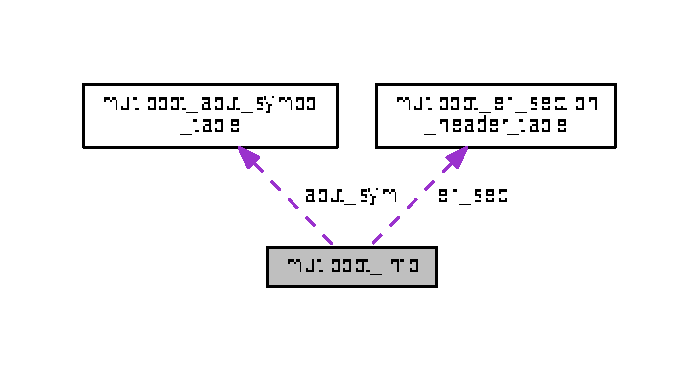
\includegraphics[width=336pt]{structmultiboot__info__coll__graph}
\end{center}
\end{figure}
\subsection*{Public Attributes}
\begin{DoxyCompactItemize}
\item 
\hyperlink{multiboot_8h_a009f355da41fed4badb8a52d432f5186}{multiboot\+\_\+uint32\+\_\+t} \hyperlink{structmultiboot__info_aa562865bc325fd785c9fa4c5056294f3}{flags}
\item 
\hyperlink{multiboot_8h_a009f355da41fed4badb8a52d432f5186}{multiboot\+\_\+uint32\+\_\+t} \hyperlink{structmultiboot__info_aa3503176ee0d132ef98537fa0b36ff09}{mem\+\_\+lower}
\item 
\hyperlink{multiboot_8h_a009f355da41fed4badb8a52d432f5186}{multiboot\+\_\+uint32\+\_\+t} \hyperlink{structmultiboot__info_a87db5803d5a79490b2bf32cb8e9a05c9}{mem\+\_\+upper}
\item 
\hyperlink{multiboot_8h_a009f355da41fed4badb8a52d432f5186}{multiboot\+\_\+uint32\+\_\+t} \hyperlink{structmultiboot__info_ac7dd626a05c9ba62d55ea8a7a254de80}{boot\+\_\+device}
\item 
\hyperlink{multiboot_8h_a009f355da41fed4badb8a52d432f5186}{multiboot\+\_\+uint32\+\_\+t} \hyperlink{structmultiboot__info_a0f2f05f69c69c615bf2b4820d357cf36}{cmdline}
\item 
\hyperlink{multiboot_8h_a009f355da41fed4badb8a52d432f5186}{multiboot\+\_\+uint32\+\_\+t} \hyperlink{structmultiboot__info_aebdafce31f94277d138202f7b1ec35cc}{mods\+\_\+count}
\item 
\hyperlink{multiboot_8h_a009f355da41fed4badb8a52d432f5186}{multiboot\+\_\+uint32\+\_\+t} \hyperlink{structmultiboot__info_a854bdbfa7b23c9c3dfa0bfc155ef8242}{mods\+\_\+addr}
\item 
\begin{tabbing}
xx\=xx\=xx\=xx\=xx\=xx\=xx\=xx\=xx\=\kill
union \{\\
\>\hyperlink{multiboot_8h_a2f11acfde9ee0022a999f69d3e972352}{multiboot\_aout\_symbol\_table\_t} \hyperlink{structmultiboot__info_acf01e96c5d199a398901516df535a5bb}{aout\_sym}\\
\>\hyperlink{multiboot_8h_a2ea4dd45da23724e95b9fc701b41d1e0}{multiboot\_elf\_section\_header\_table\_t} \hyperlink{structmultiboot__info_ab06f895b6b56ca37c8123d145da52387}{elf\_sec}\\
\} \hyperlink{structmultiboot__info_a61dc20144c958a07801f479c74e5867e}{u}\\

\end{tabbing}\item 
\hyperlink{multiboot_8h_a009f355da41fed4badb8a52d432f5186}{multiboot\+\_\+uint32\+\_\+t} \hyperlink{structmultiboot__info_a86a0d881c5233a4b1c8cd690ccd19b75}{mmap\+\_\+length}
\item 
\hyperlink{multiboot_8h_a009f355da41fed4badb8a52d432f5186}{multiboot\+\_\+uint32\+\_\+t} \hyperlink{structmultiboot__info_aacf83273b9f8448d91fb24690492c0d8}{mmap\+\_\+addr}
\item 
\hyperlink{multiboot_8h_a009f355da41fed4badb8a52d432f5186}{multiboot\+\_\+uint32\+\_\+t} \hyperlink{structmultiboot__info_abe859eaa7e97309f072b3bc1caf5742e}{drives\+\_\+length}
\item 
\hyperlink{multiboot_8h_a009f355da41fed4badb8a52d432f5186}{multiboot\+\_\+uint32\+\_\+t} \hyperlink{structmultiboot__info_a34d90ffaaf58124095cb17de9c3b1515}{drives\+\_\+addr}
\item 
\hyperlink{multiboot_8h_a009f355da41fed4badb8a52d432f5186}{multiboot\+\_\+uint32\+\_\+t} \hyperlink{structmultiboot__info_a919ce01f85d05ab90857f8591dfb3948}{config\+\_\+table}
\item 
\hyperlink{multiboot_8h_a009f355da41fed4badb8a52d432f5186}{multiboot\+\_\+uint32\+\_\+t} \hyperlink{structmultiboot__info_a4442438f7c2da9c0cf87a94ffd1acc04}{boot\+\_\+loader\+\_\+name}
\item 
\hyperlink{multiboot_8h_a009f355da41fed4badb8a52d432f5186}{multiboot\+\_\+uint32\+\_\+t} \hyperlink{structmultiboot__info_ad4285d60142d241a9e6b68a03e62ee0a}{apm\+\_\+table}
\item 
\hyperlink{multiboot_8h_a009f355da41fed4badb8a52d432f5186}{multiboot\+\_\+uint32\+\_\+t} \hyperlink{structmultiboot__info_a06191cef73b64e9d64a01850547fd2e8}{vbe\+\_\+control\+\_\+info}
\item 
\hyperlink{multiboot_8h_a009f355da41fed4badb8a52d432f5186}{multiboot\+\_\+uint32\+\_\+t} \hyperlink{structmultiboot__info_a88f574fe1adbcb5ff63fc95b2e072b4c}{vbe\+\_\+mode\+\_\+info}
\item 
\hyperlink{multiboot_8h_a3a11e3c2b5e0617736a05343aa5795b3}{multiboot\+\_\+uint16\+\_\+t} \hyperlink{structmultiboot__info_ac7653182e52bddb7e437cc8a66d74ce5}{vbe\+\_\+mode}
\item 
\hyperlink{multiboot_8h_a3a11e3c2b5e0617736a05343aa5795b3}{multiboot\+\_\+uint16\+\_\+t} \hyperlink{structmultiboot__info_a204c99787efd58c0f54fe1e056b1d69f}{vbe\+\_\+interface\+\_\+seg}
\item 
\hyperlink{multiboot_8h_a3a11e3c2b5e0617736a05343aa5795b3}{multiboot\+\_\+uint16\+\_\+t} \hyperlink{structmultiboot__info_a1621d51b1cc198a1496e9f61b3708291}{vbe\+\_\+interface\+\_\+off}
\item 
\hyperlink{multiboot_8h_a3a11e3c2b5e0617736a05343aa5795b3}{multiboot\+\_\+uint16\+\_\+t} \hyperlink{structmultiboot__info_ab3c537df524db1ed0aeaa2e6f61a23e6}{vbe\+\_\+interface\+\_\+len}
\item 
\hyperlink{multiboot_8h_a8dfdd61648b48aa31845db590970e06a}{multiboot\+\_\+uint64\+\_\+t} \hyperlink{structmultiboot__info_a17bb708a0853e8618cb208b31d21c3c2}{framebuffer\+\_\+addr}
\item 
\hyperlink{multiboot_8h_a009f355da41fed4badb8a52d432f5186}{multiboot\+\_\+uint32\+\_\+t} \hyperlink{structmultiboot__info_a7d96c148c0360ca105ed700de1a8471b}{framebuffer\+\_\+pitch}
\item 
\hyperlink{multiboot_8h_a009f355da41fed4badb8a52d432f5186}{multiboot\+\_\+uint32\+\_\+t} \hyperlink{structmultiboot__info_a72cac058f9f9ed05738d4d1b003424fd}{framebuffer\+\_\+width}
\item 
\hyperlink{multiboot_8h_a009f355da41fed4badb8a52d432f5186}{multiboot\+\_\+uint32\+\_\+t} \hyperlink{structmultiboot__info_adc94f66e25a23bb66053837c1c0ec758}{framebuffer\+\_\+height}
\item 
\hyperlink{multiboot_8h_a037f602538fccf97e90021c19fdfc047}{multiboot\+\_\+uint8\+\_\+t} \hyperlink{structmultiboot__info_a721623c95cf1c95b61678f1e2289893c}{framebuffer\+\_\+bpp}
\item 
\hyperlink{multiboot_8h_a037f602538fccf97e90021c19fdfc047}{multiboot\+\_\+uint8\+\_\+t} \hyperlink{structmultiboot__info_a98b2122e2f14dcfcbfabb018e602fdfc}{framebuffer\+\_\+type}
\item 
\begin{tabbing}
xx\=xx\=xx\=xx\=xx\=xx\=xx\=xx\=xx\=\kill
union \{\\
\>struct \{\\
\>\>\hyperlink{multiboot_8h_a009f355da41fed4badb8a52d432f5186}{multiboot\_uint32\_t} \hyperlink{structmultiboot__info_a3dedc220bb3e97b53f78a72f66d202e1}{framebuffer\_palette\_addr}\\
\>\>\hyperlink{multiboot_8h_a3a11e3c2b5e0617736a05343aa5795b3}{multiboot\_uint16\_t} \hyperlink{structmultiboot__info_a37f9442827e23b75513f41b2e1674f8d}{framebuffer\_palette\_num\_colors}\\
\>\} \\
\>struct \{\\
\>\>\hyperlink{multiboot_8h_a037f602538fccf97e90021c19fdfc047}{multiboot\_uint8\_t} \hyperlink{structmultiboot__info_a0ba9589c99e3d0968e1cfabed744bfa5}{framebuffer\_red\_field\_position}\\
\>\>\hyperlink{multiboot_8h_a037f602538fccf97e90021c19fdfc047}{multiboot\_uint8\_t} \hyperlink{structmultiboot__info_a12b01720d430270e5afc2b28f3318e3d}{framebuffer\_red\_mask\_size}\\
\>\>\hyperlink{multiboot_8h_a037f602538fccf97e90021c19fdfc047}{multiboot\_uint8\_t} \hyperlink{structmultiboot__info_a2fe2ac9812c7ff88c7eeb306bd836fe3}{framebuffer\_green\_field\_position}\\
\>\>\hyperlink{multiboot_8h_a037f602538fccf97e90021c19fdfc047}{multiboot\_uint8\_t} \hyperlink{structmultiboot__info_a18cfe05edd236d9ddbbd3d0118d22e47}{framebuffer\_green\_mask\_size}\\
\>\>\hyperlink{multiboot_8h_a037f602538fccf97e90021c19fdfc047}{multiboot\_uint8\_t} \hyperlink{structmultiboot__info_aef7453a08ec80dcd5f2645bec2995a0f}{framebuffer\_blue\_field\_position}\\
\>\>\hyperlink{multiboot_8h_a037f602538fccf97e90021c19fdfc047}{multiboot\_uint8\_t} \hyperlink{structmultiboot__info_a0409fd6c556aa388c7845a222957e455}{framebuffer\_blue\_mask\_size}\\
\>\} \\
\}; \\

\end{tabbing}\end{DoxyCompactItemize}


\subsection{Member Data Documentation}
\hypertarget{structmultiboot__info_af694b7644759d2f7526a0b9182426207}{}\subsubsection[{"@2}]{\setlength{\rightskip}{0pt plus 5cm}union \{ ... \} }\label{structmultiboot__info_af694b7644759d2f7526a0b9182426207}
\hypertarget{structmultiboot__info_acf01e96c5d199a398901516df535a5bb}{}\index{multiboot\+\_\+info@{multiboot\+\_\+info}!aout\+\_\+sym@{aout\+\_\+sym}}
\index{aout\+\_\+sym@{aout\+\_\+sym}!multiboot\+\_\+info@{multiboot\+\_\+info}}
\subsubsection[{aout\+\_\+sym}]{\setlength{\rightskip}{0pt plus 5cm}{\bf multiboot\+\_\+aout\+\_\+symbol\+\_\+table\+\_\+t} multiboot\+\_\+info\+::aout\+\_\+sym}\label{structmultiboot__info_acf01e96c5d199a398901516df535a5bb}
\hypertarget{structmultiboot__info_ad4285d60142d241a9e6b68a03e62ee0a}{}\index{multiboot\+\_\+info@{multiboot\+\_\+info}!apm\+\_\+table@{apm\+\_\+table}}
\index{apm\+\_\+table@{apm\+\_\+table}!multiboot\+\_\+info@{multiboot\+\_\+info}}
\subsubsection[{apm\+\_\+table}]{\setlength{\rightskip}{0pt plus 5cm}{\bf multiboot\+\_\+uint32\+\_\+t} multiboot\+\_\+info\+::apm\+\_\+table}\label{structmultiboot__info_ad4285d60142d241a9e6b68a03e62ee0a}
\hypertarget{structmultiboot__info_ac7dd626a05c9ba62d55ea8a7a254de80}{}\index{multiboot\+\_\+info@{multiboot\+\_\+info}!boot\+\_\+device@{boot\+\_\+device}}
\index{boot\+\_\+device@{boot\+\_\+device}!multiboot\+\_\+info@{multiboot\+\_\+info}}
\subsubsection[{boot\+\_\+device}]{\setlength{\rightskip}{0pt plus 5cm}{\bf multiboot\+\_\+uint32\+\_\+t} multiboot\+\_\+info\+::boot\+\_\+device}\label{structmultiboot__info_ac7dd626a05c9ba62d55ea8a7a254de80}
\hypertarget{structmultiboot__info_a4442438f7c2da9c0cf87a94ffd1acc04}{}\index{multiboot\+\_\+info@{multiboot\+\_\+info}!boot\+\_\+loader\+\_\+name@{boot\+\_\+loader\+\_\+name}}
\index{boot\+\_\+loader\+\_\+name@{boot\+\_\+loader\+\_\+name}!multiboot\+\_\+info@{multiboot\+\_\+info}}
\subsubsection[{boot\+\_\+loader\+\_\+name}]{\setlength{\rightskip}{0pt plus 5cm}{\bf multiboot\+\_\+uint32\+\_\+t} multiboot\+\_\+info\+::boot\+\_\+loader\+\_\+name}\label{structmultiboot__info_a4442438f7c2da9c0cf87a94ffd1acc04}
\hypertarget{structmultiboot__info_a0f2f05f69c69c615bf2b4820d357cf36}{}\index{multiboot\+\_\+info@{multiboot\+\_\+info}!cmdline@{cmdline}}
\index{cmdline@{cmdline}!multiboot\+\_\+info@{multiboot\+\_\+info}}
\subsubsection[{cmdline}]{\setlength{\rightskip}{0pt plus 5cm}{\bf multiboot\+\_\+uint32\+\_\+t} multiboot\+\_\+info\+::cmdline}\label{structmultiboot__info_a0f2f05f69c69c615bf2b4820d357cf36}
\hypertarget{structmultiboot__info_a919ce01f85d05ab90857f8591dfb3948}{}\index{multiboot\+\_\+info@{multiboot\+\_\+info}!config\+\_\+table@{config\+\_\+table}}
\index{config\+\_\+table@{config\+\_\+table}!multiboot\+\_\+info@{multiboot\+\_\+info}}
\subsubsection[{config\+\_\+table}]{\setlength{\rightskip}{0pt plus 5cm}{\bf multiboot\+\_\+uint32\+\_\+t} multiboot\+\_\+info\+::config\+\_\+table}\label{structmultiboot__info_a919ce01f85d05ab90857f8591dfb3948}
\hypertarget{structmultiboot__info_a34d90ffaaf58124095cb17de9c3b1515}{}\index{multiboot\+\_\+info@{multiboot\+\_\+info}!drives\+\_\+addr@{drives\+\_\+addr}}
\index{drives\+\_\+addr@{drives\+\_\+addr}!multiboot\+\_\+info@{multiboot\+\_\+info}}
\subsubsection[{drives\+\_\+addr}]{\setlength{\rightskip}{0pt plus 5cm}{\bf multiboot\+\_\+uint32\+\_\+t} multiboot\+\_\+info\+::drives\+\_\+addr}\label{structmultiboot__info_a34d90ffaaf58124095cb17de9c3b1515}
\hypertarget{structmultiboot__info_abe859eaa7e97309f072b3bc1caf5742e}{}\index{multiboot\+\_\+info@{multiboot\+\_\+info}!drives\+\_\+length@{drives\+\_\+length}}
\index{drives\+\_\+length@{drives\+\_\+length}!multiboot\+\_\+info@{multiboot\+\_\+info}}
\subsubsection[{drives\+\_\+length}]{\setlength{\rightskip}{0pt plus 5cm}{\bf multiboot\+\_\+uint32\+\_\+t} multiboot\+\_\+info\+::drives\+\_\+length}\label{structmultiboot__info_abe859eaa7e97309f072b3bc1caf5742e}
\hypertarget{structmultiboot__info_ab06f895b6b56ca37c8123d145da52387}{}\index{multiboot\+\_\+info@{multiboot\+\_\+info}!elf\+\_\+sec@{elf\+\_\+sec}}
\index{elf\+\_\+sec@{elf\+\_\+sec}!multiboot\+\_\+info@{multiboot\+\_\+info}}
\subsubsection[{elf\+\_\+sec}]{\setlength{\rightskip}{0pt plus 5cm}{\bf multiboot\+\_\+elf\+\_\+section\+\_\+header\+\_\+table\+\_\+t} multiboot\+\_\+info\+::elf\+\_\+sec}\label{structmultiboot__info_ab06f895b6b56ca37c8123d145da52387}
\hypertarget{structmultiboot__info_aa562865bc325fd785c9fa4c5056294f3}{}\index{multiboot\+\_\+info@{multiboot\+\_\+info}!flags@{flags}}
\index{flags@{flags}!multiboot\+\_\+info@{multiboot\+\_\+info}}
\subsubsection[{flags}]{\setlength{\rightskip}{0pt plus 5cm}{\bf multiboot\+\_\+uint32\+\_\+t} multiboot\+\_\+info\+::flags}\label{structmultiboot__info_aa562865bc325fd785c9fa4c5056294f3}
\hypertarget{structmultiboot__info_a17bb708a0853e8618cb208b31d21c3c2}{}\index{multiboot\+\_\+info@{multiboot\+\_\+info}!framebuffer\+\_\+addr@{framebuffer\+\_\+addr}}
\index{framebuffer\+\_\+addr@{framebuffer\+\_\+addr}!multiboot\+\_\+info@{multiboot\+\_\+info}}
\subsubsection[{framebuffer\+\_\+addr}]{\setlength{\rightskip}{0pt plus 5cm}{\bf multiboot\+\_\+uint64\+\_\+t} multiboot\+\_\+info\+::framebuffer\+\_\+addr}\label{structmultiboot__info_a17bb708a0853e8618cb208b31d21c3c2}
\hypertarget{structmultiboot__info_aef7453a08ec80dcd5f2645bec2995a0f}{}\index{multiboot\+\_\+info@{multiboot\+\_\+info}!framebuffer\+\_\+blue\+\_\+field\+\_\+position@{framebuffer\+\_\+blue\+\_\+field\+\_\+position}}
\index{framebuffer\+\_\+blue\+\_\+field\+\_\+position@{framebuffer\+\_\+blue\+\_\+field\+\_\+position}!multiboot\+\_\+info@{multiboot\+\_\+info}}
\subsubsection[{framebuffer\+\_\+blue\+\_\+field\+\_\+position}]{\setlength{\rightskip}{0pt plus 5cm}{\bf multiboot\+\_\+uint8\+\_\+t} multiboot\+\_\+info\+::framebuffer\+\_\+blue\+\_\+field\+\_\+position}\label{structmultiboot__info_aef7453a08ec80dcd5f2645bec2995a0f}
\hypertarget{structmultiboot__info_a0409fd6c556aa388c7845a222957e455}{}\index{multiboot\+\_\+info@{multiboot\+\_\+info}!framebuffer\+\_\+blue\+\_\+mask\+\_\+size@{framebuffer\+\_\+blue\+\_\+mask\+\_\+size}}
\index{framebuffer\+\_\+blue\+\_\+mask\+\_\+size@{framebuffer\+\_\+blue\+\_\+mask\+\_\+size}!multiboot\+\_\+info@{multiboot\+\_\+info}}
\subsubsection[{framebuffer\+\_\+blue\+\_\+mask\+\_\+size}]{\setlength{\rightskip}{0pt plus 5cm}{\bf multiboot\+\_\+uint8\+\_\+t} multiboot\+\_\+info\+::framebuffer\+\_\+blue\+\_\+mask\+\_\+size}\label{structmultiboot__info_a0409fd6c556aa388c7845a222957e455}
\hypertarget{structmultiboot__info_a721623c95cf1c95b61678f1e2289893c}{}\index{multiboot\+\_\+info@{multiboot\+\_\+info}!framebuffer\+\_\+bpp@{framebuffer\+\_\+bpp}}
\index{framebuffer\+\_\+bpp@{framebuffer\+\_\+bpp}!multiboot\+\_\+info@{multiboot\+\_\+info}}
\subsubsection[{framebuffer\+\_\+bpp}]{\setlength{\rightskip}{0pt plus 5cm}{\bf multiboot\+\_\+uint8\+\_\+t} multiboot\+\_\+info\+::framebuffer\+\_\+bpp}\label{structmultiboot__info_a721623c95cf1c95b61678f1e2289893c}
\hypertarget{structmultiboot__info_a2fe2ac9812c7ff88c7eeb306bd836fe3}{}\index{multiboot\+\_\+info@{multiboot\+\_\+info}!framebuffer\+\_\+green\+\_\+field\+\_\+position@{framebuffer\+\_\+green\+\_\+field\+\_\+position}}
\index{framebuffer\+\_\+green\+\_\+field\+\_\+position@{framebuffer\+\_\+green\+\_\+field\+\_\+position}!multiboot\+\_\+info@{multiboot\+\_\+info}}
\subsubsection[{framebuffer\+\_\+green\+\_\+field\+\_\+position}]{\setlength{\rightskip}{0pt plus 5cm}{\bf multiboot\+\_\+uint8\+\_\+t} multiboot\+\_\+info\+::framebuffer\+\_\+green\+\_\+field\+\_\+position}\label{structmultiboot__info_a2fe2ac9812c7ff88c7eeb306bd836fe3}
\hypertarget{structmultiboot__info_a18cfe05edd236d9ddbbd3d0118d22e47}{}\index{multiboot\+\_\+info@{multiboot\+\_\+info}!framebuffer\+\_\+green\+\_\+mask\+\_\+size@{framebuffer\+\_\+green\+\_\+mask\+\_\+size}}
\index{framebuffer\+\_\+green\+\_\+mask\+\_\+size@{framebuffer\+\_\+green\+\_\+mask\+\_\+size}!multiboot\+\_\+info@{multiboot\+\_\+info}}
\subsubsection[{framebuffer\+\_\+green\+\_\+mask\+\_\+size}]{\setlength{\rightskip}{0pt plus 5cm}{\bf multiboot\+\_\+uint8\+\_\+t} multiboot\+\_\+info\+::framebuffer\+\_\+green\+\_\+mask\+\_\+size}\label{structmultiboot__info_a18cfe05edd236d9ddbbd3d0118d22e47}
\hypertarget{structmultiboot__info_adc94f66e25a23bb66053837c1c0ec758}{}\index{multiboot\+\_\+info@{multiboot\+\_\+info}!framebuffer\+\_\+height@{framebuffer\+\_\+height}}
\index{framebuffer\+\_\+height@{framebuffer\+\_\+height}!multiboot\+\_\+info@{multiboot\+\_\+info}}
\subsubsection[{framebuffer\+\_\+height}]{\setlength{\rightskip}{0pt plus 5cm}{\bf multiboot\+\_\+uint32\+\_\+t} multiboot\+\_\+info\+::framebuffer\+\_\+height}\label{structmultiboot__info_adc94f66e25a23bb66053837c1c0ec758}
\hypertarget{structmultiboot__info_a3dedc220bb3e97b53f78a72f66d202e1}{}\index{multiboot\+\_\+info@{multiboot\+\_\+info}!framebuffer\+\_\+palette\+\_\+addr@{framebuffer\+\_\+palette\+\_\+addr}}
\index{framebuffer\+\_\+palette\+\_\+addr@{framebuffer\+\_\+palette\+\_\+addr}!multiboot\+\_\+info@{multiboot\+\_\+info}}
\subsubsection[{framebuffer\+\_\+palette\+\_\+addr}]{\setlength{\rightskip}{0pt plus 5cm}{\bf multiboot\+\_\+uint32\+\_\+t} multiboot\+\_\+info\+::framebuffer\+\_\+palette\+\_\+addr}\label{structmultiboot__info_a3dedc220bb3e97b53f78a72f66d202e1}
\hypertarget{structmultiboot__info_a37f9442827e23b75513f41b2e1674f8d}{}\index{multiboot\+\_\+info@{multiboot\+\_\+info}!framebuffer\+\_\+palette\+\_\+num\+\_\+colors@{framebuffer\+\_\+palette\+\_\+num\+\_\+colors}}
\index{framebuffer\+\_\+palette\+\_\+num\+\_\+colors@{framebuffer\+\_\+palette\+\_\+num\+\_\+colors}!multiboot\+\_\+info@{multiboot\+\_\+info}}
\subsubsection[{framebuffer\+\_\+palette\+\_\+num\+\_\+colors}]{\setlength{\rightskip}{0pt plus 5cm}{\bf multiboot\+\_\+uint16\+\_\+t} multiboot\+\_\+info\+::framebuffer\+\_\+palette\+\_\+num\+\_\+colors}\label{structmultiboot__info_a37f9442827e23b75513f41b2e1674f8d}
\hypertarget{structmultiboot__info_a7d96c148c0360ca105ed700de1a8471b}{}\index{multiboot\+\_\+info@{multiboot\+\_\+info}!framebuffer\+\_\+pitch@{framebuffer\+\_\+pitch}}
\index{framebuffer\+\_\+pitch@{framebuffer\+\_\+pitch}!multiboot\+\_\+info@{multiboot\+\_\+info}}
\subsubsection[{framebuffer\+\_\+pitch}]{\setlength{\rightskip}{0pt plus 5cm}{\bf multiboot\+\_\+uint32\+\_\+t} multiboot\+\_\+info\+::framebuffer\+\_\+pitch}\label{structmultiboot__info_a7d96c148c0360ca105ed700de1a8471b}
\hypertarget{structmultiboot__info_a0ba9589c99e3d0968e1cfabed744bfa5}{}\index{multiboot\+\_\+info@{multiboot\+\_\+info}!framebuffer\+\_\+red\+\_\+field\+\_\+position@{framebuffer\+\_\+red\+\_\+field\+\_\+position}}
\index{framebuffer\+\_\+red\+\_\+field\+\_\+position@{framebuffer\+\_\+red\+\_\+field\+\_\+position}!multiboot\+\_\+info@{multiboot\+\_\+info}}
\subsubsection[{framebuffer\+\_\+red\+\_\+field\+\_\+position}]{\setlength{\rightskip}{0pt plus 5cm}{\bf multiboot\+\_\+uint8\+\_\+t} multiboot\+\_\+info\+::framebuffer\+\_\+red\+\_\+field\+\_\+position}\label{structmultiboot__info_a0ba9589c99e3d0968e1cfabed744bfa5}
\hypertarget{structmultiboot__info_a12b01720d430270e5afc2b28f3318e3d}{}\index{multiboot\+\_\+info@{multiboot\+\_\+info}!framebuffer\+\_\+red\+\_\+mask\+\_\+size@{framebuffer\+\_\+red\+\_\+mask\+\_\+size}}
\index{framebuffer\+\_\+red\+\_\+mask\+\_\+size@{framebuffer\+\_\+red\+\_\+mask\+\_\+size}!multiboot\+\_\+info@{multiboot\+\_\+info}}
\subsubsection[{framebuffer\+\_\+red\+\_\+mask\+\_\+size}]{\setlength{\rightskip}{0pt plus 5cm}{\bf multiboot\+\_\+uint8\+\_\+t} multiboot\+\_\+info\+::framebuffer\+\_\+red\+\_\+mask\+\_\+size}\label{structmultiboot__info_a12b01720d430270e5afc2b28f3318e3d}
\hypertarget{structmultiboot__info_a98b2122e2f14dcfcbfabb018e602fdfc}{}\index{multiboot\+\_\+info@{multiboot\+\_\+info}!framebuffer\+\_\+type@{framebuffer\+\_\+type}}
\index{framebuffer\+\_\+type@{framebuffer\+\_\+type}!multiboot\+\_\+info@{multiboot\+\_\+info}}
\subsubsection[{framebuffer\+\_\+type}]{\setlength{\rightskip}{0pt plus 5cm}{\bf multiboot\+\_\+uint8\+\_\+t} multiboot\+\_\+info\+::framebuffer\+\_\+type}\label{structmultiboot__info_a98b2122e2f14dcfcbfabb018e602fdfc}
\hypertarget{structmultiboot__info_a72cac058f9f9ed05738d4d1b003424fd}{}\index{multiboot\+\_\+info@{multiboot\+\_\+info}!framebuffer\+\_\+width@{framebuffer\+\_\+width}}
\index{framebuffer\+\_\+width@{framebuffer\+\_\+width}!multiboot\+\_\+info@{multiboot\+\_\+info}}
\subsubsection[{framebuffer\+\_\+width}]{\setlength{\rightskip}{0pt plus 5cm}{\bf multiboot\+\_\+uint32\+\_\+t} multiboot\+\_\+info\+::framebuffer\+\_\+width}\label{structmultiboot__info_a72cac058f9f9ed05738d4d1b003424fd}
\hypertarget{structmultiboot__info_aa3503176ee0d132ef98537fa0b36ff09}{}\index{multiboot\+\_\+info@{multiboot\+\_\+info}!mem\+\_\+lower@{mem\+\_\+lower}}
\index{mem\+\_\+lower@{mem\+\_\+lower}!multiboot\+\_\+info@{multiboot\+\_\+info}}
\subsubsection[{mem\+\_\+lower}]{\setlength{\rightskip}{0pt plus 5cm}{\bf multiboot\+\_\+uint32\+\_\+t} multiboot\+\_\+info\+::mem\+\_\+lower}\label{structmultiboot__info_aa3503176ee0d132ef98537fa0b36ff09}
\hypertarget{structmultiboot__info_a87db5803d5a79490b2bf32cb8e9a05c9}{}\index{multiboot\+\_\+info@{multiboot\+\_\+info}!mem\+\_\+upper@{mem\+\_\+upper}}
\index{mem\+\_\+upper@{mem\+\_\+upper}!multiboot\+\_\+info@{multiboot\+\_\+info}}
\subsubsection[{mem\+\_\+upper}]{\setlength{\rightskip}{0pt plus 5cm}{\bf multiboot\+\_\+uint32\+\_\+t} multiboot\+\_\+info\+::mem\+\_\+upper}\label{structmultiboot__info_a87db5803d5a79490b2bf32cb8e9a05c9}
\hypertarget{structmultiboot__info_aacf83273b9f8448d91fb24690492c0d8}{}\index{multiboot\+\_\+info@{multiboot\+\_\+info}!mmap\+\_\+addr@{mmap\+\_\+addr}}
\index{mmap\+\_\+addr@{mmap\+\_\+addr}!multiboot\+\_\+info@{multiboot\+\_\+info}}
\subsubsection[{mmap\+\_\+addr}]{\setlength{\rightskip}{0pt plus 5cm}{\bf multiboot\+\_\+uint32\+\_\+t} multiboot\+\_\+info\+::mmap\+\_\+addr}\label{structmultiboot__info_aacf83273b9f8448d91fb24690492c0d8}
\hypertarget{structmultiboot__info_a86a0d881c5233a4b1c8cd690ccd19b75}{}\index{multiboot\+\_\+info@{multiboot\+\_\+info}!mmap\+\_\+length@{mmap\+\_\+length}}
\index{mmap\+\_\+length@{mmap\+\_\+length}!multiboot\+\_\+info@{multiboot\+\_\+info}}
\subsubsection[{mmap\+\_\+length}]{\setlength{\rightskip}{0pt plus 5cm}{\bf multiboot\+\_\+uint32\+\_\+t} multiboot\+\_\+info\+::mmap\+\_\+length}\label{structmultiboot__info_a86a0d881c5233a4b1c8cd690ccd19b75}
\hypertarget{structmultiboot__info_a854bdbfa7b23c9c3dfa0bfc155ef8242}{}\index{multiboot\+\_\+info@{multiboot\+\_\+info}!mods\+\_\+addr@{mods\+\_\+addr}}
\index{mods\+\_\+addr@{mods\+\_\+addr}!multiboot\+\_\+info@{multiboot\+\_\+info}}
\subsubsection[{mods\+\_\+addr}]{\setlength{\rightskip}{0pt plus 5cm}{\bf multiboot\+\_\+uint32\+\_\+t} multiboot\+\_\+info\+::mods\+\_\+addr}\label{structmultiboot__info_a854bdbfa7b23c9c3dfa0bfc155ef8242}
\hypertarget{structmultiboot__info_aebdafce31f94277d138202f7b1ec35cc}{}\index{multiboot\+\_\+info@{multiboot\+\_\+info}!mods\+\_\+count@{mods\+\_\+count}}
\index{mods\+\_\+count@{mods\+\_\+count}!multiboot\+\_\+info@{multiboot\+\_\+info}}
\subsubsection[{mods\+\_\+count}]{\setlength{\rightskip}{0pt plus 5cm}{\bf multiboot\+\_\+uint32\+\_\+t} multiboot\+\_\+info\+::mods\+\_\+count}\label{structmultiboot__info_aebdafce31f94277d138202f7b1ec35cc}
\hypertarget{structmultiboot__info_a61dc20144c958a07801f479c74e5867e}{}\index{multiboot\+\_\+info@{multiboot\+\_\+info}!u@{u}}
\index{u@{u}!multiboot\+\_\+info@{multiboot\+\_\+info}}
\subsubsection[{u}]{\setlength{\rightskip}{0pt plus 5cm}union \{ ... \}   multiboot\+\_\+info\+::u}\label{structmultiboot__info_a61dc20144c958a07801f479c74e5867e}
\hypertarget{structmultiboot__info_a06191cef73b64e9d64a01850547fd2e8}{}\index{multiboot\+\_\+info@{multiboot\+\_\+info}!vbe\+\_\+control\+\_\+info@{vbe\+\_\+control\+\_\+info}}
\index{vbe\+\_\+control\+\_\+info@{vbe\+\_\+control\+\_\+info}!multiboot\+\_\+info@{multiboot\+\_\+info}}
\subsubsection[{vbe\+\_\+control\+\_\+info}]{\setlength{\rightskip}{0pt plus 5cm}{\bf multiboot\+\_\+uint32\+\_\+t} multiboot\+\_\+info\+::vbe\+\_\+control\+\_\+info}\label{structmultiboot__info_a06191cef73b64e9d64a01850547fd2e8}
\hypertarget{structmultiboot__info_ab3c537df524db1ed0aeaa2e6f61a23e6}{}\index{multiboot\+\_\+info@{multiboot\+\_\+info}!vbe\+\_\+interface\+\_\+len@{vbe\+\_\+interface\+\_\+len}}
\index{vbe\+\_\+interface\+\_\+len@{vbe\+\_\+interface\+\_\+len}!multiboot\+\_\+info@{multiboot\+\_\+info}}
\subsubsection[{vbe\+\_\+interface\+\_\+len}]{\setlength{\rightskip}{0pt plus 5cm}{\bf multiboot\+\_\+uint16\+\_\+t} multiboot\+\_\+info\+::vbe\+\_\+interface\+\_\+len}\label{structmultiboot__info_ab3c537df524db1ed0aeaa2e6f61a23e6}
\hypertarget{structmultiboot__info_a1621d51b1cc198a1496e9f61b3708291}{}\index{multiboot\+\_\+info@{multiboot\+\_\+info}!vbe\+\_\+interface\+\_\+off@{vbe\+\_\+interface\+\_\+off}}
\index{vbe\+\_\+interface\+\_\+off@{vbe\+\_\+interface\+\_\+off}!multiboot\+\_\+info@{multiboot\+\_\+info}}
\subsubsection[{vbe\+\_\+interface\+\_\+off}]{\setlength{\rightskip}{0pt plus 5cm}{\bf multiboot\+\_\+uint16\+\_\+t} multiboot\+\_\+info\+::vbe\+\_\+interface\+\_\+off}\label{structmultiboot__info_a1621d51b1cc198a1496e9f61b3708291}
\hypertarget{structmultiboot__info_a204c99787efd58c0f54fe1e056b1d69f}{}\index{multiboot\+\_\+info@{multiboot\+\_\+info}!vbe\+\_\+interface\+\_\+seg@{vbe\+\_\+interface\+\_\+seg}}
\index{vbe\+\_\+interface\+\_\+seg@{vbe\+\_\+interface\+\_\+seg}!multiboot\+\_\+info@{multiboot\+\_\+info}}
\subsubsection[{vbe\+\_\+interface\+\_\+seg}]{\setlength{\rightskip}{0pt plus 5cm}{\bf multiboot\+\_\+uint16\+\_\+t} multiboot\+\_\+info\+::vbe\+\_\+interface\+\_\+seg}\label{structmultiboot__info_a204c99787efd58c0f54fe1e056b1d69f}
\hypertarget{structmultiboot__info_ac7653182e52bddb7e437cc8a66d74ce5}{}\index{multiboot\+\_\+info@{multiboot\+\_\+info}!vbe\+\_\+mode@{vbe\+\_\+mode}}
\index{vbe\+\_\+mode@{vbe\+\_\+mode}!multiboot\+\_\+info@{multiboot\+\_\+info}}
\subsubsection[{vbe\+\_\+mode}]{\setlength{\rightskip}{0pt plus 5cm}{\bf multiboot\+\_\+uint16\+\_\+t} multiboot\+\_\+info\+::vbe\+\_\+mode}\label{structmultiboot__info_ac7653182e52bddb7e437cc8a66d74ce5}
\hypertarget{structmultiboot__info_a88f574fe1adbcb5ff63fc95b2e072b4c}{}\index{multiboot\+\_\+info@{multiboot\+\_\+info}!vbe\+\_\+mode\+\_\+info@{vbe\+\_\+mode\+\_\+info}}
\index{vbe\+\_\+mode\+\_\+info@{vbe\+\_\+mode\+\_\+info}!multiboot\+\_\+info@{multiboot\+\_\+info}}
\subsubsection[{vbe\+\_\+mode\+\_\+info}]{\setlength{\rightskip}{0pt plus 5cm}{\bf multiboot\+\_\+uint32\+\_\+t} multiboot\+\_\+info\+::vbe\+\_\+mode\+\_\+info}\label{structmultiboot__info_a88f574fe1adbcb5ff63fc95b2e072b4c}


The documentation for this struct was generated from the following file\+:\begin{DoxyCompactItemize}
\item 
boot/x86/\hyperlink{multiboot_8h}{multiboot.\+h}\end{DoxyCompactItemize}

\hypertarget{structmultiboot__mmap__entry}{}\section{multiboot\+\_\+mmap\+\_\+entry Struct Reference}
\label{structmultiboot__mmap__entry}\index{multiboot\+\_\+mmap\+\_\+entry@{multiboot\+\_\+mmap\+\_\+entry}}


{\ttfamily \#include $<$multiboot.\+h$>$}

\subsection*{Public Attributes}
\begin{DoxyCompactItemize}
\item 
\hyperlink{multiboot_8h_a009f355da41fed4badb8a52d432f5186}{multiboot\+\_\+uint32\+\_\+t} \hyperlink{structmultiboot__mmap__entry_af10c1835051b4b08bdcdb538c1b4101d}{size}
\item 
\hyperlink{multiboot_8h_a8dfdd61648b48aa31845db590970e06a}{multiboot\+\_\+uint64\+\_\+t} \hyperlink{structmultiboot__mmap__entry_a3f76a637264b83e30967bcd808ff403c}{addr}
\item 
\hyperlink{multiboot_8h_a8dfdd61648b48aa31845db590970e06a}{multiboot\+\_\+uint64\+\_\+t} \hyperlink{structmultiboot__mmap__entry_a6bfa44919a328492fa4e3d6239a23352}{len}
\item 
\hyperlink{multiboot_8h_a009f355da41fed4badb8a52d432f5186}{multiboot\+\_\+uint32\+\_\+t} \hyperlink{structmultiboot__mmap__entry_aa6fc447c57f074d0babfe3bbb7017de9}{type}
\end{DoxyCompactItemize}


\subsection{Member Data Documentation}
\hypertarget{structmultiboot__mmap__entry_a3f76a637264b83e30967bcd808ff403c}{}\index{multiboot\+\_\+mmap\+\_\+entry@{multiboot\+\_\+mmap\+\_\+entry}!addr@{addr}}
\index{addr@{addr}!multiboot\+\_\+mmap\+\_\+entry@{multiboot\+\_\+mmap\+\_\+entry}}
\subsubsection[{addr}]{\setlength{\rightskip}{0pt plus 5cm}{\bf multiboot\+\_\+uint64\+\_\+t} multiboot\+\_\+mmap\+\_\+entry\+::addr}\label{structmultiboot__mmap__entry_a3f76a637264b83e30967bcd808ff403c}
\hypertarget{structmultiboot__mmap__entry_a6bfa44919a328492fa4e3d6239a23352}{}\index{multiboot\+\_\+mmap\+\_\+entry@{multiboot\+\_\+mmap\+\_\+entry}!len@{len}}
\index{len@{len}!multiboot\+\_\+mmap\+\_\+entry@{multiboot\+\_\+mmap\+\_\+entry}}
\subsubsection[{len}]{\setlength{\rightskip}{0pt plus 5cm}{\bf multiboot\+\_\+uint64\+\_\+t} multiboot\+\_\+mmap\+\_\+entry\+::len}\label{structmultiboot__mmap__entry_a6bfa44919a328492fa4e3d6239a23352}
\hypertarget{structmultiboot__mmap__entry_af10c1835051b4b08bdcdb538c1b4101d}{}\index{multiboot\+\_\+mmap\+\_\+entry@{multiboot\+\_\+mmap\+\_\+entry}!size@{size}}
\index{size@{size}!multiboot\+\_\+mmap\+\_\+entry@{multiboot\+\_\+mmap\+\_\+entry}}
\subsubsection[{size}]{\setlength{\rightskip}{0pt plus 5cm}{\bf multiboot\+\_\+uint32\+\_\+t} multiboot\+\_\+mmap\+\_\+entry\+::size}\label{structmultiboot__mmap__entry_af10c1835051b4b08bdcdb538c1b4101d}
\hypertarget{structmultiboot__mmap__entry_aa6fc447c57f074d0babfe3bbb7017de9}{}\index{multiboot\+\_\+mmap\+\_\+entry@{multiboot\+\_\+mmap\+\_\+entry}!type@{type}}
\index{type@{type}!multiboot\+\_\+mmap\+\_\+entry@{multiboot\+\_\+mmap\+\_\+entry}}
\subsubsection[{type}]{\setlength{\rightskip}{0pt plus 5cm}{\bf multiboot\+\_\+uint32\+\_\+t} multiboot\+\_\+mmap\+\_\+entry\+::type}\label{structmultiboot__mmap__entry_aa6fc447c57f074d0babfe3bbb7017de9}


The documentation for this struct was generated from the following file\+:\begin{DoxyCompactItemize}
\item 
boot/x86/\hyperlink{multiboot_8h}{multiboot.\+h}\end{DoxyCompactItemize}

\hypertarget{structmultiboot__mod__list}{}\section{multiboot\+\_\+mod\+\_\+list Struct Reference}
\label{structmultiboot__mod__list}\index{multiboot\+\_\+mod\+\_\+list@{multiboot\+\_\+mod\+\_\+list}}


{\ttfamily \#include $<$multiboot.\+h$>$}

\subsection*{Public Attributes}
\begin{DoxyCompactItemize}
\item 
\hyperlink{multiboot_8h_a009f355da41fed4badb8a52d432f5186}{multiboot\+\_\+uint32\+\_\+t} \hyperlink{structmultiboot__mod__list_afe0e2af1e8c0297c17a7771bd1a62e0f}{mod\+\_\+start}
\item 
\hyperlink{multiboot_8h_a009f355da41fed4badb8a52d432f5186}{multiboot\+\_\+uint32\+\_\+t} \hyperlink{structmultiboot__mod__list_a75b0899f1e1f90d4ff629b7136f5b988}{mod\+\_\+end}
\item 
\hyperlink{multiboot_8h_a009f355da41fed4badb8a52d432f5186}{multiboot\+\_\+uint32\+\_\+t} \hyperlink{structmultiboot__mod__list_a31365a9d2d0cae071f5cb8bddb9b33fb}{cmdline}
\item 
\hyperlink{multiboot_8h_a009f355da41fed4badb8a52d432f5186}{multiboot\+\_\+uint32\+\_\+t} \hyperlink{structmultiboot__mod__list_a63d98e6d313098a4d35b828e204a4e0c}{pad}
\end{DoxyCompactItemize}


\subsection{Member Data Documentation}
\hypertarget{structmultiboot__mod__list_a31365a9d2d0cae071f5cb8bddb9b33fb}{}\index{multiboot\+\_\+mod\+\_\+list@{multiboot\+\_\+mod\+\_\+list}!cmdline@{cmdline}}
\index{cmdline@{cmdline}!multiboot\+\_\+mod\+\_\+list@{multiboot\+\_\+mod\+\_\+list}}
\subsubsection[{cmdline}]{\setlength{\rightskip}{0pt plus 5cm}{\bf multiboot\+\_\+uint32\+\_\+t} multiboot\+\_\+mod\+\_\+list\+::cmdline}\label{structmultiboot__mod__list_a31365a9d2d0cae071f5cb8bddb9b33fb}
\hypertarget{structmultiboot__mod__list_a75b0899f1e1f90d4ff629b7136f5b988}{}\index{multiboot\+\_\+mod\+\_\+list@{multiboot\+\_\+mod\+\_\+list}!mod\+\_\+end@{mod\+\_\+end}}
\index{mod\+\_\+end@{mod\+\_\+end}!multiboot\+\_\+mod\+\_\+list@{multiboot\+\_\+mod\+\_\+list}}
\subsubsection[{mod\+\_\+end}]{\setlength{\rightskip}{0pt plus 5cm}{\bf multiboot\+\_\+uint32\+\_\+t} multiboot\+\_\+mod\+\_\+list\+::mod\+\_\+end}\label{structmultiboot__mod__list_a75b0899f1e1f90d4ff629b7136f5b988}
\hypertarget{structmultiboot__mod__list_afe0e2af1e8c0297c17a7771bd1a62e0f}{}\index{multiboot\+\_\+mod\+\_\+list@{multiboot\+\_\+mod\+\_\+list}!mod\+\_\+start@{mod\+\_\+start}}
\index{mod\+\_\+start@{mod\+\_\+start}!multiboot\+\_\+mod\+\_\+list@{multiboot\+\_\+mod\+\_\+list}}
\subsubsection[{mod\+\_\+start}]{\setlength{\rightskip}{0pt plus 5cm}{\bf multiboot\+\_\+uint32\+\_\+t} multiboot\+\_\+mod\+\_\+list\+::mod\+\_\+start}\label{structmultiboot__mod__list_afe0e2af1e8c0297c17a7771bd1a62e0f}
\hypertarget{structmultiboot__mod__list_a63d98e6d313098a4d35b828e204a4e0c}{}\index{multiboot\+\_\+mod\+\_\+list@{multiboot\+\_\+mod\+\_\+list}!pad@{pad}}
\index{pad@{pad}!multiboot\+\_\+mod\+\_\+list@{multiboot\+\_\+mod\+\_\+list}}
\subsubsection[{pad}]{\setlength{\rightskip}{0pt plus 5cm}{\bf multiboot\+\_\+uint32\+\_\+t} multiboot\+\_\+mod\+\_\+list\+::pad}\label{structmultiboot__mod__list_a63d98e6d313098a4d35b828e204a4e0c}


The documentation for this struct was generated from the following file\+:\begin{DoxyCompactItemize}
\item 
boot/x86/\hyperlink{multiboot_8h}{multiboot.\+h}\end{DoxyCompactItemize}

\hypertarget{class_m_t_gos_1_1_base_1_1_output}{}\section{M\+T\+Gos\+:\+:Base\+:\+:Output Class Reference}
\label{class_m_t_gos_1_1_base_1_1_output}\index{M\+T\+Gos\+::\+Base\+::\+Output@{M\+T\+Gos\+::\+Base\+::\+Output}}


\hyperlink{namespace_m_t_gos_1_1_base}{Base} class for output classes.  




{\ttfamily \#include $<$output.\+hpp$>$}

\subsection*{Public Member Functions}
\begin{DoxyCompactItemize}
\item 
auto \hyperlink{class_m_t_gos_1_1_base_1_1_output_a484df9ac6db83924c80118154f7088a1}{puts} (const char $\ast$) -\/$>$ void
\begin{DoxyCompactList}\small\item\em Outputs an generic null-\/terminated A\+S\+C\+I\+I string. \end{DoxyCompactList}\item 
{\footnotesize template$<$typename T $>$ }\\auto \hyperlink{class_m_t_gos_1_1_base_1_1_output_a6144d124dcb9299c2b95963b8ac7ad54}{operator$<$$<$} (T \&object) -\/$>$ \hyperlink{class_m_t_gos_1_1_base_1_1_output}{Output} \&
\begin{DoxyCompactList}\small\item\em Outputs an object of any type. \end{DoxyCompactList}\end{DoxyCompactItemize}
\subsection*{Private Member Functions}
\begin{DoxyCompactItemize}
\item 
virtual auto \hyperlink{class_m_t_gos_1_1_base_1_1_output_a9e3a286afa694700d5cf7666cf22d2e8}{put\+Char} (int) -\/$>$ void=0
\begin{DoxyCompactList}\small\item\em \hyperlink{class_m_t_gos_1_1_base_1_1_output}{Output} of a character (U\+T\+F-\/32) \end{DoxyCompactList}\item 
auto \hyperlink{class_m_t_gos_1_1_base_1_1_output_a203883edb598ced80d97be427ad07dbe}{put\+Char} (char) -\/$>$ void
\begin{DoxyCompactList}\small\item\em \hyperlink{class_m_t_gos_1_1_base_1_1_output}{Output} of an A\+S\+C\+I\+I-\/char. \end{DoxyCompactList}\end{DoxyCompactItemize}
\subsection*{Private Attributes}
\begin{DoxyCompactItemize}
\item 
int \hyperlink{class_m_t_gos_1_1_base_1_1_output_a1b713f91402dd5c1fa466268fac2e439}{base} =10
\begin{DoxyCompactList}\small\item\em Contains the base stored for number output. \end{DoxyCompactList}\end{DoxyCompactItemize}


\subsection{Detailed Description}
\hyperlink{namespace_m_t_gos_1_1_base}{Base} class for output classes. 

\subsection{Member Function Documentation}
\hypertarget{class_m_t_gos_1_1_base_1_1_output_a6144d124dcb9299c2b95963b8ac7ad54}{}\index{M\+T\+Gos\+::\+Base\+::\+Output@{M\+T\+Gos\+::\+Base\+::\+Output}!operator$<$$<$@{operator$<$$<$}}
\index{operator$<$$<$@{operator$<$$<$}!M\+T\+Gos\+::\+Base\+::\+Output@{M\+T\+Gos\+::\+Base\+::\+Output}}
\subsubsection[{operator$<$$<$(\+T \&object) -\/$>$ Output \&}]{\setlength{\rightskip}{0pt plus 5cm}template$<$typename T $>$ auto M\+T\+Gos\+::\+Base\+::\+Output\+::operator$<$$<$ (
\begin{DoxyParamCaption}
\item[{T \&}]{object}
\end{DoxyParamCaption}
) -\/$>$ {\bf Output} \& \hspace{0.3cm}{\ttfamily [inline]}}\label{class_m_t_gos_1_1_base_1_1_output_a6144d124dcb9299c2b95963b8ac7ad54}


Outputs an object of any type. 



Here is the call graph for this function\+:
\nopagebreak
\begin{figure}[H]
\begin{center}
\leavevmode
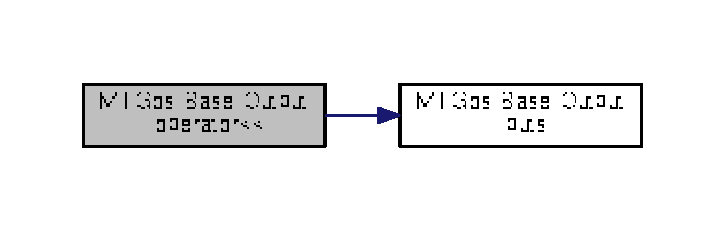
\includegraphics[width=348pt]{class_m_t_gos_1_1_base_1_1_output_a6144d124dcb9299c2b95963b8ac7ad54_cgraph}
\end{center}
\end{figure}


\hypertarget{class_m_t_gos_1_1_base_1_1_output_a9e3a286afa694700d5cf7666cf22d2e8}{}\index{M\+T\+Gos\+::\+Base\+::\+Output@{M\+T\+Gos\+::\+Base\+::\+Output}!put\+Char@{put\+Char}}
\index{put\+Char@{put\+Char}!M\+T\+Gos\+::\+Base\+::\+Output@{M\+T\+Gos\+::\+Base\+::\+Output}}
\subsubsection[{put\+Char(int) -\/$>$ void=0}]{\setlength{\rightskip}{0pt plus 5cm}virtual auto M\+T\+Gos\+::\+Base\+::\+Output\+::put\+Char (
\begin{DoxyParamCaption}
\item[{int}]{}
\end{DoxyParamCaption}
) -\/$>$  void\hspace{0.3cm}{\ttfamily [private]}, {\ttfamily [pure virtual]}}\label{class_m_t_gos_1_1_base_1_1_output_a9e3a286afa694700d5cf7666cf22d2e8}


\hyperlink{class_m_t_gos_1_1_base_1_1_output}{Output} of a character (U\+T\+F-\/32) 

\hypertarget{class_m_t_gos_1_1_base_1_1_output_a203883edb598ced80d97be427ad07dbe}{}\index{M\+T\+Gos\+::\+Base\+::\+Output@{M\+T\+Gos\+::\+Base\+::\+Output}!put\+Char@{put\+Char}}
\index{put\+Char@{put\+Char}!M\+T\+Gos\+::\+Base\+::\+Output@{M\+T\+Gos\+::\+Base\+::\+Output}}
\subsubsection[{put\+Char(char) -\/$>$ void}]{\setlength{\rightskip}{0pt plus 5cm}auto M\+T\+Gos\+::\+Base\+::\+Output\+::put\+Char (
\begin{DoxyParamCaption}
\item[{char}]{}
\end{DoxyParamCaption}
) -\/$>$  void\hspace{0.3cm}{\ttfamily [private]}}\label{class_m_t_gos_1_1_base_1_1_output_a203883edb598ced80d97be427ad07dbe}


\hyperlink{class_m_t_gos_1_1_base_1_1_output}{Output} of an A\+S\+C\+I\+I-\/char. 

\hypertarget{class_m_t_gos_1_1_base_1_1_output_a484df9ac6db83924c80118154f7088a1}{}\index{M\+T\+Gos\+::\+Base\+::\+Output@{M\+T\+Gos\+::\+Base\+::\+Output}!puts@{puts}}
\index{puts@{puts}!M\+T\+Gos\+::\+Base\+::\+Output@{M\+T\+Gos\+::\+Base\+::\+Output}}
\subsubsection[{puts(const char $\ast$) -\/$>$ void}]{\setlength{\rightskip}{0pt plus 5cm}auto M\+T\+Gos\+::\+Base\+::\+Output\+::puts (
\begin{DoxyParamCaption}
\item[{const char $\ast$}]{}
\end{DoxyParamCaption}
) -\/$>$  void}\label{class_m_t_gos_1_1_base_1_1_output_a484df9ac6db83924c80118154f7088a1}


Outputs an generic null-\/terminated A\+S\+C\+I\+I string. 



Here is the caller graph for this function\+:
\nopagebreak
\begin{figure}[H]
\begin{center}
\leavevmode
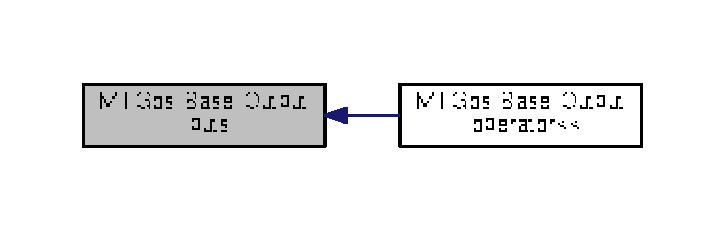
\includegraphics[width=348pt]{class_m_t_gos_1_1_base_1_1_output_a484df9ac6db83924c80118154f7088a1_icgraph}
\end{center}
\end{figure}




\subsection{Member Data Documentation}
\hypertarget{class_m_t_gos_1_1_base_1_1_output_a1b713f91402dd5c1fa466268fac2e439}{}\index{M\+T\+Gos\+::\+Base\+::\+Output@{M\+T\+Gos\+::\+Base\+::\+Output}!base@{base}}
\index{base@{base}!M\+T\+Gos\+::\+Base\+::\+Output@{M\+T\+Gos\+::\+Base\+::\+Output}}
\subsubsection[{base}]{\setlength{\rightskip}{0pt plus 5cm}int M\+T\+Gos\+::\+Base\+::\+Output\+::base =10\hspace{0.3cm}{\ttfamily [private]}}\label{class_m_t_gos_1_1_base_1_1_output_a1b713f91402dd5c1fa466268fac2e439}


Contains the base stored for number output. 



The documentation for this class was generated from the following file\+:\begin{DoxyCompactItemize}
\item 
include/base/\hyperlink{output_8hpp}{output.\+hpp}\end{DoxyCompactItemize}

\chapter{File Documentation}
\hypertarget{init_8c}{}\section{boot/x86/init.c File Reference}
\label{init_8c}\index{boot/x86/init.\+c@{boot/x86/init.\+c}}
{\ttfamily \#include \char`\"{}multiboot.\+h\char`\"{}}\\*
Include dependency graph for init.\+c\+:\nopagebreak
\begin{figure}[H]
\begin{center}
\leavevmode
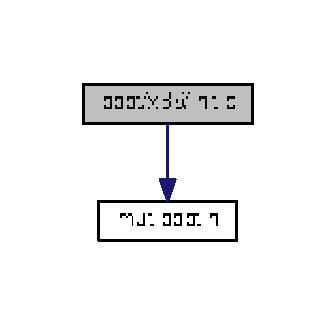
\includegraphics[width=161pt]{init_8c__incl}
\end{center}
\end{figure}
\subsection*{Classes}
\begin{DoxyCompactItemize}
\item 
struct \hyperlink{struct_f_i_r_m__sect}{F\+I\+R\+M\+\_\+sect}
\begin{DoxyCompactList}\small\item\em Contains one section of the F\+I\+R\+M format. \end{DoxyCompactList}\item 
struct \hyperlink{struct_f_i_r_m__header}{F\+I\+R\+M\+\_\+header}
\begin{DoxyCompactList}\small\item\em Contains the first sector of every F\+I\+R\+M file. \end{DoxyCompactList}\end{DoxyCompactItemize}
\subsection*{Functions}
\begin{DoxyCompactItemize}
\item 
struct \hyperlink{struct_f_i_r_m__sect}{F\+I\+R\+M\+\_\+sect} \hyperlink{init_8c_a10d79dd48dc82c172759244b582a9307}{\+\_\+\+\_\+attribute\+\_\+\+\_\+} ((packed))
\item 
void \hyperlink{init_8c_a1759742611d6bfa4566fa4a49eb720b2}{init} (int eax, struct \hyperlink{structmultiboot__info}{multiboot\+\_\+info} $\ast$mb\+\_\+info)
\begin{DoxyCompactList}\small\item\em This routine is called by boot.\+S This routine is called by boot.\+S. It loads and jumps to a F\+I\+R\+M binary. \end{DoxyCompactList}\end{DoxyCompactItemize}
\subsection*{Variables}
\begin{DoxyCompactItemize}
\item 
unsigned int \hyperlink{init_8c_a29b5297d3393519050e3126c4cb07c1c}{offset}
\item 
unsigned int \hyperlink{init_8c_a388bdfee4074b0bddcaabf1719bd4c58}{physical}
\begin{DoxyCompactList}\small\item\em Offset in file (bytes) \end{DoxyCompactList}\item 
unsigned int \hyperlink{init_8c_aac913b3a1f6ef005d66bf7a84428773e}{size}
\begin{DoxyCompactList}\small\item\em Physical address, where the section is copied to. \end{DoxyCompactList}\item 
unsigned int \hyperlink{init_8c_ae37ed54bd49226775904ceb6c6afb371}{arm11}
\begin{DoxyCompactList}\small\item\em Size of section. \end{DoxyCompactList}\item 
unsigned char \hyperlink{init_8c_a01b54fda0bed15306e272d0bfc9185d4}{S\+H\+A256} \mbox{[}0x20\mbox{]}
\begin{DoxyCompactList}\small\item\em currently unused \end{DoxyCompactList}\item 
char \hyperlink{init_8c_a03dedff415badb9581a8ca90e6a45b53}{magic} \mbox{[}4\mbox{]}
\item 
int \hyperlink{init_8c_aad880fc4455c253781e8968f2239d56f}{version}
\begin{DoxyCompactList}\small\item\em Magic \char`\"{}\+F\+I\+R\+M\char`\"{} string (not-\/null terminated) \end{DoxyCompactList}\item 
void($\ast$ \hyperlink{init_8c_ac77d736c7a6ce0e4cb1c6081311365fe}{entrypoint} )()
\begin{DoxyCompactList}\small\item\em Version. Currently 1. \end{DoxyCompactList}\item 
unsigned int \hyperlink{init_8c_ab8728043a657910cc02693dfd5cc5d7a}{reserved} \mbox{[}0x\+D\mbox{]}
\begin{DoxyCompactList}\small\item\em Address where the processor jumps to after loading. \end{DoxyCompactList}\item 
struct \hyperlink{struct_f_i_r_m__sect}{F\+I\+R\+M\+\_\+sect} \hyperlink{init_8c_a1e11470b0a65f8d9b7619857d1f19acf}{sections} \mbox{[}4\mbox{]}
\item 
unsigned char \hyperlink{init_8c_a374d9e480837445ab2ac3c57bd0d32d3}{R\+S\+A2048} \mbox{[}0x100\mbox{]}
\begin{DoxyCompactList}\small\item\em The four internal sections. \end{DoxyCompactList}\end{DoxyCompactItemize}


\subsection{Function Documentation}
\hypertarget{init_8c_a10d79dd48dc82c172759244b582a9307}{}\index{init.\+c@{init.\+c}!\+\_\+\+\_\+attribute\+\_\+\+\_\+@{\+\_\+\+\_\+attribute\+\_\+\+\_\+}}
\index{\+\_\+\+\_\+attribute\+\_\+\+\_\+@{\+\_\+\+\_\+attribute\+\_\+\+\_\+}!init.\+c@{init.\+c}}
\subsubsection[{\+\_\+\+\_\+attribute\+\_\+\+\_\+((packed))}]{\setlength{\rightskip}{0pt plus 5cm}struct {\bf F\+I\+R\+M\+\_\+sect} \+\_\+\+\_\+attribute\+\_\+\+\_\+ (
\begin{DoxyParamCaption}
\item[{(packed)}]{}
\end{DoxyParamCaption}
)}\label{init_8c_a10d79dd48dc82c172759244b582a9307}
\hypertarget{init_8c_a1759742611d6bfa4566fa4a49eb720b2}{}\index{init.\+c@{init.\+c}!init@{init}}
\index{init@{init}!init.\+c@{init.\+c}}
\subsubsection[{init(int eax, struct multiboot\+\_\+info $\ast$mb\+\_\+info)}]{\setlength{\rightskip}{0pt plus 5cm}init (
\begin{DoxyParamCaption}
\item[{int}]{eax, }
\item[{struct {\bf multiboot\+\_\+info} $\ast$}]{mb\+\_\+info}
\end{DoxyParamCaption}
)}\label{init_8c_a1759742611d6bfa4566fa4a49eb720b2}


This routine is called by boot.\+S This routine is called by boot.\+S. It loads and jumps to a F\+I\+R\+M binary. 



\subsection{Variable Documentation}
\hypertarget{init_8c_ae37ed54bd49226775904ceb6c6afb371}{}\index{init.\+c@{init.\+c}!arm11@{arm11}}
\index{arm11@{arm11}!init.\+c@{init.\+c}}
\subsubsection[{arm11}]{\setlength{\rightskip}{0pt plus 5cm}unsigned int arm11}\label{init_8c_ae37ed54bd49226775904ceb6c6afb371}


Size of section. 

\hypertarget{init_8c_ac77d736c7a6ce0e4cb1c6081311365fe}{}\index{init.\+c@{init.\+c}!entrypoint@{entrypoint}}
\index{entrypoint@{entrypoint}!init.\+c@{init.\+c}}
\subsubsection[{entrypoint}]{\setlength{\rightskip}{0pt plus 5cm}void($\ast$ entrypoint) ()}\label{init_8c_ac77d736c7a6ce0e4cb1c6081311365fe}


Version. Currently 1. 

\hypertarget{init_8c_a03dedff415badb9581a8ca90e6a45b53}{}\index{init.\+c@{init.\+c}!magic@{magic}}
\index{magic@{magic}!init.\+c@{init.\+c}}
\subsubsection[{magic}]{\setlength{\rightskip}{0pt plus 5cm}char magic\mbox{[}4\mbox{]}}\label{init_8c_a03dedff415badb9581a8ca90e6a45b53}
\hypertarget{init_8c_a29b5297d3393519050e3126c4cb07c1c}{}\index{init.\+c@{init.\+c}!offset@{offset}}
\index{offset@{offset}!init.\+c@{init.\+c}}
\subsubsection[{offset}]{\setlength{\rightskip}{0pt plus 5cm}unsigned int offset}\label{init_8c_a29b5297d3393519050e3126c4cb07c1c}
\hypertarget{init_8c_a388bdfee4074b0bddcaabf1719bd4c58}{}\index{init.\+c@{init.\+c}!physical@{physical}}
\index{physical@{physical}!init.\+c@{init.\+c}}
\subsubsection[{physical}]{\setlength{\rightskip}{0pt plus 5cm}unsigned int physical}\label{init_8c_a388bdfee4074b0bddcaabf1719bd4c58}


Offset in file (bytes) 

\hypertarget{init_8c_ab8728043a657910cc02693dfd5cc5d7a}{}\index{init.\+c@{init.\+c}!reserved@{reserved}}
\index{reserved@{reserved}!init.\+c@{init.\+c}}
\subsubsection[{reserved}]{\setlength{\rightskip}{0pt plus 5cm}unsigned int reserved\mbox{[}0x\+D\mbox{]}}\label{init_8c_ab8728043a657910cc02693dfd5cc5d7a}


Address where the processor jumps to after loading. 

\hypertarget{init_8c_a374d9e480837445ab2ac3c57bd0d32d3}{}\index{init.\+c@{init.\+c}!R\+S\+A2048@{R\+S\+A2048}}
\index{R\+S\+A2048@{R\+S\+A2048}!init.\+c@{init.\+c}}
\subsubsection[{R\+S\+A2048}]{\setlength{\rightskip}{0pt plus 5cm}unsigned char R\+S\+A2048\mbox{[}0x100\mbox{]}}\label{init_8c_a374d9e480837445ab2ac3c57bd0d32d3}


The four internal sections. 

\hypertarget{init_8c_a1e11470b0a65f8d9b7619857d1f19acf}{}\index{init.\+c@{init.\+c}!sections@{sections}}
\index{sections@{sections}!init.\+c@{init.\+c}}
\subsubsection[{sections}]{\setlength{\rightskip}{0pt plus 5cm}struct {\bf F\+I\+R\+M\+\_\+sect} sections\mbox{[}4\mbox{]}}\label{init_8c_a1e11470b0a65f8d9b7619857d1f19acf}
\hypertarget{init_8c_a01b54fda0bed15306e272d0bfc9185d4}{}\index{init.\+c@{init.\+c}!S\+H\+A256@{S\+H\+A256}}
\index{S\+H\+A256@{S\+H\+A256}!init.\+c@{init.\+c}}
\subsubsection[{S\+H\+A256}]{\setlength{\rightskip}{0pt plus 5cm}unsigned char S\+H\+A256\mbox{[}0x20\mbox{]}}\label{init_8c_a01b54fda0bed15306e272d0bfc9185d4}


currently unused 

\hypertarget{init_8c_aac913b3a1f6ef005d66bf7a84428773e}{}\index{init.\+c@{init.\+c}!size@{size}}
\index{size@{size}!init.\+c@{init.\+c}}
\subsubsection[{size}]{\setlength{\rightskip}{0pt plus 5cm}unsigned int size}\label{init_8c_aac913b3a1f6ef005d66bf7a84428773e}


Physical address, where the section is copied to. 

\hypertarget{init_8c_aad880fc4455c253781e8968f2239d56f}{}\index{init.\+c@{init.\+c}!version@{version}}
\index{version@{version}!init.\+c@{init.\+c}}
\subsubsection[{version}]{\setlength{\rightskip}{0pt plus 5cm}int version}\label{init_8c_aad880fc4455c253781e8968f2239d56f}


Magic \char`\"{}\+F\+I\+R\+M\char`\"{} string (not-\/null terminated) 


\hypertarget{multiboot_8h}{}\section{boot/x86/multiboot.h File Reference}
\label{multiboot_8h}\index{boot/x86/multiboot.\+h@{boot/x86/multiboot.\+h}}
This graph shows which files directly or indirectly include this file\+:\nopagebreak
\begin{figure}[H]
\begin{center}
\leavevmode
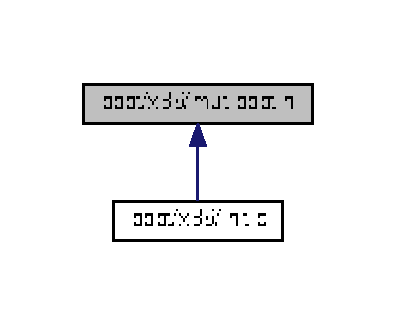
\includegraphics[width=190pt]{multiboot_8h__dep__incl}
\end{center}
\end{figure}
\subsection*{Classes}
\begin{DoxyCompactItemize}
\item 
struct \hyperlink{structmultiboot__header}{multiboot\+\_\+header}
\item 
struct \hyperlink{structmultiboot__aout__symbol__table}{multiboot\+\_\+aout\+\_\+symbol\+\_\+table}
\item 
struct \hyperlink{structmultiboot__elf__section__header__table}{multiboot\+\_\+elf\+\_\+section\+\_\+header\+\_\+table}
\item 
struct \hyperlink{structmultiboot__info}{multiboot\+\_\+info}
\item 
struct \hyperlink{structmultiboot__color}{multiboot\+\_\+color}
\item 
struct \hyperlink{structmultiboot__mmap__entry}{multiboot\+\_\+mmap\+\_\+entry}
\item 
struct \hyperlink{structmultiboot__mod__list}{multiboot\+\_\+mod\+\_\+list}
\item 
struct \hyperlink{structmultiboot__apm__info}{multiboot\+\_\+apm\+\_\+info}
\item 
struct \hyperlink{struct_m_o_d_e___i_n_f_o}{M\+O\+D\+E\+\_\+\+I\+N\+F\+O}
\end{DoxyCompactItemize}
\subsection*{Macros}
\begin{DoxyCompactItemize}
\item 
\#define \hyperlink{multiboot_8h_a0b53e2de91aa7498c4b476776b27e5f3}{M\+U\+L\+T\+I\+B\+O\+O\+T\+\_\+\+S\+E\+A\+R\+C\+H}~8192
\item 
\#define \hyperlink{multiboot_8h_abc554da6e5184d34e039b551177434ba}{M\+U\+L\+T\+I\+B\+O\+O\+T\+\_\+\+H\+E\+A\+D\+E\+R\+\_\+\+A\+L\+I\+G\+N}~4
\item 
\#define \hyperlink{multiboot_8h_ab36ad4b4a42c58aac4ad1f2ba13054e9}{M\+U\+L\+T\+I\+B\+O\+O\+T\+\_\+\+H\+E\+A\+D\+E\+R\+\_\+\+M\+A\+G\+I\+C}~0x1\+B\+A\+D\+B002
\item 
\#define \hyperlink{multiboot_8h_aacd617f4e3daafd6eab95fb6215ccae4}{M\+U\+L\+T\+I\+B\+O\+O\+T\+\_\+\+B\+O\+O\+T\+L\+O\+A\+D\+E\+R\+\_\+\+M\+A\+G\+I\+C}~0x2\+B\+A\+D\+B002
\item 
\#define \hyperlink{multiboot_8h_ab3284a28549f2a2f1a2001ca023aaa1e}{M\+U\+L\+T\+I\+B\+O\+O\+T\+\_\+\+M\+O\+D\+\_\+\+A\+L\+I\+G\+N}~0x00001000
\item 
\#define \hyperlink{multiboot_8h_a7f583196f43e30e93323f5e44554d726}{M\+U\+L\+T\+I\+B\+O\+O\+T\+\_\+\+I\+N\+F\+O\+\_\+\+A\+L\+I\+G\+N}~0x00000004
\item 
\#define \hyperlink{multiboot_8h_aab5e5487e858de2a031cd3f1232f7b60}{M\+U\+L\+T\+I\+B\+O\+O\+T\+\_\+\+P\+A\+G\+E\+\_\+\+A\+L\+I\+G\+N}~0x00000001
\item 
\#define \hyperlink{multiboot_8h_afdfca6bbbf4b7dca40e9d43e58201f55}{M\+U\+L\+T\+I\+B\+O\+O\+T\+\_\+\+M\+E\+M\+O\+R\+Y\+\_\+\+I\+N\+F\+O}~0x00000002
\item 
\#define \hyperlink{multiboot_8h_a74a1da9293ae3835241c60b2d9e65e8d}{M\+U\+L\+T\+I\+B\+O\+O\+T\+\_\+\+V\+I\+D\+E\+O\+\_\+\+M\+O\+D\+E}~0x00000004
\item 
\#define \hyperlink{multiboot_8h_a791f0c6a97c36de5388c990503ee4639}{M\+U\+L\+T\+I\+B\+O\+O\+T\+\_\+\+A\+O\+U\+T\+\_\+\+K\+L\+U\+D\+G\+E}~0x00010000
\item 
\#define \hyperlink{multiboot_8h_a1cb6047ede9a179b2958048573269d7a}{M\+U\+L\+T\+I\+B\+O\+O\+T\+\_\+\+I\+N\+F\+O\+\_\+\+M\+E\+M\+O\+R\+Y}~0x00000001
\item 
\#define \hyperlink{multiboot_8h_acfde5ffdd699c023dd8f4b89aa66556f}{M\+U\+L\+T\+I\+B\+O\+O\+T\+\_\+\+I\+N\+F\+O\+\_\+\+B\+O\+O\+T\+D\+E\+V}~0x00000002
\item 
\#define \hyperlink{multiboot_8h_ae75fb4f821b7ab405d46318d9b90a677}{M\+U\+L\+T\+I\+B\+O\+O\+T\+\_\+\+I\+N\+F\+O\+\_\+\+C\+M\+D\+L\+I\+N\+E}~0x00000004
\item 
\#define \hyperlink{multiboot_8h_a9a06a0175854cc6af54ddb6bd798c5bc}{M\+U\+L\+T\+I\+B\+O\+O\+T\+\_\+\+I\+N\+F\+O\+\_\+\+M\+O\+D\+S}~0x00000008
\item 
\#define \hyperlink{multiboot_8h_a186ab9e55c5bc612b9fd7e10b4be5600}{M\+U\+L\+T\+I\+B\+O\+O\+T\+\_\+\+I\+N\+F\+O\+\_\+\+A\+O\+U\+T\+\_\+\+S\+Y\+M\+S}~0x00000010
\item 
\#define \hyperlink{multiboot_8h_ad7d22ae99c11dc92152acdc8494a71f0}{M\+U\+L\+T\+I\+B\+O\+O\+T\+\_\+\+I\+N\+F\+O\+\_\+\+E\+L\+F\+\_\+\+S\+H\+D\+R}~0\+X00000020
\item 
\#define \hyperlink{multiboot_8h_a2d16dabdfdee01362c3457d06f0ff850}{M\+U\+L\+T\+I\+B\+O\+O\+T\+\_\+\+I\+N\+F\+O\+\_\+\+M\+E\+M\+\_\+\+M\+A\+P}~0x00000040
\item 
\#define \hyperlink{multiboot_8h_af2c5803d8cc6e1e8c00181ca546e68ab}{M\+U\+L\+T\+I\+B\+O\+O\+T\+\_\+\+I\+N\+F\+O\+\_\+\+D\+R\+I\+V\+E\+\_\+\+I\+N\+F\+O}~0x00000080
\item 
\#define \hyperlink{multiboot_8h_ad60e5b72325f5752e955879f3fbb44c3}{M\+U\+L\+T\+I\+B\+O\+O\+T\+\_\+\+I\+N\+F\+O\+\_\+\+C\+O\+N\+F\+I\+G\+\_\+\+T\+A\+B\+L\+E}~0x00000100
\item 
\#define \hyperlink{multiboot_8h_a9743476d5f32c9ae22f6254a0e3ba11d}{M\+U\+L\+T\+I\+B\+O\+O\+T\+\_\+\+I\+N\+F\+O\+\_\+\+B\+O\+O\+T\+\_\+\+L\+O\+A\+D\+E\+R\+\_\+\+N\+A\+M\+E}~0x00000200
\item 
\#define \hyperlink{multiboot_8h_aab73446f0cee2e9dc91f43eb9a0c806b}{M\+U\+L\+T\+I\+B\+O\+O\+T\+\_\+\+I\+N\+F\+O\+\_\+\+A\+P\+M\+\_\+\+T\+A\+B\+L\+E}~0x00000400
\item 
\#define \hyperlink{multiboot_8h_abf0a727e2e262407c77d54baf40d2f39}{M\+U\+L\+T\+I\+B\+O\+O\+T\+\_\+\+I\+N\+F\+O\+\_\+\+V\+B\+E\+\_\+\+I\+N\+F\+O}~0x00000800
\item 
\#define \hyperlink{multiboot_8h_a1c07b211ed2c374f5fbcf40c97bce2c0}{M\+U\+L\+T\+I\+B\+O\+O\+T\+\_\+\+I\+N\+F\+O\+\_\+\+F\+R\+A\+M\+E\+B\+U\+F\+F\+E\+R\+\_\+\+I\+N\+F\+O}~0x00001000
\item 
\#define \hyperlink{multiboot_8h_a8e2af641ff42074bb807c3ec9e33b2e0}{M\+U\+L\+T\+I\+B\+O\+O\+T\+\_\+\+F\+R\+A\+M\+E\+B\+U\+F\+F\+E\+R\+\_\+\+T\+Y\+P\+E\+\_\+\+I\+N\+D\+E\+X\+E\+D}~0
\item 
\#define \hyperlink{multiboot_8h_a34b2f01226ea42de22e06db7f652fbb1}{M\+U\+L\+T\+I\+B\+O\+O\+T\+\_\+\+F\+R\+A\+M\+E\+B\+U\+F\+F\+E\+R\+\_\+\+T\+Y\+P\+E\+\_\+\+R\+G\+B}~1
\item 
\#define \hyperlink{multiboot_8h_af6005f97267af2cb0ff37fb245284440}{M\+U\+L\+T\+I\+B\+O\+O\+T\+\_\+\+F\+R\+A\+M\+E\+B\+U\+F\+F\+E\+R\+\_\+\+T\+Y\+P\+E\+\_\+\+E\+G\+A\+\_\+\+T\+E\+X\+T}~2
\item 
\#define \hyperlink{multiboot_8h_a7fe141351ebcde0acbd6118ad0ea1a21}{M\+U\+L\+T\+I\+B\+O\+O\+T\+\_\+\+M\+E\+M\+O\+R\+Y\+\_\+\+A\+V\+A\+I\+L\+A\+B\+L\+E}~1
\item 
\#define \hyperlink{multiboot_8h_a0299aedc71e1f6707181471bafb18e7c}{M\+U\+L\+T\+I\+B\+O\+O\+T\+\_\+\+M\+E\+M\+O\+R\+Y\+\_\+\+R\+E\+S\+E\+R\+V\+E\+D}~2
\item 
\#define \hyperlink{multiboot_8h_af35be82586f332a561d00207c937ee57}{M\+U\+L\+T\+I\+B\+O\+O\+T\+\_\+\+M\+E\+M\+O\+R\+Y\+\_\+\+A\+C\+P\+I\+\_\+\+R\+E\+C\+L\+A\+I\+M\+A\+B\+L\+E}~3
\item 
\#define \hyperlink{multiboot_8h_a68f78286f7434d373a82f1b6f6473c72}{M\+U\+L\+T\+I\+B\+O\+O\+T\+\_\+\+M\+E\+M\+O\+R\+Y\+\_\+\+N\+V\+S}~4
\item 
\#define \hyperlink{multiboot_8h_a1604ec18ac949d88dab993904b08c075}{M\+U\+L\+T\+I\+B\+O\+O\+T\+\_\+\+M\+E\+M\+O\+R\+Y\+\_\+\+B\+A\+D\+R\+A\+M}~5
\end{DoxyCompactItemize}
\subsection*{Typedefs}
\begin{DoxyCompactItemize}
\item 
typedef unsigned char \hyperlink{multiboot_8h_a037f602538fccf97e90021c19fdfc047}{multiboot\+\_\+uint8\+\_\+t}
\item 
typedef unsigned short \hyperlink{multiboot_8h_a3a11e3c2b5e0617736a05343aa5795b3}{multiboot\+\_\+uint16\+\_\+t}
\item 
typedef unsigned int \hyperlink{multiboot_8h_a009f355da41fed4badb8a52d432f5186}{multiboot\+\_\+uint32\+\_\+t}
\item 
typedef unsigned long long \hyperlink{multiboot_8h_a8dfdd61648b48aa31845db590970e06a}{multiboot\+\_\+uint64\+\_\+t}
\item 
typedef struct \hyperlink{structmultiboot__aout__symbol__table}{multiboot\+\_\+aout\+\_\+symbol\+\_\+table} \hyperlink{multiboot_8h_a2f11acfde9ee0022a999f69d3e972352}{multiboot\+\_\+aout\+\_\+symbol\+\_\+table\+\_\+t}
\item 
typedef struct \hyperlink{structmultiboot__elf__section__header__table}{multiboot\+\_\+elf\+\_\+section\+\_\+header\+\_\+table} \hyperlink{multiboot_8h_a2ea4dd45da23724e95b9fc701b41d1e0}{multiboot\+\_\+elf\+\_\+section\+\_\+header\+\_\+table\+\_\+t}
\item 
typedef struct \hyperlink{structmultiboot__info}{multiboot\+\_\+info} \hyperlink{multiboot_8h_a8cb99862e8314c32c007eee9d2481ae1}{multiboot\+\_\+info\+\_\+t}
\item 
typedef struct \hyperlink{structmultiboot__mmap__entry}{multiboot\+\_\+mmap\+\_\+entry} \hyperlink{multiboot_8h_a2aa16c58ceb6b9548aded205e46e8a3b}{multiboot\+\_\+memory\+\_\+map\+\_\+t}
\item 
typedef struct \hyperlink{structmultiboot__mod__list}{multiboot\+\_\+mod\+\_\+list} \hyperlink{multiboot_8h_a84f7545f2c7b26164fed10a81bd052fd}{multiboot\+\_\+module\+\_\+t}
\end{DoxyCompactItemize}
\subsection*{Functions}
\begin{DoxyCompactItemize}
\item 
struct \hyperlink{structmultiboot__mmap__entry}{multiboot\+\_\+mmap\+\_\+entry} \hyperlink{multiboot_8h_aa6b9a7218d544abc2be2bd335681b0a1}{\+\_\+\+\_\+attribute\+\_\+\+\_\+} ((packed))
\end{DoxyCompactItemize}
\subsection*{Variables}
\begin{DoxyCompactItemize}
\item 
struct \hyperlink{structmultiboot__header}{multiboot\+\_\+header} \hyperlink{multiboot_8h_a76ae64e1ba3c94e0e9259d974f69e347}{\+\_\+\+\_\+attribute\+\_\+\+\_\+}
\item 
\hyperlink{multiboot_8h_a009f355da41fed4badb8a52d432f5186}{multiboot\+\_\+uint32\+\_\+t} \hyperlink{multiboot_8h_a6d813a0f2b5281b18dea3f4cda696c33}{size}
\item 
\hyperlink{multiboot_8h_a8dfdd61648b48aa31845db590970e06a}{multiboot\+\_\+uint64\+\_\+t} \hyperlink{multiboot_8h_a8286ae6db03c34c4bb161accbfbfbbcd}{addr}
\item 
\hyperlink{multiboot_8h_a8dfdd61648b48aa31845db590970e06a}{multiboot\+\_\+uint64\+\_\+t} \hyperlink{multiboot_8h_a6de3a6d27a7e07942958b912d39792e6}{len}
\item 
\hyperlink{multiboot_8h_a009f355da41fed4badb8a52d432f5186}{multiboot\+\_\+uint32\+\_\+t} \hyperlink{multiboot_8h_a8da1a8c7127a0371eec0810a29e30f3c}{type}
\item 
unsigned short \hyperlink{multiboot_8h_a2a883485beac6e6bb89b8a312cba3eaa}{Mode\+Attributes}
\item 
unsigned char \hyperlink{multiboot_8h_a473b734c6c5bb31318d8c324033c6137}{Win\+A\+Attributes}
\item 
unsigned char \hyperlink{multiboot_8h_ab6b6baadbf99c7d22dc5b356c11b1024}{Win\+B\+Attributes}
\item 
unsigned short \hyperlink{multiboot_8h_a1314919d3adc5ce476485a0b661caa35}{Win\+Granularity}
\item 
unsigned short \hyperlink{multiboot_8h_ad941e7fba5d18f68c2df5fda788ea3dc}{Win\+Size}
\item 
unsigned short \hyperlink{multiboot_8h_ad8d1f6d8b819324676126703a83aded8}{Win\+A\+Segment}
\item 
unsigned short \hyperlink{multiboot_8h_a93f7e14734b066b3a4bd03735c731f0e}{Win\+B\+Segment}
\item 
unsigned int \hyperlink{multiboot_8h_aa8e5e344747e1728272844be5104c093}{Win\+Func\+Ptr}
\item 
unsigned short \hyperlink{multiboot_8h_a99eea0fc9de5852642efca8a25b4d753}{Bytes\+Per\+Scan\+Line}
\item 
unsigned short \hyperlink{multiboot_8h_a5bf23b66f6450da4b07ddc59eff724da}{X\+Resolution}
\item 
unsigned short \hyperlink{multiboot_8h_a7b476e7dcc02468d587ebca1d20b85a1}{Y\+Resolution}
\item 
unsigned char \hyperlink{multiboot_8h_ae4ec2504a1c1304a504858abbedf00f1}{X\+Char\+Size}
\item 
unsigned char \hyperlink{multiboot_8h_a1508179761ab4c4af6edf0befb48a6bf}{Y\+Char\+Size}
\item 
unsigned char \hyperlink{multiboot_8h_aa1b05acb09bf7197679f5ae3f954bcd6}{Number\+Of\+Planes}
\item 
unsigned char \hyperlink{multiboot_8h_a27849358fc386f9e3a8314fc69883ece}{Bits\+Per\+Pixel}
\item 
unsigned char \hyperlink{multiboot_8h_a2859b02f75b5563fab60d1e88c805e50}{Number\+Of\+Banks}
\item 
unsigned char \hyperlink{multiboot_8h_a7049e1fe402c1ba8e2d19da1bb9ea237}{Memory\+Model}
\item 
unsigned char \hyperlink{multiboot_8h_a696508b5c8c166e97d4f597c720d4067}{Bank\+Size}
\item 
unsigned char \hyperlink{multiboot_8h_a1aae79b073555a7651874a3337c708c9}{Number\+Of\+Image\+Pages}
\item 
unsigned char \hyperlink{multiboot_8h_a471b5031c20fa684175b99daf343ddbf}{Reserved\+\_\+page}
\item 
unsigned char \hyperlink{multiboot_8h_ab075edb62d8c493b0db868fbaa704b9e}{Red\+Mask\+Size}
\item 
unsigned char \hyperlink{multiboot_8h_afc688bb02ec93b5f4238832fbb75bef1}{Red\+Mask\+Pos}
\item 
unsigned char \hyperlink{multiboot_8h_a4fbf297ec44224778127b7321ec216ac}{Green\+Mask\+Size}
\item 
unsigned char \hyperlink{multiboot_8h_a4a6db3c822dad9fe2611e90adf6a1b45}{Green\+Mask\+Pos}
\item 
unsigned char \hyperlink{multiboot_8h_a0a1b16f85b9b13785a96d3f9b7c203f2}{Blue\+Mask\+Size}
\item 
unsigned char \hyperlink{multiboot_8h_a612cd0d43e45e8391a9881f48f8a40ea}{Blue\+Mask\+Pos}
\item 
unsigned char \hyperlink{multiboot_8h_a13f5f8c137757a8e11697cf914f68f3f}{Reserved\+Mask\+Size}
\item 
unsigned char \hyperlink{multiboot_8h_a7e024175e59a1ce58adf517959c92e00}{Reserved\+Mask\+Pos}
\item 
unsigned char \hyperlink{multiboot_8h_ab59c32426fe5932cddde6f966f4f3d30}{Direct\+Color\+Mode\+Info}
\item 
unsigned int \hyperlink{multiboot_8h_a77de1ce0d09cf610c31a1301f7cd5520}{Phys\+Base\+Ptr}
\item 
unsigned int \hyperlink{multiboot_8h_a38efd8108381f08d44b42ce851fedc0b}{Off\+Screen\+Mem\+Offset}
\item 
unsigned short \hyperlink{multiboot_8h_ab4ff4006b01440fca4185213a59d8a6e}{Off\+Screen\+Mem\+Size}
\item 
unsigned char \hyperlink{multiboot_8h_ae7b52b0eae5b6a50092bdb2535e6833e}{Reserved} \mbox{[}206\mbox{]}
\end{DoxyCompactItemize}


\subsection{Macro Definition Documentation}
\hypertarget{multiboot_8h_a791f0c6a97c36de5388c990503ee4639}{}\index{multiboot.\+h@{multiboot.\+h}!M\+U\+L\+T\+I\+B\+O\+O\+T\+\_\+\+A\+O\+U\+T\+\_\+\+K\+L\+U\+D\+G\+E@{M\+U\+L\+T\+I\+B\+O\+O\+T\+\_\+\+A\+O\+U\+T\+\_\+\+K\+L\+U\+D\+G\+E}}
\index{M\+U\+L\+T\+I\+B\+O\+O\+T\+\_\+\+A\+O\+U\+T\+\_\+\+K\+L\+U\+D\+G\+E@{M\+U\+L\+T\+I\+B\+O\+O\+T\+\_\+\+A\+O\+U\+T\+\_\+\+K\+L\+U\+D\+G\+E}!multiboot.\+h@{multiboot.\+h}}
\subsubsection[{M\+U\+L\+T\+I\+B\+O\+O\+T\+\_\+\+A\+O\+U\+T\+\_\+\+K\+L\+U\+D\+G\+E}]{\setlength{\rightskip}{0pt plus 5cm}\#define M\+U\+L\+T\+I\+B\+O\+O\+T\+\_\+\+A\+O\+U\+T\+\_\+\+K\+L\+U\+D\+G\+E~0x00010000}\label{multiboot_8h_a791f0c6a97c36de5388c990503ee4639}
\hypertarget{multiboot_8h_aacd617f4e3daafd6eab95fb6215ccae4}{}\index{multiboot.\+h@{multiboot.\+h}!M\+U\+L\+T\+I\+B\+O\+O\+T\+\_\+\+B\+O\+O\+T\+L\+O\+A\+D\+E\+R\+\_\+\+M\+A\+G\+I\+C@{M\+U\+L\+T\+I\+B\+O\+O\+T\+\_\+\+B\+O\+O\+T\+L\+O\+A\+D\+E\+R\+\_\+\+M\+A\+G\+I\+C}}
\index{M\+U\+L\+T\+I\+B\+O\+O\+T\+\_\+\+B\+O\+O\+T\+L\+O\+A\+D\+E\+R\+\_\+\+M\+A\+G\+I\+C@{M\+U\+L\+T\+I\+B\+O\+O\+T\+\_\+\+B\+O\+O\+T\+L\+O\+A\+D\+E\+R\+\_\+\+M\+A\+G\+I\+C}!multiboot.\+h@{multiboot.\+h}}
\subsubsection[{M\+U\+L\+T\+I\+B\+O\+O\+T\+\_\+\+B\+O\+O\+T\+L\+O\+A\+D\+E\+R\+\_\+\+M\+A\+G\+I\+C}]{\setlength{\rightskip}{0pt plus 5cm}\#define M\+U\+L\+T\+I\+B\+O\+O\+T\+\_\+\+B\+O\+O\+T\+L\+O\+A\+D\+E\+R\+\_\+\+M\+A\+G\+I\+C~0x2\+B\+A\+D\+B002}\label{multiboot_8h_aacd617f4e3daafd6eab95fb6215ccae4}
\hypertarget{multiboot_8h_af6005f97267af2cb0ff37fb245284440}{}\index{multiboot.\+h@{multiboot.\+h}!M\+U\+L\+T\+I\+B\+O\+O\+T\+\_\+\+F\+R\+A\+M\+E\+B\+U\+F\+F\+E\+R\+\_\+\+T\+Y\+P\+E\+\_\+\+E\+G\+A\+\_\+\+T\+E\+X\+T@{M\+U\+L\+T\+I\+B\+O\+O\+T\+\_\+\+F\+R\+A\+M\+E\+B\+U\+F\+F\+E\+R\+\_\+\+T\+Y\+P\+E\+\_\+\+E\+G\+A\+\_\+\+T\+E\+X\+T}}
\index{M\+U\+L\+T\+I\+B\+O\+O\+T\+\_\+\+F\+R\+A\+M\+E\+B\+U\+F\+F\+E\+R\+\_\+\+T\+Y\+P\+E\+\_\+\+E\+G\+A\+\_\+\+T\+E\+X\+T@{M\+U\+L\+T\+I\+B\+O\+O\+T\+\_\+\+F\+R\+A\+M\+E\+B\+U\+F\+F\+E\+R\+\_\+\+T\+Y\+P\+E\+\_\+\+E\+G\+A\+\_\+\+T\+E\+X\+T}!multiboot.\+h@{multiboot.\+h}}
\subsubsection[{M\+U\+L\+T\+I\+B\+O\+O\+T\+\_\+\+F\+R\+A\+M\+E\+B\+U\+F\+F\+E\+R\+\_\+\+T\+Y\+P\+E\+\_\+\+E\+G\+A\+\_\+\+T\+E\+X\+T}]{\setlength{\rightskip}{0pt plus 5cm}\#define M\+U\+L\+T\+I\+B\+O\+O\+T\+\_\+\+F\+R\+A\+M\+E\+B\+U\+F\+F\+E\+R\+\_\+\+T\+Y\+P\+E\+\_\+\+E\+G\+A\+\_\+\+T\+E\+X\+T~2}\label{multiboot_8h_af6005f97267af2cb0ff37fb245284440}
\hypertarget{multiboot_8h_a8e2af641ff42074bb807c3ec9e33b2e0}{}\index{multiboot.\+h@{multiboot.\+h}!M\+U\+L\+T\+I\+B\+O\+O\+T\+\_\+\+F\+R\+A\+M\+E\+B\+U\+F\+F\+E\+R\+\_\+\+T\+Y\+P\+E\+\_\+\+I\+N\+D\+E\+X\+E\+D@{M\+U\+L\+T\+I\+B\+O\+O\+T\+\_\+\+F\+R\+A\+M\+E\+B\+U\+F\+F\+E\+R\+\_\+\+T\+Y\+P\+E\+\_\+\+I\+N\+D\+E\+X\+E\+D}}
\index{M\+U\+L\+T\+I\+B\+O\+O\+T\+\_\+\+F\+R\+A\+M\+E\+B\+U\+F\+F\+E\+R\+\_\+\+T\+Y\+P\+E\+\_\+\+I\+N\+D\+E\+X\+E\+D@{M\+U\+L\+T\+I\+B\+O\+O\+T\+\_\+\+F\+R\+A\+M\+E\+B\+U\+F\+F\+E\+R\+\_\+\+T\+Y\+P\+E\+\_\+\+I\+N\+D\+E\+X\+E\+D}!multiboot.\+h@{multiboot.\+h}}
\subsubsection[{M\+U\+L\+T\+I\+B\+O\+O\+T\+\_\+\+F\+R\+A\+M\+E\+B\+U\+F\+F\+E\+R\+\_\+\+T\+Y\+P\+E\+\_\+\+I\+N\+D\+E\+X\+E\+D}]{\setlength{\rightskip}{0pt plus 5cm}\#define M\+U\+L\+T\+I\+B\+O\+O\+T\+\_\+\+F\+R\+A\+M\+E\+B\+U\+F\+F\+E\+R\+\_\+\+T\+Y\+P\+E\+\_\+\+I\+N\+D\+E\+X\+E\+D~0}\label{multiboot_8h_a8e2af641ff42074bb807c3ec9e33b2e0}
\hypertarget{multiboot_8h_a34b2f01226ea42de22e06db7f652fbb1}{}\index{multiboot.\+h@{multiboot.\+h}!M\+U\+L\+T\+I\+B\+O\+O\+T\+\_\+\+F\+R\+A\+M\+E\+B\+U\+F\+F\+E\+R\+\_\+\+T\+Y\+P\+E\+\_\+\+R\+G\+B@{M\+U\+L\+T\+I\+B\+O\+O\+T\+\_\+\+F\+R\+A\+M\+E\+B\+U\+F\+F\+E\+R\+\_\+\+T\+Y\+P\+E\+\_\+\+R\+G\+B}}
\index{M\+U\+L\+T\+I\+B\+O\+O\+T\+\_\+\+F\+R\+A\+M\+E\+B\+U\+F\+F\+E\+R\+\_\+\+T\+Y\+P\+E\+\_\+\+R\+G\+B@{M\+U\+L\+T\+I\+B\+O\+O\+T\+\_\+\+F\+R\+A\+M\+E\+B\+U\+F\+F\+E\+R\+\_\+\+T\+Y\+P\+E\+\_\+\+R\+G\+B}!multiboot.\+h@{multiboot.\+h}}
\subsubsection[{M\+U\+L\+T\+I\+B\+O\+O\+T\+\_\+\+F\+R\+A\+M\+E\+B\+U\+F\+F\+E\+R\+\_\+\+T\+Y\+P\+E\+\_\+\+R\+G\+B}]{\setlength{\rightskip}{0pt plus 5cm}\#define M\+U\+L\+T\+I\+B\+O\+O\+T\+\_\+\+F\+R\+A\+M\+E\+B\+U\+F\+F\+E\+R\+\_\+\+T\+Y\+P\+E\+\_\+\+R\+G\+B~1}\label{multiboot_8h_a34b2f01226ea42de22e06db7f652fbb1}
\hypertarget{multiboot_8h_abc554da6e5184d34e039b551177434ba}{}\index{multiboot.\+h@{multiboot.\+h}!M\+U\+L\+T\+I\+B\+O\+O\+T\+\_\+\+H\+E\+A\+D\+E\+R\+\_\+\+A\+L\+I\+G\+N@{M\+U\+L\+T\+I\+B\+O\+O\+T\+\_\+\+H\+E\+A\+D\+E\+R\+\_\+\+A\+L\+I\+G\+N}}
\index{M\+U\+L\+T\+I\+B\+O\+O\+T\+\_\+\+H\+E\+A\+D\+E\+R\+\_\+\+A\+L\+I\+G\+N@{M\+U\+L\+T\+I\+B\+O\+O\+T\+\_\+\+H\+E\+A\+D\+E\+R\+\_\+\+A\+L\+I\+G\+N}!multiboot.\+h@{multiboot.\+h}}
\subsubsection[{M\+U\+L\+T\+I\+B\+O\+O\+T\+\_\+\+H\+E\+A\+D\+E\+R\+\_\+\+A\+L\+I\+G\+N}]{\setlength{\rightskip}{0pt plus 5cm}\#define M\+U\+L\+T\+I\+B\+O\+O\+T\+\_\+\+H\+E\+A\+D\+E\+R\+\_\+\+A\+L\+I\+G\+N~4}\label{multiboot_8h_abc554da6e5184d34e039b551177434ba}
\hypertarget{multiboot_8h_ab36ad4b4a42c58aac4ad1f2ba13054e9}{}\index{multiboot.\+h@{multiboot.\+h}!M\+U\+L\+T\+I\+B\+O\+O\+T\+\_\+\+H\+E\+A\+D\+E\+R\+\_\+\+M\+A\+G\+I\+C@{M\+U\+L\+T\+I\+B\+O\+O\+T\+\_\+\+H\+E\+A\+D\+E\+R\+\_\+\+M\+A\+G\+I\+C}}
\index{M\+U\+L\+T\+I\+B\+O\+O\+T\+\_\+\+H\+E\+A\+D\+E\+R\+\_\+\+M\+A\+G\+I\+C@{M\+U\+L\+T\+I\+B\+O\+O\+T\+\_\+\+H\+E\+A\+D\+E\+R\+\_\+\+M\+A\+G\+I\+C}!multiboot.\+h@{multiboot.\+h}}
\subsubsection[{M\+U\+L\+T\+I\+B\+O\+O\+T\+\_\+\+H\+E\+A\+D\+E\+R\+\_\+\+M\+A\+G\+I\+C}]{\setlength{\rightskip}{0pt plus 5cm}\#define M\+U\+L\+T\+I\+B\+O\+O\+T\+\_\+\+H\+E\+A\+D\+E\+R\+\_\+\+M\+A\+G\+I\+C~0x1\+B\+A\+D\+B002}\label{multiboot_8h_ab36ad4b4a42c58aac4ad1f2ba13054e9}
\hypertarget{multiboot_8h_a7f583196f43e30e93323f5e44554d726}{}\index{multiboot.\+h@{multiboot.\+h}!M\+U\+L\+T\+I\+B\+O\+O\+T\+\_\+\+I\+N\+F\+O\+\_\+\+A\+L\+I\+G\+N@{M\+U\+L\+T\+I\+B\+O\+O\+T\+\_\+\+I\+N\+F\+O\+\_\+\+A\+L\+I\+G\+N}}
\index{M\+U\+L\+T\+I\+B\+O\+O\+T\+\_\+\+I\+N\+F\+O\+\_\+\+A\+L\+I\+G\+N@{M\+U\+L\+T\+I\+B\+O\+O\+T\+\_\+\+I\+N\+F\+O\+\_\+\+A\+L\+I\+G\+N}!multiboot.\+h@{multiboot.\+h}}
\subsubsection[{M\+U\+L\+T\+I\+B\+O\+O\+T\+\_\+\+I\+N\+F\+O\+\_\+\+A\+L\+I\+G\+N}]{\setlength{\rightskip}{0pt plus 5cm}\#define M\+U\+L\+T\+I\+B\+O\+O\+T\+\_\+\+I\+N\+F\+O\+\_\+\+A\+L\+I\+G\+N~0x00000004}\label{multiboot_8h_a7f583196f43e30e93323f5e44554d726}
\hypertarget{multiboot_8h_a186ab9e55c5bc612b9fd7e10b4be5600}{}\index{multiboot.\+h@{multiboot.\+h}!M\+U\+L\+T\+I\+B\+O\+O\+T\+\_\+\+I\+N\+F\+O\+\_\+\+A\+O\+U\+T\+\_\+\+S\+Y\+M\+S@{M\+U\+L\+T\+I\+B\+O\+O\+T\+\_\+\+I\+N\+F\+O\+\_\+\+A\+O\+U\+T\+\_\+\+S\+Y\+M\+S}}
\index{M\+U\+L\+T\+I\+B\+O\+O\+T\+\_\+\+I\+N\+F\+O\+\_\+\+A\+O\+U\+T\+\_\+\+S\+Y\+M\+S@{M\+U\+L\+T\+I\+B\+O\+O\+T\+\_\+\+I\+N\+F\+O\+\_\+\+A\+O\+U\+T\+\_\+\+S\+Y\+M\+S}!multiboot.\+h@{multiboot.\+h}}
\subsubsection[{M\+U\+L\+T\+I\+B\+O\+O\+T\+\_\+\+I\+N\+F\+O\+\_\+\+A\+O\+U\+T\+\_\+\+S\+Y\+M\+S}]{\setlength{\rightskip}{0pt plus 5cm}\#define M\+U\+L\+T\+I\+B\+O\+O\+T\+\_\+\+I\+N\+F\+O\+\_\+\+A\+O\+U\+T\+\_\+\+S\+Y\+M\+S~0x00000010}\label{multiboot_8h_a186ab9e55c5bc612b9fd7e10b4be5600}
\hypertarget{multiboot_8h_aab73446f0cee2e9dc91f43eb9a0c806b}{}\index{multiboot.\+h@{multiboot.\+h}!M\+U\+L\+T\+I\+B\+O\+O\+T\+\_\+\+I\+N\+F\+O\+\_\+\+A\+P\+M\+\_\+\+T\+A\+B\+L\+E@{M\+U\+L\+T\+I\+B\+O\+O\+T\+\_\+\+I\+N\+F\+O\+\_\+\+A\+P\+M\+\_\+\+T\+A\+B\+L\+E}}
\index{M\+U\+L\+T\+I\+B\+O\+O\+T\+\_\+\+I\+N\+F\+O\+\_\+\+A\+P\+M\+\_\+\+T\+A\+B\+L\+E@{M\+U\+L\+T\+I\+B\+O\+O\+T\+\_\+\+I\+N\+F\+O\+\_\+\+A\+P\+M\+\_\+\+T\+A\+B\+L\+E}!multiboot.\+h@{multiboot.\+h}}
\subsubsection[{M\+U\+L\+T\+I\+B\+O\+O\+T\+\_\+\+I\+N\+F\+O\+\_\+\+A\+P\+M\+\_\+\+T\+A\+B\+L\+E}]{\setlength{\rightskip}{0pt plus 5cm}\#define M\+U\+L\+T\+I\+B\+O\+O\+T\+\_\+\+I\+N\+F\+O\+\_\+\+A\+P\+M\+\_\+\+T\+A\+B\+L\+E~0x00000400}\label{multiboot_8h_aab73446f0cee2e9dc91f43eb9a0c806b}
\hypertarget{multiboot_8h_a9743476d5f32c9ae22f6254a0e3ba11d}{}\index{multiboot.\+h@{multiboot.\+h}!M\+U\+L\+T\+I\+B\+O\+O\+T\+\_\+\+I\+N\+F\+O\+\_\+\+B\+O\+O\+T\+\_\+\+L\+O\+A\+D\+E\+R\+\_\+\+N\+A\+M\+E@{M\+U\+L\+T\+I\+B\+O\+O\+T\+\_\+\+I\+N\+F\+O\+\_\+\+B\+O\+O\+T\+\_\+\+L\+O\+A\+D\+E\+R\+\_\+\+N\+A\+M\+E}}
\index{M\+U\+L\+T\+I\+B\+O\+O\+T\+\_\+\+I\+N\+F\+O\+\_\+\+B\+O\+O\+T\+\_\+\+L\+O\+A\+D\+E\+R\+\_\+\+N\+A\+M\+E@{M\+U\+L\+T\+I\+B\+O\+O\+T\+\_\+\+I\+N\+F\+O\+\_\+\+B\+O\+O\+T\+\_\+\+L\+O\+A\+D\+E\+R\+\_\+\+N\+A\+M\+E}!multiboot.\+h@{multiboot.\+h}}
\subsubsection[{M\+U\+L\+T\+I\+B\+O\+O\+T\+\_\+\+I\+N\+F\+O\+\_\+\+B\+O\+O\+T\+\_\+\+L\+O\+A\+D\+E\+R\+\_\+\+N\+A\+M\+E}]{\setlength{\rightskip}{0pt plus 5cm}\#define M\+U\+L\+T\+I\+B\+O\+O\+T\+\_\+\+I\+N\+F\+O\+\_\+\+B\+O\+O\+T\+\_\+\+L\+O\+A\+D\+E\+R\+\_\+\+N\+A\+M\+E~0x00000200}\label{multiboot_8h_a9743476d5f32c9ae22f6254a0e3ba11d}
\hypertarget{multiboot_8h_acfde5ffdd699c023dd8f4b89aa66556f}{}\index{multiboot.\+h@{multiboot.\+h}!M\+U\+L\+T\+I\+B\+O\+O\+T\+\_\+\+I\+N\+F\+O\+\_\+\+B\+O\+O\+T\+D\+E\+V@{M\+U\+L\+T\+I\+B\+O\+O\+T\+\_\+\+I\+N\+F\+O\+\_\+\+B\+O\+O\+T\+D\+E\+V}}
\index{M\+U\+L\+T\+I\+B\+O\+O\+T\+\_\+\+I\+N\+F\+O\+\_\+\+B\+O\+O\+T\+D\+E\+V@{M\+U\+L\+T\+I\+B\+O\+O\+T\+\_\+\+I\+N\+F\+O\+\_\+\+B\+O\+O\+T\+D\+E\+V}!multiboot.\+h@{multiboot.\+h}}
\subsubsection[{M\+U\+L\+T\+I\+B\+O\+O\+T\+\_\+\+I\+N\+F\+O\+\_\+\+B\+O\+O\+T\+D\+E\+V}]{\setlength{\rightskip}{0pt plus 5cm}\#define M\+U\+L\+T\+I\+B\+O\+O\+T\+\_\+\+I\+N\+F\+O\+\_\+\+B\+O\+O\+T\+D\+E\+V~0x00000002}\label{multiboot_8h_acfde5ffdd699c023dd8f4b89aa66556f}
\hypertarget{multiboot_8h_ae75fb4f821b7ab405d46318d9b90a677}{}\index{multiboot.\+h@{multiboot.\+h}!M\+U\+L\+T\+I\+B\+O\+O\+T\+\_\+\+I\+N\+F\+O\+\_\+\+C\+M\+D\+L\+I\+N\+E@{M\+U\+L\+T\+I\+B\+O\+O\+T\+\_\+\+I\+N\+F\+O\+\_\+\+C\+M\+D\+L\+I\+N\+E}}
\index{M\+U\+L\+T\+I\+B\+O\+O\+T\+\_\+\+I\+N\+F\+O\+\_\+\+C\+M\+D\+L\+I\+N\+E@{M\+U\+L\+T\+I\+B\+O\+O\+T\+\_\+\+I\+N\+F\+O\+\_\+\+C\+M\+D\+L\+I\+N\+E}!multiboot.\+h@{multiboot.\+h}}
\subsubsection[{M\+U\+L\+T\+I\+B\+O\+O\+T\+\_\+\+I\+N\+F\+O\+\_\+\+C\+M\+D\+L\+I\+N\+E}]{\setlength{\rightskip}{0pt plus 5cm}\#define M\+U\+L\+T\+I\+B\+O\+O\+T\+\_\+\+I\+N\+F\+O\+\_\+\+C\+M\+D\+L\+I\+N\+E~0x00000004}\label{multiboot_8h_ae75fb4f821b7ab405d46318d9b90a677}
\hypertarget{multiboot_8h_ad60e5b72325f5752e955879f3fbb44c3}{}\index{multiboot.\+h@{multiboot.\+h}!M\+U\+L\+T\+I\+B\+O\+O\+T\+\_\+\+I\+N\+F\+O\+\_\+\+C\+O\+N\+F\+I\+G\+\_\+\+T\+A\+B\+L\+E@{M\+U\+L\+T\+I\+B\+O\+O\+T\+\_\+\+I\+N\+F\+O\+\_\+\+C\+O\+N\+F\+I\+G\+\_\+\+T\+A\+B\+L\+E}}
\index{M\+U\+L\+T\+I\+B\+O\+O\+T\+\_\+\+I\+N\+F\+O\+\_\+\+C\+O\+N\+F\+I\+G\+\_\+\+T\+A\+B\+L\+E@{M\+U\+L\+T\+I\+B\+O\+O\+T\+\_\+\+I\+N\+F\+O\+\_\+\+C\+O\+N\+F\+I\+G\+\_\+\+T\+A\+B\+L\+E}!multiboot.\+h@{multiboot.\+h}}
\subsubsection[{M\+U\+L\+T\+I\+B\+O\+O\+T\+\_\+\+I\+N\+F\+O\+\_\+\+C\+O\+N\+F\+I\+G\+\_\+\+T\+A\+B\+L\+E}]{\setlength{\rightskip}{0pt plus 5cm}\#define M\+U\+L\+T\+I\+B\+O\+O\+T\+\_\+\+I\+N\+F\+O\+\_\+\+C\+O\+N\+F\+I\+G\+\_\+\+T\+A\+B\+L\+E~0x00000100}\label{multiboot_8h_ad60e5b72325f5752e955879f3fbb44c3}
\hypertarget{multiboot_8h_af2c5803d8cc6e1e8c00181ca546e68ab}{}\index{multiboot.\+h@{multiboot.\+h}!M\+U\+L\+T\+I\+B\+O\+O\+T\+\_\+\+I\+N\+F\+O\+\_\+\+D\+R\+I\+V\+E\+\_\+\+I\+N\+F\+O@{M\+U\+L\+T\+I\+B\+O\+O\+T\+\_\+\+I\+N\+F\+O\+\_\+\+D\+R\+I\+V\+E\+\_\+\+I\+N\+F\+O}}
\index{M\+U\+L\+T\+I\+B\+O\+O\+T\+\_\+\+I\+N\+F\+O\+\_\+\+D\+R\+I\+V\+E\+\_\+\+I\+N\+F\+O@{M\+U\+L\+T\+I\+B\+O\+O\+T\+\_\+\+I\+N\+F\+O\+\_\+\+D\+R\+I\+V\+E\+\_\+\+I\+N\+F\+O}!multiboot.\+h@{multiboot.\+h}}
\subsubsection[{M\+U\+L\+T\+I\+B\+O\+O\+T\+\_\+\+I\+N\+F\+O\+\_\+\+D\+R\+I\+V\+E\+\_\+\+I\+N\+F\+O}]{\setlength{\rightskip}{0pt plus 5cm}\#define M\+U\+L\+T\+I\+B\+O\+O\+T\+\_\+\+I\+N\+F\+O\+\_\+\+D\+R\+I\+V\+E\+\_\+\+I\+N\+F\+O~0x00000080}\label{multiboot_8h_af2c5803d8cc6e1e8c00181ca546e68ab}
\hypertarget{multiboot_8h_ad7d22ae99c11dc92152acdc8494a71f0}{}\index{multiboot.\+h@{multiboot.\+h}!M\+U\+L\+T\+I\+B\+O\+O\+T\+\_\+\+I\+N\+F\+O\+\_\+\+E\+L\+F\+\_\+\+S\+H\+D\+R@{M\+U\+L\+T\+I\+B\+O\+O\+T\+\_\+\+I\+N\+F\+O\+\_\+\+E\+L\+F\+\_\+\+S\+H\+D\+R}}
\index{M\+U\+L\+T\+I\+B\+O\+O\+T\+\_\+\+I\+N\+F\+O\+\_\+\+E\+L\+F\+\_\+\+S\+H\+D\+R@{M\+U\+L\+T\+I\+B\+O\+O\+T\+\_\+\+I\+N\+F\+O\+\_\+\+E\+L\+F\+\_\+\+S\+H\+D\+R}!multiboot.\+h@{multiboot.\+h}}
\subsubsection[{M\+U\+L\+T\+I\+B\+O\+O\+T\+\_\+\+I\+N\+F\+O\+\_\+\+E\+L\+F\+\_\+\+S\+H\+D\+R}]{\setlength{\rightskip}{0pt plus 5cm}\#define M\+U\+L\+T\+I\+B\+O\+O\+T\+\_\+\+I\+N\+F\+O\+\_\+\+E\+L\+F\+\_\+\+S\+H\+D\+R~0\+X00000020}\label{multiboot_8h_ad7d22ae99c11dc92152acdc8494a71f0}
\hypertarget{multiboot_8h_a1c07b211ed2c374f5fbcf40c97bce2c0}{}\index{multiboot.\+h@{multiboot.\+h}!M\+U\+L\+T\+I\+B\+O\+O\+T\+\_\+\+I\+N\+F\+O\+\_\+\+F\+R\+A\+M\+E\+B\+U\+F\+F\+E\+R\+\_\+\+I\+N\+F\+O@{M\+U\+L\+T\+I\+B\+O\+O\+T\+\_\+\+I\+N\+F\+O\+\_\+\+F\+R\+A\+M\+E\+B\+U\+F\+F\+E\+R\+\_\+\+I\+N\+F\+O}}
\index{M\+U\+L\+T\+I\+B\+O\+O\+T\+\_\+\+I\+N\+F\+O\+\_\+\+F\+R\+A\+M\+E\+B\+U\+F\+F\+E\+R\+\_\+\+I\+N\+F\+O@{M\+U\+L\+T\+I\+B\+O\+O\+T\+\_\+\+I\+N\+F\+O\+\_\+\+F\+R\+A\+M\+E\+B\+U\+F\+F\+E\+R\+\_\+\+I\+N\+F\+O}!multiboot.\+h@{multiboot.\+h}}
\subsubsection[{M\+U\+L\+T\+I\+B\+O\+O\+T\+\_\+\+I\+N\+F\+O\+\_\+\+F\+R\+A\+M\+E\+B\+U\+F\+F\+E\+R\+\_\+\+I\+N\+F\+O}]{\setlength{\rightskip}{0pt plus 5cm}\#define M\+U\+L\+T\+I\+B\+O\+O\+T\+\_\+\+I\+N\+F\+O\+\_\+\+F\+R\+A\+M\+E\+B\+U\+F\+F\+E\+R\+\_\+\+I\+N\+F\+O~0x00001000}\label{multiboot_8h_a1c07b211ed2c374f5fbcf40c97bce2c0}
\hypertarget{multiboot_8h_a2d16dabdfdee01362c3457d06f0ff850}{}\index{multiboot.\+h@{multiboot.\+h}!M\+U\+L\+T\+I\+B\+O\+O\+T\+\_\+\+I\+N\+F\+O\+\_\+\+M\+E\+M\+\_\+\+M\+A\+P@{M\+U\+L\+T\+I\+B\+O\+O\+T\+\_\+\+I\+N\+F\+O\+\_\+\+M\+E\+M\+\_\+\+M\+A\+P}}
\index{M\+U\+L\+T\+I\+B\+O\+O\+T\+\_\+\+I\+N\+F\+O\+\_\+\+M\+E\+M\+\_\+\+M\+A\+P@{M\+U\+L\+T\+I\+B\+O\+O\+T\+\_\+\+I\+N\+F\+O\+\_\+\+M\+E\+M\+\_\+\+M\+A\+P}!multiboot.\+h@{multiboot.\+h}}
\subsubsection[{M\+U\+L\+T\+I\+B\+O\+O\+T\+\_\+\+I\+N\+F\+O\+\_\+\+M\+E\+M\+\_\+\+M\+A\+P}]{\setlength{\rightskip}{0pt plus 5cm}\#define M\+U\+L\+T\+I\+B\+O\+O\+T\+\_\+\+I\+N\+F\+O\+\_\+\+M\+E\+M\+\_\+\+M\+A\+P~0x00000040}\label{multiboot_8h_a2d16dabdfdee01362c3457d06f0ff850}
\hypertarget{multiboot_8h_a1cb6047ede9a179b2958048573269d7a}{}\index{multiboot.\+h@{multiboot.\+h}!M\+U\+L\+T\+I\+B\+O\+O\+T\+\_\+\+I\+N\+F\+O\+\_\+\+M\+E\+M\+O\+R\+Y@{M\+U\+L\+T\+I\+B\+O\+O\+T\+\_\+\+I\+N\+F\+O\+\_\+\+M\+E\+M\+O\+R\+Y}}
\index{M\+U\+L\+T\+I\+B\+O\+O\+T\+\_\+\+I\+N\+F\+O\+\_\+\+M\+E\+M\+O\+R\+Y@{M\+U\+L\+T\+I\+B\+O\+O\+T\+\_\+\+I\+N\+F\+O\+\_\+\+M\+E\+M\+O\+R\+Y}!multiboot.\+h@{multiboot.\+h}}
\subsubsection[{M\+U\+L\+T\+I\+B\+O\+O\+T\+\_\+\+I\+N\+F\+O\+\_\+\+M\+E\+M\+O\+R\+Y}]{\setlength{\rightskip}{0pt plus 5cm}\#define M\+U\+L\+T\+I\+B\+O\+O\+T\+\_\+\+I\+N\+F\+O\+\_\+\+M\+E\+M\+O\+R\+Y~0x00000001}\label{multiboot_8h_a1cb6047ede9a179b2958048573269d7a}
\hypertarget{multiboot_8h_a9a06a0175854cc6af54ddb6bd798c5bc}{}\index{multiboot.\+h@{multiboot.\+h}!M\+U\+L\+T\+I\+B\+O\+O\+T\+\_\+\+I\+N\+F\+O\+\_\+\+M\+O\+D\+S@{M\+U\+L\+T\+I\+B\+O\+O\+T\+\_\+\+I\+N\+F\+O\+\_\+\+M\+O\+D\+S}}
\index{M\+U\+L\+T\+I\+B\+O\+O\+T\+\_\+\+I\+N\+F\+O\+\_\+\+M\+O\+D\+S@{M\+U\+L\+T\+I\+B\+O\+O\+T\+\_\+\+I\+N\+F\+O\+\_\+\+M\+O\+D\+S}!multiboot.\+h@{multiboot.\+h}}
\subsubsection[{M\+U\+L\+T\+I\+B\+O\+O\+T\+\_\+\+I\+N\+F\+O\+\_\+\+M\+O\+D\+S}]{\setlength{\rightskip}{0pt plus 5cm}\#define M\+U\+L\+T\+I\+B\+O\+O\+T\+\_\+\+I\+N\+F\+O\+\_\+\+M\+O\+D\+S~0x00000008}\label{multiboot_8h_a9a06a0175854cc6af54ddb6bd798c5bc}
\hypertarget{multiboot_8h_abf0a727e2e262407c77d54baf40d2f39}{}\index{multiboot.\+h@{multiboot.\+h}!M\+U\+L\+T\+I\+B\+O\+O\+T\+\_\+\+I\+N\+F\+O\+\_\+\+V\+B\+E\+\_\+\+I\+N\+F\+O@{M\+U\+L\+T\+I\+B\+O\+O\+T\+\_\+\+I\+N\+F\+O\+\_\+\+V\+B\+E\+\_\+\+I\+N\+F\+O}}
\index{M\+U\+L\+T\+I\+B\+O\+O\+T\+\_\+\+I\+N\+F\+O\+\_\+\+V\+B\+E\+\_\+\+I\+N\+F\+O@{M\+U\+L\+T\+I\+B\+O\+O\+T\+\_\+\+I\+N\+F\+O\+\_\+\+V\+B\+E\+\_\+\+I\+N\+F\+O}!multiboot.\+h@{multiboot.\+h}}
\subsubsection[{M\+U\+L\+T\+I\+B\+O\+O\+T\+\_\+\+I\+N\+F\+O\+\_\+\+V\+B\+E\+\_\+\+I\+N\+F\+O}]{\setlength{\rightskip}{0pt plus 5cm}\#define M\+U\+L\+T\+I\+B\+O\+O\+T\+\_\+\+I\+N\+F\+O\+\_\+\+V\+B\+E\+\_\+\+I\+N\+F\+O~0x00000800}\label{multiboot_8h_abf0a727e2e262407c77d54baf40d2f39}
\hypertarget{multiboot_8h_af35be82586f332a561d00207c937ee57}{}\index{multiboot.\+h@{multiboot.\+h}!M\+U\+L\+T\+I\+B\+O\+O\+T\+\_\+\+M\+E\+M\+O\+R\+Y\+\_\+\+A\+C\+P\+I\+\_\+\+R\+E\+C\+L\+A\+I\+M\+A\+B\+L\+E@{M\+U\+L\+T\+I\+B\+O\+O\+T\+\_\+\+M\+E\+M\+O\+R\+Y\+\_\+\+A\+C\+P\+I\+\_\+\+R\+E\+C\+L\+A\+I\+M\+A\+B\+L\+E}}
\index{M\+U\+L\+T\+I\+B\+O\+O\+T\+\_\+\+M\+E\+M\+O\+R\+Y\+\_\+\+A\+C\+P\+I\+\_\+\+R\+E\+C\+L\+A\+I\+M\+A\+B\+L\+E@{M\+U\+L\+T\+I\+B\+O\+O\+T\+\_\+\+M\+E\+M\+O\+R\+Y\+\_\+\+A\+C\+P\+I\+\_\+\+R\+E\+C\+L\+A\+I\+M\+A\+B\+L\+E}!multiboot.\+h@{multiboot.\+h}}
\subsubsection[{M\+U\+L\+T\+I\+B\+O\+O\+T\+\_\+\+M\+E\+M\+O\+R\+Y\+\_\+\+A\+C\+P\+I\+\_\+\+R\+E\+C\+L\+A\+I\+M\+A\+B\+L\+E}]{\setlength{\rightskip}{0pt plus 5cm}\#define M\+U\+L\+T\+I\+B\+O\+O\+T\+\_\+\+M\+E\+M\+O\+R\+Y\+\_\+\+A\+C\+P\+I\+\_\+\+R\+E\+C\+L\+A\+I\+M\+A\+B\+L\+E~3}\label{multiboot_8h_af35be82586f332a561d00207c937ee57}
\hypertarget{multiboot_8h_a7fe141351ebcde0acbd6118ad0ea1a21}{}\index{multiboot.\+h@{multiboot.\+h}!M\+U\+L\+T\+I\+B\+O\+O\+T\+\_\+\+M\+E\+M\+O\+R\+Y\+\_\+\+A\+V\+A\+I\+L\+A\+B\+L\+E@{M\+U\+L\+T\+I\+B\+O\+O\+T\+\_\+\+M\+E\+M\+O\+R\+Y\+\_\+\+A\+V\+A\+I\+L\+A\+B\+L\+E}}
\index{M\+U\+L\+T\+I\+B\+O\+O\+T\+\_\+\+M\+E\+M\+O\+R\+Y\+\_\+\+A\+V\+A\+I\+L\+A\+B\+L\+E@{M\+U\+L\+T\+I\+B\+O\+O\+T\+\_\+\+M\+E\+M\+O\+R\+Y\+\_\+\+A\+V\+A\+I\+L\+A\+B\+L\+E}!multiboot.\+h@{multiboot.\+h}}
\subsubsection[{M\+U\+L\+T\+I\+B\+O\+O\+T\+\_\+\+M\+E\+M\+O\+R\+Y\+\_\+\+A\+V\+A\+I\+L\+A\+B\+L\+E}]{\setlength{\rightskip}{0pt plus 5cm}\#define M\+U\+L\+T\+I\+B\+O\+O\+T\+\_\+\+M\+E\+M\+O\+R\+Y\+\_\+\+A\+V\+A\+I\+L\+A\+B\+L\+E~1}\label{multiboot_8h_a7fe141351ebcde0acbd6118ad0ea1a21}
\hypertarget{multiboot_8h_a1604ec18ac949d88dab993904b08c075}{}\index{multiboot.\+h@{multiboot.\+h}!M\+U\+L\+T\+I\+B\+O\+O\+T\+\_\+\+M\+E\+M\+O\+R\+Y\+\_\+\+B\+A\+D\+R\+A\+M@{M\+U\+L\+T\+I\+B\+O\+O\+T\+\_\+\+M\+E\+M\+O\+R\+Y\+\_\+\+B\+A\+D\+R\+A\+M}}
\index{M\+U\+L\+T\+I\+B\+O\+O\+T\+\_\+\+M\+E\+M\+O\+R\+Y\+\_\+\+B\+A\+D\+R\+A\+M@{M\+U\+L\+T\+I\+B\+O\+O\+T\+\_\+\+M\+E\+M\+O\+R\+Y\+\_\+\+B\+A\+D\+R\+A\+M}!multiboot.\+h@{multiboot.\+h}}
\subsubsection[{M\+U\+L\+T\+I\+B\+O\+O\+T\+\_\+\+M\+E\+M\+O\+R\+Y\+\_\+\+B\+A\+D\+R\+A\+M}]{\setlength{\rightskip}{0pt plus 5cm}\#define M\+U\+L\+T\+I\+B\+O\+O\+T\+\_\+\+M\+E\+M\+O\+R\+Y\+\_\+\+B\+A\+D\+R\+A\+M~5}\label{multiboot_8h_a1604ec18ac949d88dab993904b08c075}
\hypertarget{multiboot_8h_afdfca6bbbf4b7dca40e9d43e58201f55}{}\index{multiboot.\+h@{multiboot.\+h}!M\+U\+L\+T\+I\+B\+O\+O\+T\+\_\+\+M\+E\+M\+O\+R\+Y\+\_\+\+I\+N\+F\+O@{M\+U\+L\+T\+I\+B\+O\+O\+T\+\_\+\+M\+E\+M\+O\+R\+Y\+\_\+\+I\+N\+F\+O}}
\index{M\+U\+L\+T\+I\+B\+O\+O\+T\+\_\+\+M\+E\+M\+O\+R\+Y\+\_\+\+I\+N\+F\+O@{M\+U\+L\+T\+I\+B\+O\+O\+T\+\_\+\+M\+E\+M\+O\+R\+Y\+\_\+\+I\+N\+F\+O}!multiboot.\+h@{multiboot.\+h}}
\subsubsection[{M\+U\+L\+T\+I\+B\+O\+O\+T\+\_\+\+M\+E\+M\+O\+R\+Y\+\_\+\+I\+N\+F\+O}]{\setlength{\rightskip}{0pt plus 5cm}\#define M\+U\+L\+T\+I\+B\+O\+O\+T\+\_\+\+M\+E\+M\+O\+R\+Y\+\_\+\+I\+N\+F\+O~0x00000002}\label{multiboot_8h_afdfca6bbbf4b7dca40e9d43e58201f55}
\hypertarget{multiboot_8h_a68f78286f7434d373a82f1b6f6473c72}{}\index{multiboot.\+h@{multiboot.\+h}!M\+U\+L\+T\+I\+B\+O\+O\+T\+\_\+\+M\+E\+M\+O\+R\+Y\+\_\+\+N\+V\+S@{M\+U\+L\+T\+I\+B\+O\+O\+T\+\_\+\+M\+E\+M\+O\+R\+Y\+\_\+\+N\+V\+S}}
\index{M\+U\+L\+T\+I\+B\+O\+O\+T\+\_\+\+M\+E\+M\+O\+R\+Y\+\_\+\+N\+V\+S@{M\+U\+L\+T\+I\+B\+O\+O\+T\+\_\+\+M\+E\+M\+O\+R\+Y\+\_\+\+N\+V\+S}!multiboot.\+h@{multiboot.\+h}}
\subsubsection[{M\+U\+L\+T\+I\+B\+O\+O\+T\+\_\+\+M\+E\+M\+O\+R\+Y\+\_\+\+N\+V\+S}]{\setlength{\rightskip}{0pt plus 5cm}\#define M\+U\+L\+T\+I\+B\+O\+O\+T\+\_\+\+M\+E\+M\+O\+R\+Y\+\_\+\+N\+V\+S~4}\label{multiboot_8h_a68f78286f7434d373a82f1b6f6473c72}
\hypertarget{multiboot_8h_a0299aedc71e1f6707181471bafb18e7c}{}\index{multiboot.\+h@{multiboot.\+h}!M\+U\+L\+T\+I\+B\+O\+O\+T\+\_\+\+M\+E\+M\+O\+R\+Y\+\_\+\+R\+E\+S\+E\+R\+V\+E\+D@{M\+U\+L\+T\+I\+B\+O\+O\+T\+\_\+\+M\+E\+M\+O\+R\+Y\+\_\+\+R\+E\+S\+E\+R\+V\+E\+D}}
\index{M\+U\+L\+T\+I\+B\+O\+O\+T\+\_\+\+M\+E\+M\+O\+R\+Y\+\_\+\+R\+E\+S\+E\+R\+V\+E\+D@{M\+U\+L\+T\+I\+B\+O\+O\+T\+\_\+\+M\+E\+M\+O\+R\+Y\+\_\+\+R\+E\+S\+E\+R\+V\+E\+D}!multiboot.\+h@{multiboot.\+h}}
\subsubsection[{M\+U\+L\+T\+I\+B\+O\+O\+T\+\_\+\+M\+E\+M\+O\+R\+Y\+\_\+\+R\+E\+S\+E\+R\+V\+E\+D}]{\setlength{\rightskip}{0pt plus 5cm}\#define M\+U\+L\+T\+I\+B\+O\+O\+T\+\_\+\+M\+E\+M\+O\+R\+Y\+\_\+\+R\+E\+S\+E\+R\+V\+E\+D~2}\label{multiboot_8h_a0299aedc71e1f6707181471bafb18e7c}
\hypertarget{multiboot_8h_ab3284a28549f2a2f1a2001ca023aaa1e}{}\index{multiboot.\+h@{multiboot.\+h}!M\+U\+L\+T\+I\+B\+O\+O\+T\+\_\+\+M\+O\+D\+\_\+\+A\+L\+I\+G\+N@{M\+U\+L\+T\+I\+B\+O\+O\+T\+\_\+\+M\+O\+D\+\_\+\+A\+L\+I\+G\+N}}
\index{M\+U\+L\+T\+I\+B\+O\+O\+T\+\_\+\+M\+O\+D\+\_\+\+A\+L\+I\+G\+N@{M\+U\+L\+T\+I\+B\+O\+O\+T\+\_\+\+M\+O\+D\+\_\+\+A\+L\+I\+G\+N}!multiboot.\+h@{multiboot.\+h}}
\subsubsection[{M\+U\+L\+T\+I\+B\+O\+O\+T\+\_\+\+M\+O\+D\+\_\+\+A\+L\+I\+G\+N}]{\setlength{\rightskip}{0pt plus 5cm}\#define M\+U\+L\+T\+I\+B\+O\+O\+T\+\_\+\+M\+O\+D\+\_\+\+A\+L\+I\+G\+N~0x00001000}\label{multiboot_8h_ab3284a28549f2a2f1a2001ca023aaa1e}
\hypertarget{multiboot_8h_aab5e5487e858de2a031cd3f1232f7b60}{}\index{multiboot.\+h@{multiboot.\+h}!M\+U\+L\+T\+I\+B\+O\+O\+T\+\_\+\+P\+A\+G\+E\+\_\+\+A\+L\+I\+G\+N@{M\+U\+L\+T\+I\+B\+O\+O\+T\+\_\+\+P\+A\+G\+E\+\_\+\+A\+L\+I\+G\+N}}
\index{M\+U\+L\+T\+I\+B\+O\+O\+T\+\_\+\+P\+A\+G\+E\+\_\+\+A\+L\+I\+G\+N@{M\+U\+L\+T\+I\+B\+O\+O\+T\+\_\+\+P\+A\+G\+E\+\_\+\+A\+L\+I\+G\+N}!multiboot.\+h@{multiboot.\+h}}
\subsubsection[{M\+U\+L\+T\+I\+B\+O\+O\+T\+\_\+\+P\+A\+G\+E\+\_\+\+A\+L\+I\+G\+N}]{\setlength{\rightskip}{0pt plus 5cm}\#define M\+U\+L\+T\+I\+B\+O\+O\+T\+\_\+\+P\+A\+G\+E\+\_\+\+A\+L\+I\+G\+N~0x00000001}\label{multiboot_8h_aab5e5487e858de2a031cd3f1232f7b60}
\hypertarget{multiboot_8h_a0b53e2de91aa7498c4b476776b27e5f3}{}\index{multiboot.\+h@{multiboot.\+h}!M\+U\+L\+T\+I\+B\+O\+O\+T\+\_\+\+S\+E\+A\+R\+C\+H@{M\+U\+L\+T\+I\+B\+O\+O\+T\+\_\+\+S\+E\+A\+R\+C\+H}}
\index{M\+U\+L\+T\+I\+B\+O\+O\+T\+\_\+\+S\+E\+A\+R\+C\+H@{M\+U\+L\+T\+I\+B\+O\+O\+T\+\_\+\+S\+E\+A\+R\+C\+H}!multiboot.\+h@{multiboot.\+h}}
\subsubsection[{M\+U\+L\+T\+I\+B\+O\+O\+T\+\_\+\+S\+E\+A\+R\+C\+H}]{\setlength{\rightskip}{0pt plus 5cm}\#define M\+U\+L\+T\+I\+B\+O\+O\+T\+\_\+\+S\+E\+A\+R\+C\+H~8192}\label{multiboot_8h_a0b53e2de91aa7498c4b476776b27e5f3}
\hypertarget{multiboot_8h_a74a1da9293ae3835241c60b2d9e65e8d}{}\index{multiboot.\+h@{multiboot.\+h}!M\+U\+L\+T\+I\+B\+O\+O\+T\+\_\+\+V\+I\+D\+E\+O\+\_\+\+M\+O\+D\+E@{M\+U\+L\+T\+I\+B\+O\+O\+T\+\_\+\+V\+I\+D\+E\+O\+\_\+\+M\+O\+D\+E}}
\index{M\+U\+L\+T\+I\+B\+O\+O\+T\+\_\+\+V\+I\+D\+E\+O\+\_\+\+M\+O\+D\+E@{M\+U\+L\+T\+I\+B\+O\+O\+T\+\_\+\+V\+I\+D\+E\+O\+\_\+\+M\+O\+D\+E}!multiboot.\+h@{multiboot.\+h}}
\subsubsection[{M\+U\+L\+T\+I\+B\+O\+O\+T\+\_\+\+V\+I\+D\+E\+O\+\_\+\+M\+O\+D\+E}]{\setlength{\rightskip}{0pt plus 5cm}\#define M\+U\+L\+T\+I\+B\+O\+O\+T\+\_\+\+V\+I\+D\+E\+O\+\_\+\+M\+O\+D\+E~0x00000004}\label{multiboot_8h_a74a1da9293ae3835241c60b2d9e65e8d}


\subsection{Typedef Documentation}
\hypertarget{multiboot_8h_a2f11acfde9ee0022a999f69d3e972352}{}\index{multiboot.\+h@{multiboot.\+h}!multiboot\+\_\+aout\+\_\+symbol\+\_\+table\+\_\+t@{multiboot\+\_\+aout\+\_\+symbol\+\_\+table\+\_\+t}}
\index{multiboot\+\_\+aout\+\_\+symbol\+\_\+table\+\_\+t@{multiboot\+\_\+aout\+\_\+symbol\+\_\+table\+\_\+t}!multiboot.\+h@{multiboot.\+h}}
\subsubsection[{multiboot\+\_\+aout\+\_\+symbol\+\_\+table\+\_\+t}]{\setlength{\rightskip}{0pt plus 5cm}typedef struct {\bf multiboot\+\_\+aout\+\_\+symbol\+\_\+table} {\bf multiboot\+\_\+aout\+\_\+symbol\+\_\+table\+\_\+t}}\label{multiboot_8h_a2f11acfde9ee0022a999f69d3e972352}
\hypertarget{multiboot_8h_a2ea4dd45da23724e95b9fc701b41d1e0}{}\index{multiboot.\+h@{multiboot.\+h}!multiboot\+\_\+elf\+\_\+section\+\_\+header\+\_\+table\+\_\+t@{multiboot\+\_\+elf\+\_\+section\+\_\+header\+\_\+table\+\_\+t}}
\index{multiboot\+\_\+elf\+\_\+section\+\_\+header\+\_\+table\+\_\+t@{multiboot\+\_\+elf\+\_\+section\+\_\+header\+\_\+table\+\_\+t}!multiboot.\+h@{multiboot.\+h}}
\subsubsection[{multiboot\+\_\+elf\+\_\+section\+\_\+header\+\_\+table\+\_\+t}]{\setlength{\rightskip}{0pt plus 5cm}typedef struct {\bf multiboot\+\_\+elf\+\_\+section\+\_\+header\+\_\+table} {\bf multiboot\+\_\+elf\+\_\+section\+\_\+header\+\_\+table\+\_\+t}}\label{multiboot_8h_a2ea4dd45da23724e95b9fc701b41d1e0}
\hypertarget{multiboot_8h_a8cb99862e8314c32c007eee9d2481ae1}{}\index{multiboot.\+h@{multiboot.\+h}!multiboot\+\_\+info\+\_\+t@{multiboot\+\_\+info\+\_\+t}}
\index{multiboot\+\_\+info\+\_\+t@{multiboot\+\_\+info\+\_\+t}!multiboot.\+h@{multiboot.\+h}}
\subsubsection[{multiboot\+\_\+info\+\_\+t}]{\setlength{\rightskip}{0pt plus 5cm}typedef struct {\bf multiboot\+\_\+info} {\bf multiboot\+\_\+info\+\_\+t}}\label{multiboot_8h_a8cb99862e8314c32c007eee9d2481ae1}
\hypertarget{multiboot_8h_a2aa16c58ceb6b9548aded205e46e8a3b}{}\index{multiboot.\+h@{multiboot.\+h}!multiboot\+\_\+memory\+\_\+map\+\_\+t@{multiboot\+\_\+memory\+\_\+map\+\_\+t}}
\index{multiboot\+\_\+memory\+\_\+map\+\_\+t@{multiboot\+\_\+memory\+\_\+map\+\_\+t}!multiboot.\+h@{multiboot.\+h}}
\subsubsection[{multiboot\+\_\+memory\+\_\+map\+\_\+t}]{\setlength{\rightskip}{0pt plus 5cm}typedef struct {\bf multiboot\+\_\+mmap\+\_\+entry} {\bf multiboot\+\_\+memory\+\_\+map\+\_\+t}}\label{multiboot_8h_a2aa16c58ceb6b9548aded205e46e8a3b}
\hypertarget{multiboot_8h_a84f7545f2c7b26164fed10a81bd052fd}{}\index{multiboot.\+h@{multiboot.\+h}!multiboot\+\_\+module\+\_\+t@{multiboot\+\_\+module\+\_\+t}}
\index{multiboot\+\_\+module\+\_\+t@{multiboot\+\_\+module\+\_\+t}!multiboot.\+h@{multiboot.\+h}}
\subsubsection[{multiboot\+\_\+module\+\_\+t}]{\setlength{\rightskip}{0pt plus 5cm}typedef struct {\bf multiboot\+\_\+mod\+\_\+list} {\bf multiboot\+\_\+module\+\_\+t}}\label{multiboot_8h_a84f7545f2c7b26164fed10a81bd052fd}
\hypertarget{multiboot_8h_a3a11e3c2b5e0617736a05343aa5795b3}{}\index{multiboot.\+h@{multiboot.\+h}!multiboot\+\_\+uint16\+\_\+t@{multiboot\+\_\+uint16\+\_\+t}}
\index{multiboot\+\_\+uint16\+\_\+t@{multiboot\+\_\+uint16\+\_\+t}!multiboot.\+h@{multiboot.\+h}}
\subsubsection[{multiboot\+\_\+uint16\+\_\+t}]{\setlength{\rightskip}{0pt plus 5cm}typedef unsigned short {\bf multiboot\+\_\+uint16\+\_\+t}}\label{multiboot_8h_a3a11e3c2b5e0617736a05343aa5795b3}
\hypertarget{multiboot_8h_a009f355da41fed4badb8a52d432f5186}{}\index{multiboot.\+h@{multiboot.\+h}!multiboot\+\_\+uint32\+\_\+t@{multiboot\+\_\+uint32\+\_\+t}}
\index{multiboot\+\_\+uint32\+\_\+t@{multiboot\+\_\+uint32\+\_\+t}!multiboot.\+h@{multiboot.\+h}}
\subsubsection[{multiboot\+\_\+uint32\+\_\+t}]{\setlength{\rightskip}{0pt plus 5cm}typedef unsigned int {\bf multiboot\+\_\+uint32\+\_\+t}}\label{multiboot_8h_a009f355da41fed4badb8a52d432f5186}
\hypertarget{multiboot_8h_a8dfdd61648b48aa31845db590970e06a}{}\index{multiboot.\+h@{multiboot.\+h}!multiboot\+\_\+uint64\+\_\+t@{multiboot\+\_\+uint64\+\_\+t}}
\index{multiboot\+\_\+uint64\+\_\+t@{multiboot\+\_\+uint64\+\_\+t}!multiboot.\+h@{multiboot.\+h}}
\subsubsection[{multiboot\+\_\+uint64\+\_\+t}]{\setlength{\rightskip}{0pt plus 5cm}typedef unsigned long long {\bf multiboot\+\_\+uint64\+\_\+t}}\label{multiboot_8h_a8dfdd61648b48aa31845db590970e06a}
\hypertarget{multiboot_8h_a037f602538fccf97e90021c19fdfc047}{}\index{multiboot.\+h@{multiboot.\+h}!multiboot\+\_\+uint8\+\_\+t@{multiboot\+\_\+uint8\+\_\+t}}
\index{multiboot\+\_\+uint8\+\_\+t@{multiboot\+\_\+uint8\+\_\+t}!multiboot.\+h@{multiboot.\+h}}
\subsubsection[{multiboot\+\_\+uint8\+\_\+t}]{\setlength{\rightskip}{0pt plus 5cm}typedef unsigned char {\bf multiboot\+\_\+uint8\+\_\+t}}\label{multiboot_8h_a037f602538fccf97e90021c19fdfc047}


\subsection{Function Documentation}
\hypertarget{multiboot_8h_aa6b9a7218d544abc2be2bd335681b0a1}{}\index{multiboot.\+h@{multiboot.\+h}!\+\_\+\+\_\+attribute\+\_\+\+\_\+@{\+\_\+\+\_\+attribute\+\_\+\+\_\+}}
\index{\+\_\+\+\_\+attribute\+\_\+\+\_\+@{\+\_\+\+\_\+attribute\+\_\+\+\_\+}!multiboot.\+h@{multiboot.\+h}}
\subsubsection[{\+\_\+\+\_\+attribute\+\_\+\+\_\+((packed))}]{\setlength{\rightskip}{0pt plus 5cm}struct {\bf multiboot\+\_\+mmap\+\_\+entry} \+\_\+\+\_\+attribute\+\_\+\+\_\+ (
\begin{DoxyParamCaption}
\item[{(packed)}]{}
\end{DoxyParamCaption}
)}\label{multiboot_8h_aa6b9a7218d544abc2be2bd335681b0a1}


\subsection{Variable Documentation}
\hypertarget{multiboot_8h_a76ae64e1ba3c94e0e9259d974f69e347}{}\index{multiboot.\+h@{multiboot.\+h}!\+\_\+\+\_\+attribute\+\_\+\+\_\+@{\+\_\+\+\_\+attribute\+\_\+\+\_\+}}
\index{\+\_\+\+\_\+attribute\+\_\+\+\_\+@{\+\_\+\+\_\+attribute\+\_\+\+\_\+}!multiboot.\+h@{multiboot.\+h}}
\subsubsection[{\+\_\+\+\_\+attribute\+\_\+\+\_\+}]{\setlength{\rightskip}{0pt plus 5cm}struct {\bf M\+O\+D\+E\+\_\+\+I\+N\+F\+O} \+\_\+\+\_\+attribute\+\_\+\+\_\+}\label{multiboot_8h_a76ae64e1ba3c94e0e9259d974f69e347}
\hypertarget{multiboot_8h_a8286ae6db03c34c4bb161accbfbfbbcd}{}\index{multiboot.\+h@{multiboot.\+h}!addr@{addr}}
\index{addr@{addr}!multiboot.\+h@{multiboot.\+h}}
\subsubsection[{addr}]{\setlength{\rightskip}{0pt plus 5cm}{\bf multiboot\+\_\+uint64\+\_\+t} addr}\label{multiboot_8h_a8286ae6db03c34c4bb161accbfbfbbcd}
\hypertarget{multiboot_8h_a696508b5c8c166e97d4f597c720d4067}{}\index{multiboot.\+h@{multiboot.\+h}!Bank\+Size@{Bank\+Size}}
\index{Bank\+Size@{Bank\+Size}!multiboot.\+h@{multiboot.\+h}}
\subsubsection[{Bank\+Size}]{\setlength{\rightskip}{0pt plus 5cm}unsigned char Bank\+Size}\label{multiboot_8h_a696508b5c8c166e97d4f597c720d4067}
\hypertarget{multiboot_8h_a27849358fc386f9e3a8314fc69883ece}{}\index{multiboot.\+h@{multiboot.\+h}!Bits\+Per\+Pixel@{Bits\+Per\+Pixel}}
\index{Bits\+Per\+Pixel@{Bits\+Per\+Pixel}!multiboot.\+h@{multiboot.\+h}}
\subsubsection[{Bits\+Per\+Pixel}]{\setlength{\rightskip}{0pt plus 5cm}unsigned char Bits\+Per\+Pixel}\label{multiboot_8h_a27849358fc386f9e3a8314fc69883ece}
\hypertarget{multiboot_8h_a612cd0d43e45e8391a9881f48f8a40ea}{}\index{multiboot.\+h@{multiboot.\+h}!Blue\+Mask\+Pos@{Blue\+Mask\+Pos}}
\index{Blue\+Mask\+Pos@{Blue\+Mask\+Pos}!multiboot.\+h@{multiboot.\+h}}
\subsubsection[{Blue\+Mask\+Pos}]{\setlength{\rightskip}{0pt plus 5cm}unsigned char Blue\+Mask\+Pos}\label{multiboot_8h_a612cd0d43e45e8391a9881f48f8a40ea}
\hypertarget{multiboot_8h_a0a1b16f85b9b13785a96d3f9b7c203f2}{}\index{multiboot.\+h@{multiboot.\+h}!Blue\+Mask\+Size@{Blue\+Mask\+Size}}
\index{Blue\+Mask\+Size@{Blue\+Mask\+Size}!multiboot.\+h@{multiboot.\+h}}
\subsubsection[{Blue\+Mask\+Size}]{\setlength{\rightskip}{0pt plus 5cm}unsigned char Blue\+Mask\+Size}\label{multiboot_8h_a0a1b16f85b9b13785a96d3f9b7c203f2}
\hypertarget{multiboot_8h_a99eea0fc9de5852642efca8a25b4d753}{}\index{multiboot.\+h@{multiboot.\+h}!Bytes\+Per\+Scan\+Line@{Bytes\+Per\+Scan\+Line}}
\index{Bytes\+Per\+Scan\+Line@{Bytes\+Per\+Scan\+Line}!multiboot.\+h@{multiboot.\+h}}
\subsubsection[{Bytes\+Per\+Scan\+Line}]{\setlength{\rightskip}{0pt plus 5cm}unsigned short Bytes\+Per\+Scan\+Line}\label{multiboot_8h_a99eea0fc9de5852642efca8a25b4d753}
\hypertarget{multiboot_8h_ab59c32426fe5932cddde6f966f4f3d30}{}\index{multiboot.\+h@{multiboot.\+h}!Direct\+Color\+Mode\+Info@{Direct\+Color\+Mode\+Info}}
\index{Direct\+Color\+Mode\+Info@{Direct\+Color\+Mode\+Info}!multiboot.\+h@{multiboot.\+h}}
\subsubsection[{Direct\+Color\+Mode\+Info}]{\setlength{\rightskip}{0pt plus 5cm}unsigned char Direct\+Color\+Mode\+Info}\label{multiboot_8h_ab59c32426fe5932cddde6f966f4f3d30}
\hypertarget{multiboot_8h_a4a6db3c822dad9fe2611e90adf6a1b45}{}\index{multiboot.\+h@{multiboot.\+h}!Green\+Mask\+Pos@{Green\+Mask\+Pos}}
\index{Green\+Mask\+Pos@{Green\+Mask\+Pos}!multiboot.\+h@{multiboot.\+h}}
\subsubsection[{Green\+Mask\+Pos}]{\setlength{\rightskip}{0pt plus 5cm}unsigned char Green\+Mask\+Pos}\label{multiboot_8h_a4a6db3c822dad9fe2611e90adf6a1b45}
\hypertarget{multiboot_8h_a4fbf297ec44224778127b7321ec216ac}{}\index{multiboot.\+h@{multiboot.\+h}!Green\+Mask\+Size@{Green\+Mask\+Size}}
\index{Green\+Mask\+Size@{Green\+Mask\+Size}!multiboot.\+h@{multiboot.\+h}}
\subsubsection[{Green\+Mask\+Size}]{\setlength{\rightskip}{0pt plus 5cm}unsigned char Green\+Mask\+Size}\label{multiboot_8h_a4fbf297ec44224778127b7321ec216ac}
\hypertarget{multiboot_8h_a6de3a6d27a7e07942958b912d39792e6}{}\index{multiboot.\+h@{multiboot.\+h}!len@{len}}
\index{len@{len}!multiboot.\+h@{multiboot.\+h}}
\subsubsection[{len}]{\setlength{\rightskip}{0pt plus 5cm}{\bf multiboot\+\_\+uint64\+\_\+t} len}\label{multiboot_8h_a6de3a6d27a7e07942958b912d39792e6}
\hypertarget{multiboot_8h_a7049e1fe402c1ba8e2d19da1bb9ea237}{}\index{multiboot.\+h@{multiboot.\+h}!Memory\+Model@{Memory\+Model}}
\index{Memory\+Model@{Memory\+Model}!multiboot.\+h@{multiboot.\+h}}
\subsubsection[{Memory\+Model}]{\setlength{\rightskip}{0pt plus 5cm}unsigned char Memory\+Model}\label{multiboot_8h_a7049e1fe402c1ba8e2d19da1bb9ea237}
\hypertarget{multiboot_8h_a2a883485beac6e6bb89b8a312cba3eaa}{}\index{multiboot.\+h@{multiboot.\+h}!Mode\+Attributes@{Mode\+Attributes}}
\index{Mode\+Attributes@{Mode\+Attributes}!multiboot.\+h@{multiboot.\+h}}
\subsubsection[{Mode\+Attributes}]{\setlength{\rightskip}{0pt plus 5cm}unsigned short Mode\+Attributes}\label{multiboot_8h_a2a883485beac6e6bb89b8a312cba3eaa}
\hypertarget{multiboot_8h_a2859b02f75b5563fab60d1e88c805e50}{}\index{multiboot.\+h@{multiboot.\+h}!Number\+Of\+Banks@{Number\+Of\+Banks}}
\index{Number\+Of\+Banks@{Number\+Of\+Banks}!multiboot.\+h@{multiboot.\+h}}
\subsubsection[{Number\+Of\+Banks}]{\setlength{\rightskip}{0pt plus 5cm}unsigned char Number\+Of\+Banks}\label{multiboot_8h_a2859b02f75b5563fab60d1e88c805e50}
\hypertarget{multiboot_8h_a1aae79b073555a7651874a3337c708c9}{}\index{multiboot.\+h@{multiboot.\+h}!Number\+Of\+Image\+Pages@{Number\+Of\+Image\+Pages}}
\index{Number\+Of\+Image\+Pages@{Number\+Of\+Image\+Pages}!multiboot.\+h@{multiboot.\+h}}
\subsubsection[{Number\+Of\+Image\+Pages}]{\setlength{\rightskip}{0pt plus 5cm}unsigned char Number\+Of\+Image\+Pages}\label{multiboot_8h_a1aae79b073555a7651874a3337c708c9}
\hypertarget{multiboot_8h_aa1b05acb09bf7197679f5ae3f954bcd6}{}\index{multiboot.\+h@{multiboot.\+h}!Number\+Of\+Planes@{Number\+Of\+Planes}}
\index{Number\+Of\+Planes@{Number\+Of\+Planes}!multiboot.\+h@{multiboot.\+h}}
\subsubsection[{Number\+Of\+Planes}]{\setlength{\rightskip}{0pt plus 5cm}unsigned char Number\+Of\+Planes}\label{multiboot_8h_aa1b05acb09bf7197679f5ae3f954bcd6}
\hypertarget{multiboot_8h_a38efd8108381f08d44b42ce851fedc0b}{}\index{multiboot.\+h@{multiboot.\+h}!Off\+Screen\+Mem\+Offset@{Off\+Screen\+Mem\+Offset}}
\index{Off\+Screen\+Mem\+Offset@{Off\+Screen\+Mem\+Offset}!multiboot.\+h@{multiboot.\+h}}
\subsubsection[{Off\+Screen\+Mem\+Offset}]{\setlength{\rightskip}{0pt plus 5cm}unsigned int Off\+Screen\+Mem\+Offset}\label{multiboot_8h_a38efd8108381f08d44b42ce851fedc0b}
\hypertarget{multiboot_8h_ab4ff4006b01440fca4185213a59d8a6e}{}\index{multiboot.\+h@{multiboot.\+h}!Off\+Screen\+Mem\+Size@{Off\+Screen\+Mem\+Size}}
\index{Off\+Screen\+Mem\+Size@{Off\+Screen\+Mem\+Size}!multiboot.\+h@{multiboot.\+h}}
\subsubsection[{Off\+Screen\+Mem\+Size}]{\setlength{\rightskip}{0pt plus 5cm}unsigned short Off\+Screen\+Mem\+Size}\label{multiboot_8h_ab4ff4006b01440fca4185213a59d8a6e}
\hypertarget{multiboot_8h_a77de1ce0d09cf610c31a1301f7cd5520}{}\index{multiboot.\+h@{multiboot.\+h}!Phys\+Base\+Ptr@{Phys\+Base\+Ptr}}
\index{Phys\+Base\+Ptr@{Phys\+Base\+Ptr}!multiboot.\+h@{multiboot.\+h}}
\subsubsection[{Phys\+Base\+Ptr}]{\setlength{\rightskip}{0pt plus 5cm}unsigned int Phys\+Base\+Ptr}\label{multiboot_8h_a77de1ce0d09cf610c31a1301f7cd5520}
\hypertarget{multiboot_8h_afc688bb02ec93b5f4238832fbb75bef1}{}\index{multiboot.\+h@{multiboot.\+h}!Red\+Mask\+Pos@{Red\+Mask\+Pos}}
\index{Red\+Mask\+Pos@{Red\+Mask\+Pos}!multiboot.\+h@{multiboot.\+h}}
\subsubsection[{Red\+Mask\+Pos}]{\setlength{\rightskip}{0pt plus 5cm}unsigned char Red\+Mask\+Pos}\label{multiboot_8h_afc688bb02ec93b5f4238832fbb75bef1}
\hypertarget{multiboot_8h_ab075edb62d8c493b0db868fbaa704b9e}{}\index{multiboot.\+h@{multiboot.\+h}!Red\+Mask\+Size@{Red\+Mask\+Size}}
\index{Red\+Mask\+Size@{Red\+Mask\+Size}!multiboot.\+h@{multiboot.\+h}}
\subsubsection[{Red\+Mask\+Size}]{\setlength{\rightskip}{0pt plus 5cm}unsigned char Red\+Mask\+Size}\label{multiboot_8h_ab075edb62d8c493b0db868fbaa704b9e}
\hypertarget{multiboot_8h_ae7b52b0eae5b6a50092bdb2535e6833e}{}\index{multiboot.\+h@{multiboot.\+h}!Reserved@{Reserved}}
\index{Reserved@{Reserved}!multiboot.\+h@{multiboot.\+h}}
\subsubsection[{Reserved}]{\setlength{\rightskip}{0pt plus 5cm}unsigned char Reserved\mbox{[}206\mbox{]}}\label{multiboot_8h_ae7b52b0eae5b6a50092bdb2535e6833e}
\hypertarget{multiboot_8h_a471b5031c20fa684175b99daf343ddbf}{}\index{multiboot.\+h@{multiboot.\+h}!Reserved\+\_\+page@{Reserved\+\_\+page}}
\index{Reserved\+\_\+page@{Reserved\+\_\+page}!multiboot.\+h@{multiboot.\+h}}
\subsubsection[{Reserved\+\_\+page}]{\setlength{\rightskip}{0pt plus 5cm}unsigned char Reserved\+\_\+page}\label{multiboot_8h_a471b5031c20fa684175b99daf343ddbf}
\hypertarget{multiboot_8h_a7e024175e59a1ce58adf517959c92e00}{}\index{multiboot.\+h@{multiboot.\+h}!Reserved\+Mask\+Pos@{Reserved\+Mask\+Pos}}
\index{Reserved\+Mask\+Pos@{Reserved\+Mask\+Pos}!multiboot.\+h@{multiboot.\+h}}
\subsubsection[{Reserved\+Mask\+Pos}]{\setlength{\rightskip}{0pt plus 5cm}unsigned char Reserved\+Mask\+Pos}\label{multiboot_8h_a7e024175e59a1ce58adf517959c92e00}
\hypertarget{multiboot_8h_a13f5f8c137757a8e11697cf914f68f3f}{}\index{multiboot.\+h@{multiboot.\+h}!Reserved\+Mask\+Size@{Reserved\+Mask\+Size}}
\index{Reserved\+Mask\+Size@{Reserved\+Mask\+Size}!multiboot.\+h@{multiboot.\+h}}
\subsubsection[{Reserved\+Mask\+Size}]{\setlength{\rightskip}{0pt plus 5cm}unsigned char Reserved\+Mask\+Size}\label{multiboot_8h_a13f5f8c137757a8e11697cf914f68f3f}
\hypertarget{multiboot_8h_a6d813a0f2b5281b18dea3f4cda696c33}{}\index{multiboot.\+h@{multiboot.\+h}!size@{size}}
\index{size@{size}!multiboot.\+h@{multiboot.\+h}}
\subsubsection[{size}]{\setlength{\rightskip}{0pt plus 5cm}{\bf multiboot\+\_\+uint32\+\_\+t} size}\label{multiboot_8h_a6d813a0f2b5281b18dea3f4cda696c33}
\hypertarget{multiboot_8h_a8da1a8c7127a0371eec0810a29e30f3c}{}\index{multiboot.\+h@{multiboot.\+h}!type@{type}}
\index{type@{type}!multiboot.\+h@{multiboot.\+h}}
\subsubsection[{type}]{\setlength{\rightskip}{0pt plus 5cm}{\bf multiboot\+\_\+uint32\+\_\+t} type}\label{multiboot_8h_a8da1a8c7127a0371eec0810a29e30f3c}
\hypertarget{multiboot_8h_a473b734c6c5bb31318d8c324033c6137}{}\index{multiboot.\+h@{multiboot.\+h}!Win\+A\+Attributes@{Win\+A\+Attributes}}
\index{Win\+A\+Attributes@{Win\+A\+Attributes}!multiboot.\+h@{multiboot.\+h}}
\subsubsection[{Win\+A\+Attributes}]{\setlength{\rightskip}{0pt plus 5cm}unsigned char Win\+A\+Attributes}\label{multiboot_8h_a473b734c6c5bb31318d8c324033c6137}
\hypertarget{multiboot_8h_ad8d1f6d8b819324676126703a83aded8}{}\index{multiboot.\+h@{multiboot.\+h}!Win\+A\+Segment@{Win\+A\+Segment}}
\index{Win\+A\+Segment@{Win\+A\+Segment}!multiboot.\+h@{multiboot.\+h}}
\subsubsection[{Win\+A\+Segment}]{\setlength{\rightskip}{0pt plus 5cm}unsigned short Win\+A\+Segment}\label{multiboot_8h_ad8d1f6d8b819324676126703a83aded8}
\hypertarget{multiboot_8h_ab6b6baadbf99c7d22dc5b356c11b1024}{}\index{multiboot.\+h@{multiboot.\+h}!Win\+B\+Attributes@{Win\+B\+Attributes}}
\index{Win\+B\+Attributes@{Win\+B\+Attributes}!multiboot.\+h@{multiboot.\+h}}
\subsubsection[{Win\+B\+Attributes}]{\setlength{\rightskip}{0pt plus 5cm}unsigned char Win\+B\+Attributes}\label{multiboot_8h_ab6b6baadbf99c7d22dc5b356c11b1024}
\hypertarget{multiboot_8h_a93f7e14734b066b3a4bd03735c731f0e}{}\index{multiboot.\+h@{multiboot.\+h}!Win\+B\+Segment@{Win\+B\+Segment}}
\index{Win\+B\+Segment@{Win\+B\+Segment}!multiboot.\+h@{multiboot.\+h}}
\subsubsection[{Win\+B\+Segment}]{\setlength{\rightskip}{0pt plus 5cm}unsigned short Win\+B\+Segment}\label{multiboot_8h_a93f7e14734b066b3a4bd03735c731f0e}
\hypertarget{multiboot_8h_aa8e5e344747e1728272844be5104c093}{}\index{multiboot.\+h@{multiboot.\+h}!Win\+Func\+Ptr@{Win\+Func\+Ptr}}
\index{Win\+Func\+Ptr@{Win\+Func\+Ptr}!multiboot.\+h@{multiboot.\+h}}
\subsubsection[{Win\+Func\+Ptr}]{\setlength{\rightskip}{0pt plus 5cm}unsigned int Win\+Func\+Ptr}\label{multiboot_8h_aa8e5e344747e1728272844be5104c093}
\hypertarget{multiboot_8h_a1314919d3adc5ce476485a0b661caa35}{}\index{multiboot.\+h@{multiboot.\+h}!Win\+Granularity@{Win\+Granularity}}
\index{Win\+Granularity@{Win\+Granularity}!multiboot.\+h@{multiboot.\+h}}
\subsubsection[{Win\+Granularity}]{\setlength{\rightskip}{0pt plus 5cm}unsigned short Win\+Granularity}\label{multiboot_8h_a1314919d3adc5ce476485a0b661caa35}
\hypertarget{multiboot_8h_ad941e7fba5d18f68c2df5fda788ea3dc}{}\index{multiboot.\+h@{multiboot.\+h}!Win\+Size@{Win\+Size}}
\index{Win\+Size@{Win\+Size}!multiboot.\+h@{multiboot.\+h}}
\subsubsection[{Win\+Size}]{\setlength{\rightskip}{0pt plus 5cm}unsigned short Win\+Size}\label{multiboot_8h_ad941e7fba5d18f68c2df5fda788ea3dc}
\hypertarget{multiboot_8h_ae4ec2504a1c1304a504858abbedf00f1}{}\index{multiboot.\+h@{multiboot.\+h}!X\+Char\+Size@{X\+Char\+Size}}
\index{X\+Char\+Size@{X\+Char\+Size}!multiboot.\+h@{multiboot.\+h}}
\subsubsection[{X\+Char\+Size}]{\setlength{\rightskip}{0pt plus 5cm}unsigned char X\+Char\+Size}\label{multiboot_8h_ae4ec2504a1c1304a504858abbedf00f1}
\hypertarget{multiboot_8h_a5bf23b66f6450da4b07ddc59eff724da}{}\index{multiboot.\+h@{multiboot.\+h}!X\+Resolution@{X\+Resolution}}
\index{X\+Resolution@{X\+Resolution}!multiboot.\+h@{multiboot.\+h}}
\subsubsection[{X\+Resolution}]{\setlength{\rightskip}{0pt plus 5cm}unsigned short X\+Resolution}\label{multiboot_8h_a5bf23b66f6450da4b07ddc59eff724da}
\hypertarget{multiboot_8h_a1508179761ab4c4af6edf0befb48a6bf}{}\index{multiboot.\+h@{multiboot.\+h}!Y\+Char\+Size@{Y\+Char\+Size}}
\index{Y\+Char\+Size@{Y\+Char\+Size}!multiboot.\+h@{multiboot.\+h}}
\subsubsection[{Y\+Char\+Size}]{\setlength{\rightskip}{0pt plus 5cm}unsigned char Y\+Char\+Size}\label{multiboot_8h_a1508179761ab4c4af6edf0befb48a6bf}
\hypertarget{multiboot_8h_a7b476e7dcc02468d587ebca1d20b85a1}{}\index{multiboot.\+h@{multiboot.\+h}!Y\+Resolution@{Y\+Resolution}}
\index{Y\+Resolution@{Y\+Resolution}!multiboot.\+h@{multiboot.\+h}}
\subsubsection[{Y\+Resolution}]{\setlength{\rightskip}{0pt plus 5cm}unsigned short Y\+Resolution}\label{multiboot_8h_a7b476e7dcc02468d587ebca1d20b85a1}

\hypertarget{stdint_8h}{}\section{c\+\_\+include/stdint.h File Reference}
\label{stdint_8h}\index{c\+\_\+include/stdint.\+h@{c\+\_\+include/stdint.\+h}}
\subsection*{Typedefs}
\begin{DoxyCompactItemize}
\item 
typedef signed char \hyperlink{stdint_8h_aef44329758059c91c76d334e8fc09700}{int8\+\_\+t}
\item 
typedef signed short \hyperlink{stdint_8h_a269259c924dce846340ddbb810db2e3c}{int16\+\_\+t}
\item 
typedef signed int \hyperlink{stdint_8h_ab1967d8591af1a4e48c37fd2b0f184d0}{int32\+\_\+t}
\item 
typedef signed long long int \hyperlink{stdint_8h_a831d6234342279926bb11bad3a37add9}{int64\+\_\+t}
\item 
typedef unsigned char \hyperlink{stdint_8h_aba7bc1797add20fe3efdf37ced1182c5}{uint8\+\_\+t}
\item 
typedef unsigned short \hyperlink{stdint_8h_a273cf69d639a59973b6019625df33e30}{uint16\+\_\+t}
\item 
typedef unsigned int \hyperlink{stdint_8h_a435d1572bf3f880d55459d9805097f62}{uint32\+\_\+t}
\item 
typedef unsigned long long int \hyperlink{stdint_8h_ad27ed092432b64ff558d2254c278720f}{uint64\+\_\+t}
\item 
typedef unsigned int \hyperlink{stdint_8h_a728e973c799f206f0151c8a3bd1e5699}{uintptr\+\_\+t}
\item 
typedef unsigned long int \hyperlink{stdint_8h_aea0c7eab1ce1eebb4e879ef4e23c16ee}{size\+\_\+t}
\end{DoxyCompactItemize}


\subsection{Typedef Documentation}
\hypertarget{stdint_8h_a269259c924dce846340ddbb810db2e3c}{}\index{stdint.\+h@{stdint.\+h}!int16\+\_\+t@{int16\+\_\+t}}
\index{int16\+\_\+t@{int16\+\_\+t}!stdint.\+h@{stdint.\+h}}
\subsubsection[{int16\+\_\+t}]{\setlength{\rightskip}{0pt plus 5cm}typedef signed short {\bf int16\+\_\+t}}\label{stdint_8h_a269259c924dce846340ddbb810db2e3c}
\hypertarget{stdint_8h_ab1967d8591af1a4e48c37fd2b0f184d0}{}\index{stdint.\+h@{stdint.\+h}!int32\+\_\+t@{int32\+\_\+t}}
\index{int32\+\_\+t@{int32\+\_\+t}!stdint.\+h@{stdint.\+h}}
\subsubsection[{int32\+\_\+t}]{\setlength{\rightskip}{0pt plus 5cm}typedef signed int {\bf int32\+\_\+t}}\label{stdint_8h_ab1967d8591af1a4e48c37fd2b0f184d0}
\hypertarget{stdint_8h_a831d6234342279926bb11bad3a37add9}{}\index{stdint.\+h@{stdint.\+h}!int64\+\_\+t@{int64\+\_\+t}}
\index{int64\+\_\+t@{int64\+\_\+t}!stdint.\+h@{stdint.\+h}}
\subsubsection[{int64\+\_\+t}]{\setlength{\rightskip}{0pt plus 5cm}typedef signed long long int {\bf int64\+\_\+t}}\label{stdint_8h_a831d6234342279926bb11bad3a37add9}
\hypertarget{stdint_8h_aef44329758059c91c76d334e8fc09700}{}\index{stdint.\+h@{stdint.\+h}!int8\+\_\+t@{int8\+\_\+t}}
\index{int8\+\_\+t@{int8\+\_\+t}!stdint.\+h@{stdint.\+h}}
\subsubsection[{int8\+\_\+t}]{\setlength{\rightskip}{0pt plus 5cm}typedef signed char {\bf int8\+\_\+t}}\label{stdint_8h_aef44329758059c91c76d334e8fc09700}
\hypertarget{stdint_8h_aea0c7eab1ce1eebb4e879ef4e23c16ee}{}\index{stdint.\+h@{stdint.\+h}!size\+\_\+t@{size\+\_\+t}}
\index{size\+\_\+t@{size\+\_\+t}!stdint.\+h@{stdint.\+h}}
\subsubsection[{size\+\_\+t}]{\setlength{\rightskip}{0pt plus 5cm}typedef unsigned long int {\bf size\+\_\+t}}\label{stdint_8h_aea0c7eab1ce1eebb4e879ef4e23c16ee}
\hypertarget{stdint_8h_a273cf69d639a59973b6019625df33e30}{}\index{stdint.\+h@{stdint.\+h}!uint16\+\_\+t@{uint16\+\_\+t}}
\index{uint16\+\_\+t@{uint16\+\_\+t}!stdint.\+h@{stdint.\+h}}
\subsubsection[{uint16\+\_\+t}]{\setlength{\rightskip}{0pt plus 5cm}typedef unsigned short {\bf uint16\+\_\+t}}\label{stdint_8h_a273cf69d639a59973b6019625df33e30}
\hypertarget{stdint_8h_a435d1572bf3f880d55459d9805097f62}{}\index{stdint.\+h@{stdint.\+h}!uint32\+\_\+t@{uint32\+\_\+t}}
\index{uint32\+\_\+t@{uint32\+\_\+t}!stdint.\+h@{stdint.\+h}}
\subsubsection[{uint32\+\_\+t}]{\setlength{\rightskip}{0pt plus 5cm}typedef unsigned int {\bf uint32\+\_\+t}}\label{stdint_8h_a435d1572bf3f880d55459d9805097f62}
\hypertarget{stdint_8h_ad27ed092432b64ff558d2254c278720f}{}\index{stdint.\+h@{stdint.\+h}!uint64\+\_\+t@{uint64\+\_\+t}}
\index{uint64\+\_\+t@{uint64\+\_\+t}!stdint.\+h@{stdint.\+h}}
\subsubsection[{uint64\+\_\+t}]{\setlength{\rightskip}{0pt plus 5cm}typedef unsigned long long int {\bf uint64\+\_\+t}}\label{stdint_8h_ad27ed092432b64ff558d2254c278720f}
\hypertarget{stdint_8h_aba7bc1797add20fe3efdf37ced1182c5}{}\index{stdint.\+h@{stdint.\+h}!uint8\+\_\+t@{uint8\+\_\+t}}
\index{uint8\+\_\+t@{uint8\+\_\+t}!stdint.\+h@{stdint.\+h}}
\subsubsection[{uint8\+\_\+t}]{\setlength{\rightskip}{0pt plus 5cm}typedef unsigned char {\bf uint8\+\_\+t}}\label{stdint_8h_aba7bc1797add20fe3efdf37ced1182c5}
\hypertarget{stdint_8h_a728e973c799f206f0151c8a3bd1e5699}{}\index{stdint.\+h@{stdint.\+h}!uintptr\+\_\+t@{uintptr\+\_\+t}}
\index{uintptr\+\_\+t@{uintptr\+\_\+t}!stdint.\+h@{stdint.\+h}}
\subsubsection[{uintptr\+\_\+t}]{\setlength{\rightskip}{0pt plus 5cm}typedef unsigned int {\bf uintptr\+\_\+t}}\label{stdint_8h_a728e973c799f206f0151c8a3bd1e5699}

\hypertarget{output_8hpp}{}\section{include/base/output.hpp File Reference}
\label{output_8hpp}\index{include/base/output.\+hpp@{include/base/output.\+hpp}}
\subsection*{Classes}
\begin{DoxyCompactItemize}
\item 
class \hyperlink{class_m_t_gos_1_1_base_1_1_output}{M\+T\+Gos\+::\+Base\+::\+Output}
\begin{DoxyCompactList}\small\item\em \hyperlink{namespace_m_t_gos_1_1_base}{Base} class for output classes. \end{DoxyCompactList}\end{DoxyCompactItemize}
\subsection*{Namespaces}
\begin{DoxyCompactItemize}
\item 
 \hyperlink{namespace_m_t_gos}{M\+T\+Gos}
\item 
 \hyperlink{namespace_m_t_gos_1_1_base}{M\+T\+Gos\+::\+Base}
\end{DoxyCompactItemize}
\subsection*{Enumerations}
\begin{DoxyCompactItemize}
\item 
enum \hyperlink{namespace_m_t_gos_1_1_base_a985066b1d1e61799ead33462c57496a1}{M\+T\+Gos\+::\+Base\+::\+Base} \+: int \{ \\*
\hyperlink{namespace_m_t_gos_1_1_base_a985066b1d1e61799ead33462c57496a1a98ad0e8750ae10ad556ed7a62affb452}{M\+T\+Gos\+::\+Base\+::\+Base\+::\+B\+I\+N\+A\+R\+Y} =2, 
\hyperlink{namespace_m_t_gos_1_1_base_a985066b1d1e61799ead33462c57496a1a8343ca237665c0d9e59cb1b668462f70}{M\+T\+Gos\+::\+Base\+::\+Base\+::\+T\+E\+R\+N\+A\+R\+Y}, 
\hyperlink{namespace_m_t_gos_1_1_base_a985066b1d1e61799ead33462c57496a1a318b856f74594843844042bf9ab09ec1}{M\+T\+Gos\+::\+Base\+::\+Base\+::\+B\+A\+S\+E4}, 
\hyperlink{namespace_m_t_gos_1_1_base_a985066b1d1e61799ead33462c57496a1a55197e0b604bcd695580d3195dee8bda}{M\+T\+Gos\+::\+Base\+::\+Base\+::\+B\+A\+S\+E5}, 
\\*
\hyperlink{namespace_m_t_gos_1_1_base_a985066b1d1e61799ead33462c57496a1ab32f9567b422b1314a04fb70e46eefc3}{M\+T\+Gos\+::\+Base\+::\+Base\+::\+B\+A\+S\+E6}, 
\hyperlink{namespace_m_t_gos_1_1_base_a985066b1d1e61799ead33462c57496a1aa6e517afa675ea5e7475f2ec0b5d1ea5}{M\+T\+Gos\+::\+Base\+::\+Base\+::\+B\+A\+S\+E7}, 
\hyperlink{namespace_m_t_gos_1_1_base_a985066b1d1e61799ead33462c57496a1a62bfcf2abd9e92ff5e7cc7f6aa552d14}{M\+T\+Gos\+::\+Base\+::\+Base\+::\+O\+C\+T\+A\+L}, 
\hyperlink{namespace_m_t_gos_1_1_base_a985066b1d1e61799ead33462c57496a1ae010292b0e1e622ba25a7e74a057703d}{M\+T\+Gos\+::\+Base\+::\+Base\+::\+B\+A\+S\+E9}, 
\\*
\hyperlink{namespace_m_t_gos_1_1_base_a985066b1d1e61799ead33462c57496a1a13d992d671957e9a2b3e936ca0cf14a4}{M\+T\+Gos\+::\+Base\+::\+Base\+::\+D\+E\+C\+I\+M\+A\+L}, 
\hyperlink{namespace_m_t_gos_1_1_base_a985066b1d1e61799ead33462c57496a1af2a8c7e523d8164420af80aa37725e61}{M\+T\+Gos\+::\+Base\+::\+Base\+::\+B\+A\+S\+E11}, 
\hyperlink{namespace_m_t_gos_1_1_base_a985066b1d1e61799ead33462c57496a1a019b38414fbc79cd8a902243389392f9}{M\+T\+Gos\+::\+Base\+::\+Base\+::\+B\+A\+S\+E12}, 
\hyperlink{namespace_m_t_gos_1_1_base_a985066b1d1e61799ead33462c57496a1a3b11e53a4cc9342c948976ff40488cbf}{M\+T\+Gos\+::\+Base\+::\+Base\+::\+B\+A\+S\+E13}, 
\\*
\hyperlink{namespace_m_t_gos_1_1_base_a985066b1d1e61799ead33462c57496a1a8ffa2305b0c97880be705d0b1144e26a}{M\+T\+Gos\+::\+Base\+::\+Base\+::\+B\+A\+S\+E14}, 
\hyperlink{namespace_m_t_gos_1_1_base_a985066b1d1e61799ead33462c57496a1ae0e888f5dc8a328cc1281a61b5b7352d}{M\+T\+Gos\+::\+Base\+::\+Base\+::\+B\+A\+S\+E15}, 
\hyperlink{namespace_m_t_gos_1_1_base_a985066b1d1e61799ead33462c57496a1a99f7a3f3b35d3a43505b79198b698b84}{M\+T\+Gos\+::\+Base\+::\+Base\+::\+H\+E\+X\+A\+D\+E\+C\+I\+M\+A\+L}
 \}\begin{DoxyCompactList}\small\item\em Contains the useable bases in the number-\/printing routine. \end{DoxyCompactList}
\end{DoxyCompactItemize}

\hypertarget{init_8cpp}{}\section{kernel/init.cpp File Reference}
\label{init_8cpp}\index{kernel/init.\+cpp@{kernel/init.\+cpp}}
\subsection*{Functions}
\begin{DoxyCompactItemize}
\item 
void \hyperlink{init_8cpp_a078e7d7a89207ea1c3575850e0fff462}{\+\_\+start} ()
\begin{DoxyCompactList}\small\item\em Initializes the kernel. \end{DoxyCompactList}\item 
void \hyperlink{init_8cpp_a6be7d9ce80c86f5178635fa86c2dd5e7}{\+\_\+\+\_\+cxa\+\_\+pure\+\_\+virtual} ()
\begin{DoxyCompactList}\small\item\em Called when a function tries to call a pure-\/virtual function. \end{DoxyCompactList}\end{DoxyCompactItemize}
\subsection*{Variables}
\begin{DoxyCompactItemize}
\item 
void($\ast$ \hyperlink{init_8cpp_a4e028ca40b16f68834980c6c1531e38a}{start\+\_\+ctors} )()
\begin{DoxyCompactList}\small\item\em beginning of constructor table \end{DoxyCompactList}\item 
void($\ast$ \hyperlink{init_8cpp_a00ae9cd3f17dfacdef7b859e63920e23}{end\+\_\+ctors} )()
\begin{DoxyCompactList}\small\item\em end of constructor table \end{DoxyCompactList}\item 
void($\ast$ \hyperlink{init_8cpp_a35c7552a18801a92e2fd4d95dd99342e}{start\+\_\+dtors} )()
\begin{DoxyCompactList}\small\item\em start of destructor table \end{DoxyCompactList}\item 
void($\ast$ \hyperlink{init_8cpp_a3c191c18392627cae308d1adf9e24351}{end\+\_\+dtors} )()
\begin{DoxyCompactList}\small\item\em end of destructor table \end{DoxyCompactList}\end{DoxyCompactItemize}


\subsection{Function Documentation}
\hypertarget{init_8cpp_a6be7d9ce80c86f5178635fa86c2dd5e7}{}\index{init.\+cpp@{init.\+cpp}!\+\_\+\+\_\+cxa\+\_\+pure\+\_\+virtual@{\+\_\+\+\_\+cxa\+\_\+pure\+\_\+virtual}}
\index{\+\_\+\+\_\+cxa\+\_\+pure\+\_\+virtual@{\+\_\+\+\_\+cxa\+\_\+pure\+\_\+virtual}!init.\+cpp@{init.\+cpp}}
\subsubsection[{\+\_\+\+\_\+cxa\+\_\+pure\+\_\+virtual()}]{\setlength{\rightskip}{0pt plus 5cm}void \+\_\+\+\_\+cxa\+\_\+pure\+\_\+virtual (
\begin{DoxyParamCaption}
{}
\end{DoxyParamCaption}
)}\label{init_8cpp_a6be7d9ce80c86f5178635fa86c2dd5e7}


Called when a function tries to call a pure-\/virtual function. 

\hyperlink{init_8cpp_a6be7d9ce80c86f5178635fa86c2dd5e7}{\+\_\+\+\_\+cxa\+\_\+pure\+\_\+virtual()} \hypertarget{init_8cpp_a078e7d7a89207ea1c3575850e0fff462}{}\index{init.\+cpp@{init.\+cpp}!\+\_\+start@{\+\_\+start}}
\index{\+\_\+start@{\+\_\+start}!init.\+cpp@{init.\+cpp}}
\subsubsection[{\+\_\+start()}]{\setlength{\rightskip}{0pt plus 5cm}void \+\_\+start (
\begin{DoxyParamCaption}
{}
\end{DoxyParamCaption}
)}\label{init_8cpp_a078e7d7a89207ea1c3575850e0fff462}


Initializes the kernel. 

\hyperlink{init_8cpp_a078e7d7a89207ea1c3575850e0fff462}{\+\_\+start()} 

\subsection{Variable Documentation}
\hypertarget{init_8cpp_a00ae9cd3f17dfacdef7b859e63920e23}{}\index{init.\+cpp@{init.\+cpp}!end\+\_\+ctors@{end\+\_\+ctors}}
\index{end\+\_\+ctors@{end\+\_\+ctors}!init.\+cpp@{init.\+cpp}}
\subsubsection[{end\+\_\+ctors}]{\setlength{\rightskip}{0pt plus 5cm}void($\ast$ end\+\_\+ctors) ()}\label{init_8cpp_a00ae9cd3f17dfacdef7b859e63920e23}


end of constructor table 

\hypertarget{init_8cpp_a3c191c18392627cae308d1adf9e24351}{}\index{init.\+cpp@{init.\+cpp}!end\+\_\+dtors@{end\+\_\+dtors}}
\index{end\+\_\+dtors@{end\+\_\+dtors}!init.\+cpp@{init.\+cpp}}
\subsubsection[{end\+\_\+dtors}]{\setlength{\rightskip}{0pt plus 5cm}void($\ast$ end\+\_\+dtors) ()}\label{init_8cpp_a3c191c18392627cae308d1adf9e24351}


end of destructor table 

\hypertarget{init_8cpp_a4e028ca40b16f68834980c6c1531e38a}{}\index{init.\+cpp@{init.\+cpp}!start\+\_\+ctors@{start\+\_\+ctors}}
\index{start\+\_\+ctors@{start\+\_\+ctors}!init.\+cpp@{init.\+cpp}}
\subsubsection[{start\+\_\+ctors}]{\setlength{\rightskip}{0pt plus 5cm}void($\ast$ start\+\_\+ctors) ()}\label{init_8cpp_a4e028ca40b16f68834980c6c1531e38a}


beginning of constructor table 

\hypertarget{init_8cpp_a35c7552a18801a92e2fd4d95dd99342e}{}\index{init.\+cpp@{init.\+cpp}!start\+\_\+dtors@{start\+\_\+dtors}}
\index{start\+\_\+dtors@{start\+\_\+dtors}!init.\+cpp@{init.\+cpp}}
\subsubsection[{start\+\_\+dtors}]{\setlength{\rightskip}{0pt plus 5cm}void($\ast$ start\+\_\+dtors) ()}\label{init_8cpp_a35c7552a18801a92e2fd4d95dd99342e}


start of destructor table 


%--- End generated contents ---

% Index
\backmatter
\newpage
\phantomsection
\clearemptydoublepage
\addcontentsline{toc}{chapter}{Index}
\printindex

\end{document}
